\mainmatter
\chapter{Conceptual Overview}


Newtonian physics serves as an excellent approximation at low speeds, accurately predicting the behaviour of objects in our everyday world, but it gives way to different effects as we approach the speed of light. It turns out that an \hyperlink{def-observer}{observer} moving at high speed relative to another \hyperlink{def-observer}{observer} would notice lengths contract, time run slower, and \hyperlink{def-event}{event}s that were \hyperlink{def-simultaneity}{simultaneous} to the other \hyperlink{def-observer}{observer}, no longer \hyperlink{def-simultaneity}{simultaneous} to them. There is however one thing that remains constant, the speed that light travels relative to each \hyperlink{def-observer}{observer} is the same. To understand how all this works, we have to redefine our understanding of time and space, with special relativity.

Special relativity is vital for particle, nuclear, and astrophysics. It is needed for calculating the power output when it comes to nuclear fusion and fission, or measuring the speed of galaxies and stars from the relativistic effects on the frequency of their emitted light. It is also needed for precision time keeping for the likes of the fast moving GPS satellites which needs it for accurately calculating positions.

To understand how special relativity works we will need to first look at our classical understanding of the world, and using the fact that light somehow always moves at constant speed relative to everything, we will see how we must change our laws of physics for this to be true. Which in turn will lead to many interesting consequences. We will start with an overview of all the main concepts, leaving the mathematical details and deeper insights for later chapters.

%Special relativity is used in calculating the decay rate of fast moving particles, and in the physics of particle accelerators (such as finding out how fast a particle needs to move to get to the energy you need to create certain other particles or get certain reactions to occur in a particle accelerator, and the radiation given off by accelerating particles)

%Relativity led to the famous energy-mass equivalence principle $E=mc^2$ which in turn gave us the ability to learn how to use radioactive elements to our advantage with nuclear power, and for the more controversial use of making nuclear bombs. and in the future maybe generating power using nuclear fusion.

%In astrophysics it is also used to predict how fast other galaxies are travelling at, due to the effect it has on the frequencies of light emitted from fast moving sources leading to red and blue shift in lights frequencies.

%High precision clocks on a GPS need to use the time differences caused by special relativity, as this along with general relativity (gravitational effects) is used to allow for GPS work more accurately.


%If you want a full descriptive model of a system with moving objects you need to include relativistic effects, but at speeds much less than that of the speed of light the relativistic effects are normally negligible when it comes to modelling physical systems ( but not always… as in electrodynamics of a wire where electrons are moving at low speeds but due to the vast amounts of them and the strength of their electric field they can still give non negligible effects on the force (magnetic force is due to relativity, will need to explain how this is, or have mathematical chapter later explaining this) ) 

%At speeds close to the magnitude of that of light, relativistic effects are required for accurate positions and times, which also lead to differences in masses and energies of particles, and wavelengths of light.




%In this chapter we will talk about the classical view of how velocities are perceived from different observers, and take a look at how moving between classical coordinate systems work, then we will find out how the classical view fails, as we find that for all observers the speed of light seems to be constant, and explain the experiment that showed this, then we will move on to the new frame work of special relativity needed to explain this, starting with position and time coordinate transformations between different frames and finally on how this effects velocity, momentum, frequency of light waves and energy, that rely on them.

%In trying to make this none mathematical introduction as simple as possible, I have adopted as much of a visual way of explaining each part of special relativity as possible, this first chapter is in no way a full comprehensive description of special relativity, but it is as close as possible in this chapter without getting into the mathematics, which will be tackled in the next chapters, to give you a much fuller understanding of special relativity. 



%Special Relativity is the story about not having a unique rest frame or coordinate system to measure positions and velocities relative to, and that you can only measure an objects speed relative to another reference object, and also the story about how the speed of light in the vacuum of space is kept constant no matter fast the particle (that emitted the light) was moving relative to the observer, and how this requires a new view of how space and time works, leading to many important changes to our understanding of physics. 
%If you are in a train that is accelerating off from a station you will feel the seat being pushed into you, such that you have the feeling that you are being pushed back into your seat, So that you can Know when you are accelerating. But if you were now on a train and did not feel like you were being pushed back into your seat, how would you be able to tell if you were at rest or just moving at a constant speed? you might say that you can see out the window that the land looks as if it is moving relative to you and that you can hear the sound the trains wheels make on the track. Well now what about if there were no windows and the wheels on the track were completely smooth, so that there was no sound or rattling? you would have no reference for the trains movement and could not feel any movement, so you could not tell if the train was indeed moving, even if you threw a ball, its trajectory would be the same to you in the train, in both scenarios.




%███████████████████████████████████████████████████████████████████
%███████████████████████████████████████████████████████████████████
\section{Classical Addition of Velocities}\label{Section classical velocity addition}

\begin{figure}[ht]
\centering
       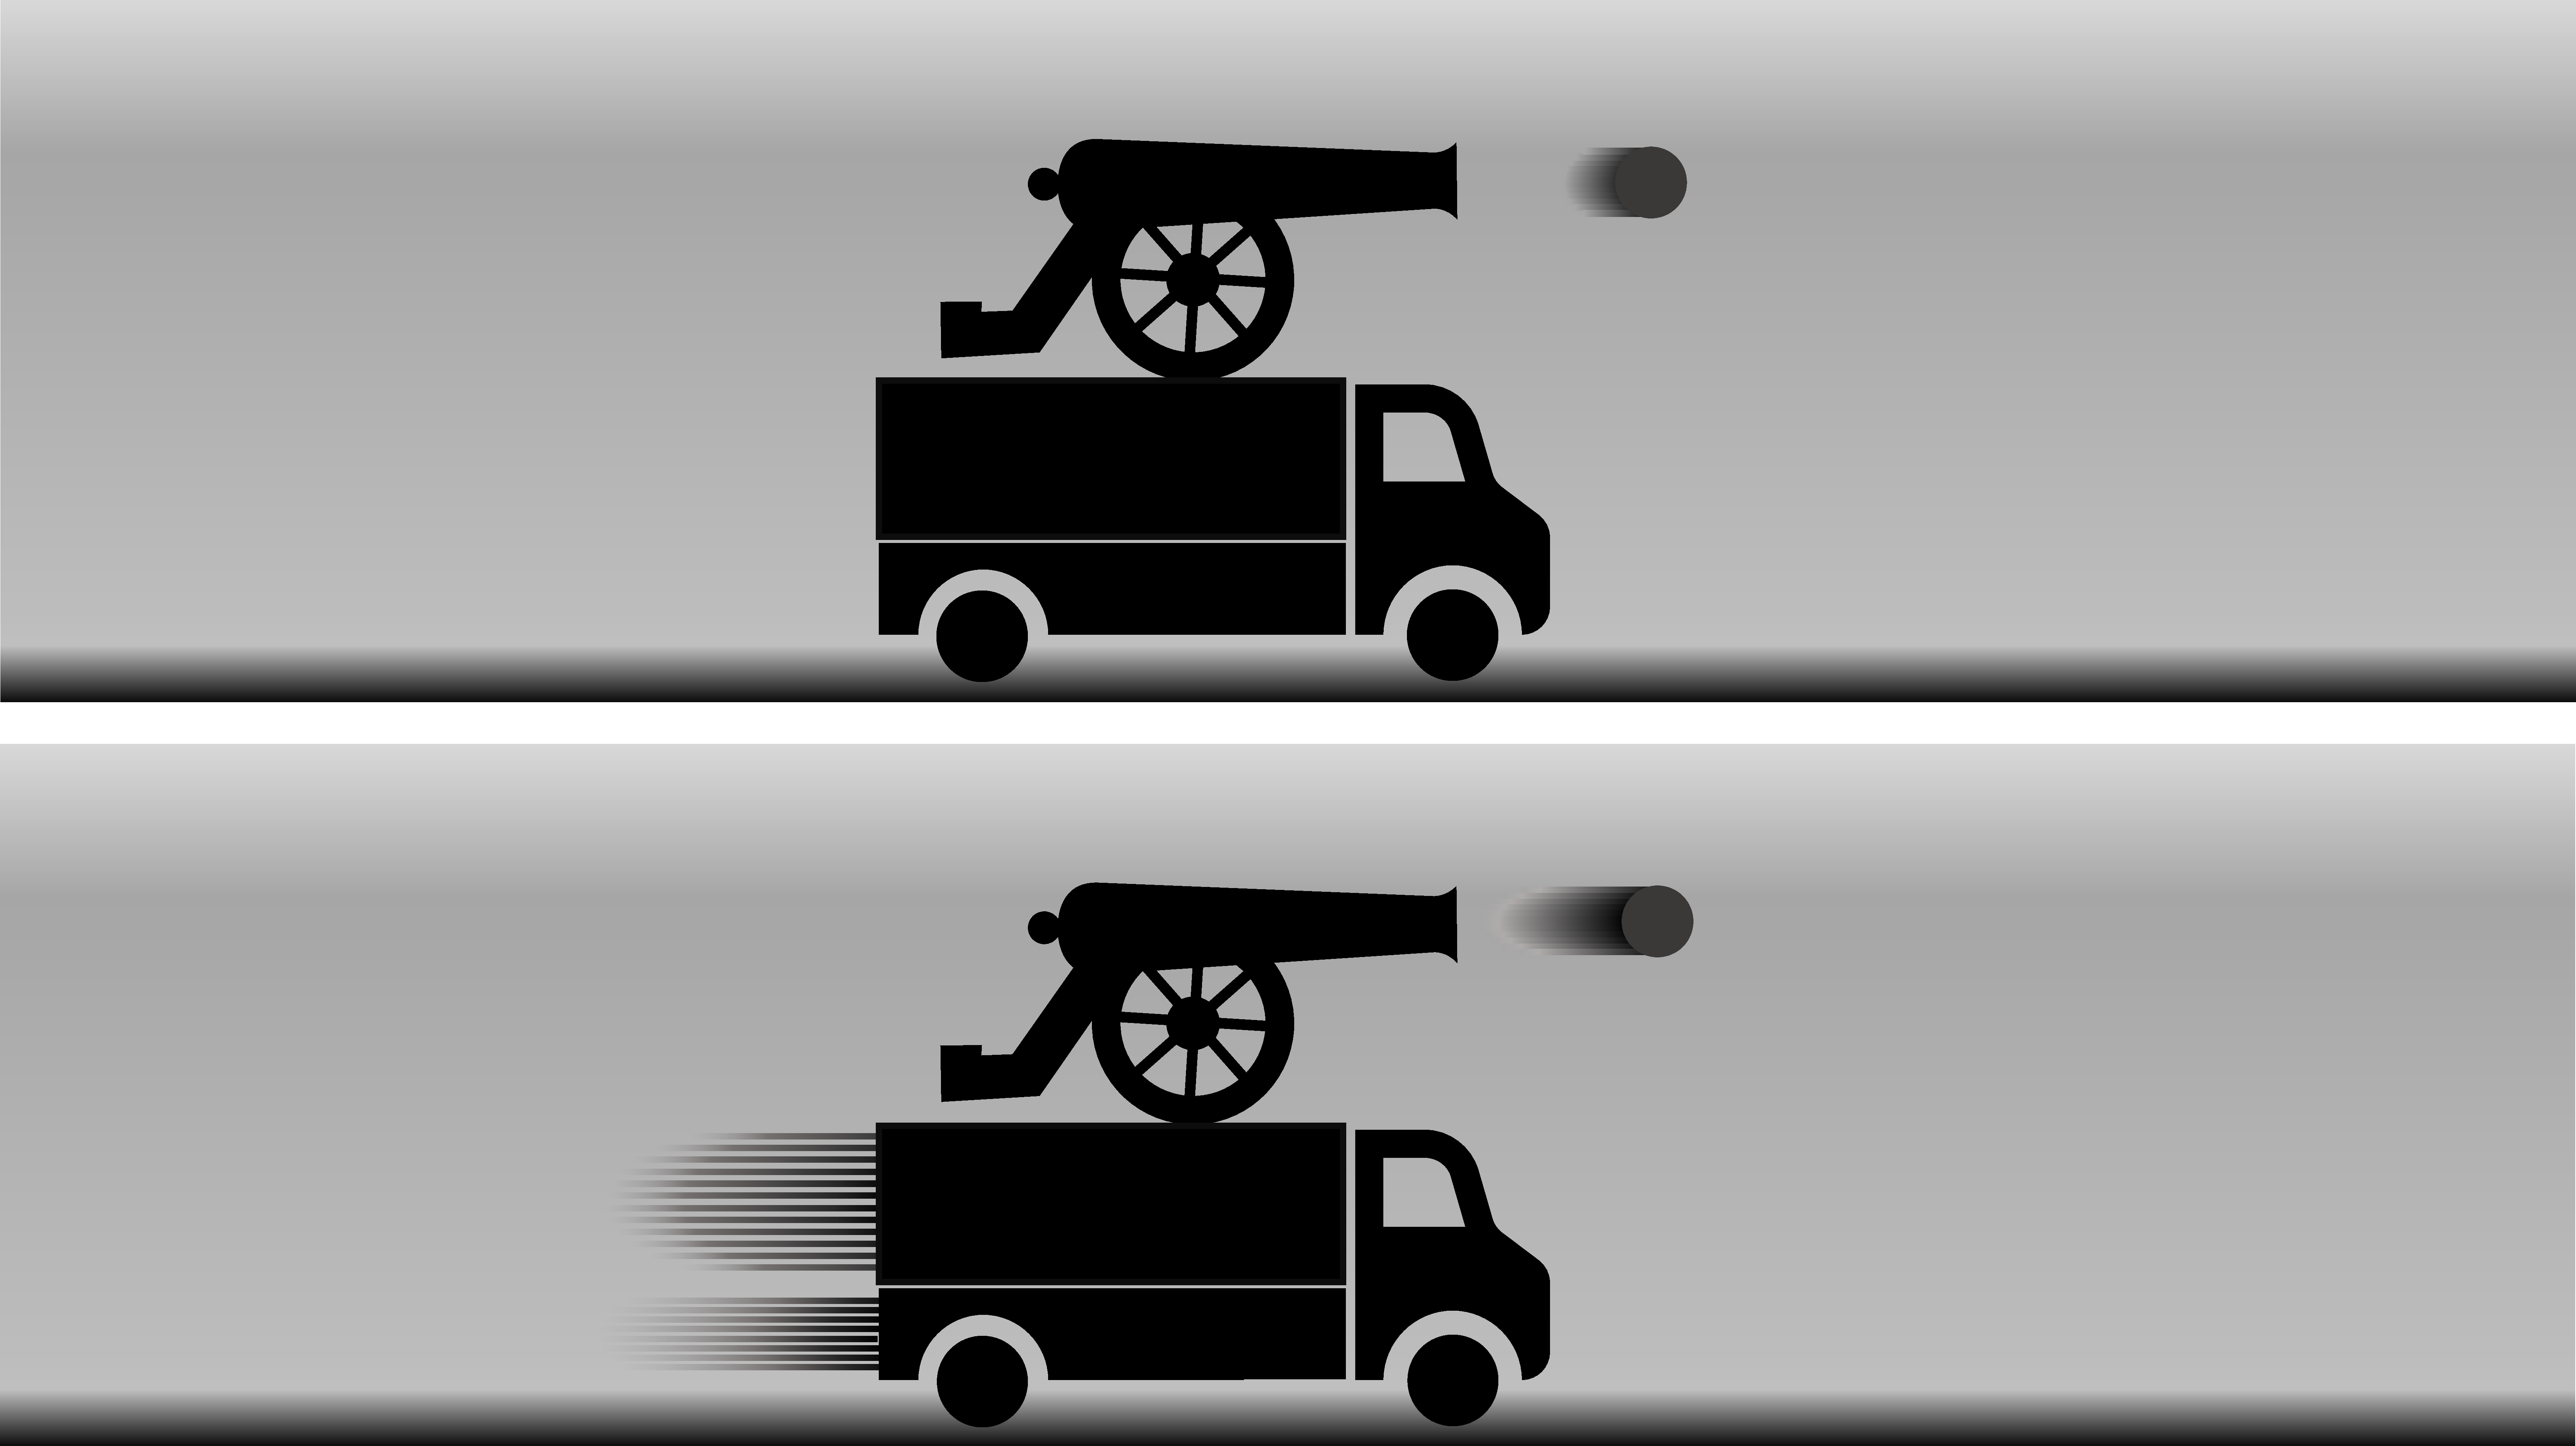
\includegraphics[width=8cm]{lorry_cannonball.pdf}
    \caption{Diagram, showing the speed of cannon ball from two different perspectives, (top) is from someone's perspective who is on the truck who sees the cannon at rest with the road moving backwards, the cannonball is shot and is moving forward. (bottom) is from someone's perspective who is at rest on the road and sees the truck and cannon moving relative to them, when the cannonball is shot it looks like it is moving forward faster for them, as it seems to have the cannonballs velocity plus that of the truck it was shot from.}
    \label{fig: truck cannonball}
\end{figure}

Let us imagine that a truck is moving forward on a road at a constant speed of 20 m/s (meters per second), on the top of that truck, is a cannon that fires a cannonball in the same direction the truck is moving. The ball travels at a speed of 300 m/s relative to the truck. Classically to find out how fast the ball is moving relative to the road, we add the speed of the truck and the speed of the ball together: 20 + 300 = 320 m/s. So we find the ball is moving at a speed of 320 m/s relative to the road, and this is what we observe. So in classical physics, velocities directly add, the ball relative to the road would move at the speed of the ball relative to the truck plus the truck 's speed relative to the road. 
But this turns out to just be a very good approximation for objects in our normal day life which we are used to seeing, which are moving much slower than the speed of light (which is roughly 300 000 000 m/s), but we will get to this later. For now we will explain more about the classical view, so that you will be able to see more clearly the differences when it comes to special relativity.

%███████████████████████████████████████████████████████████████████
%███████████████████████████████████████████████████████████████████
\section{Inertial Reference Frame}



\begin{figure}[H]
    \centering
    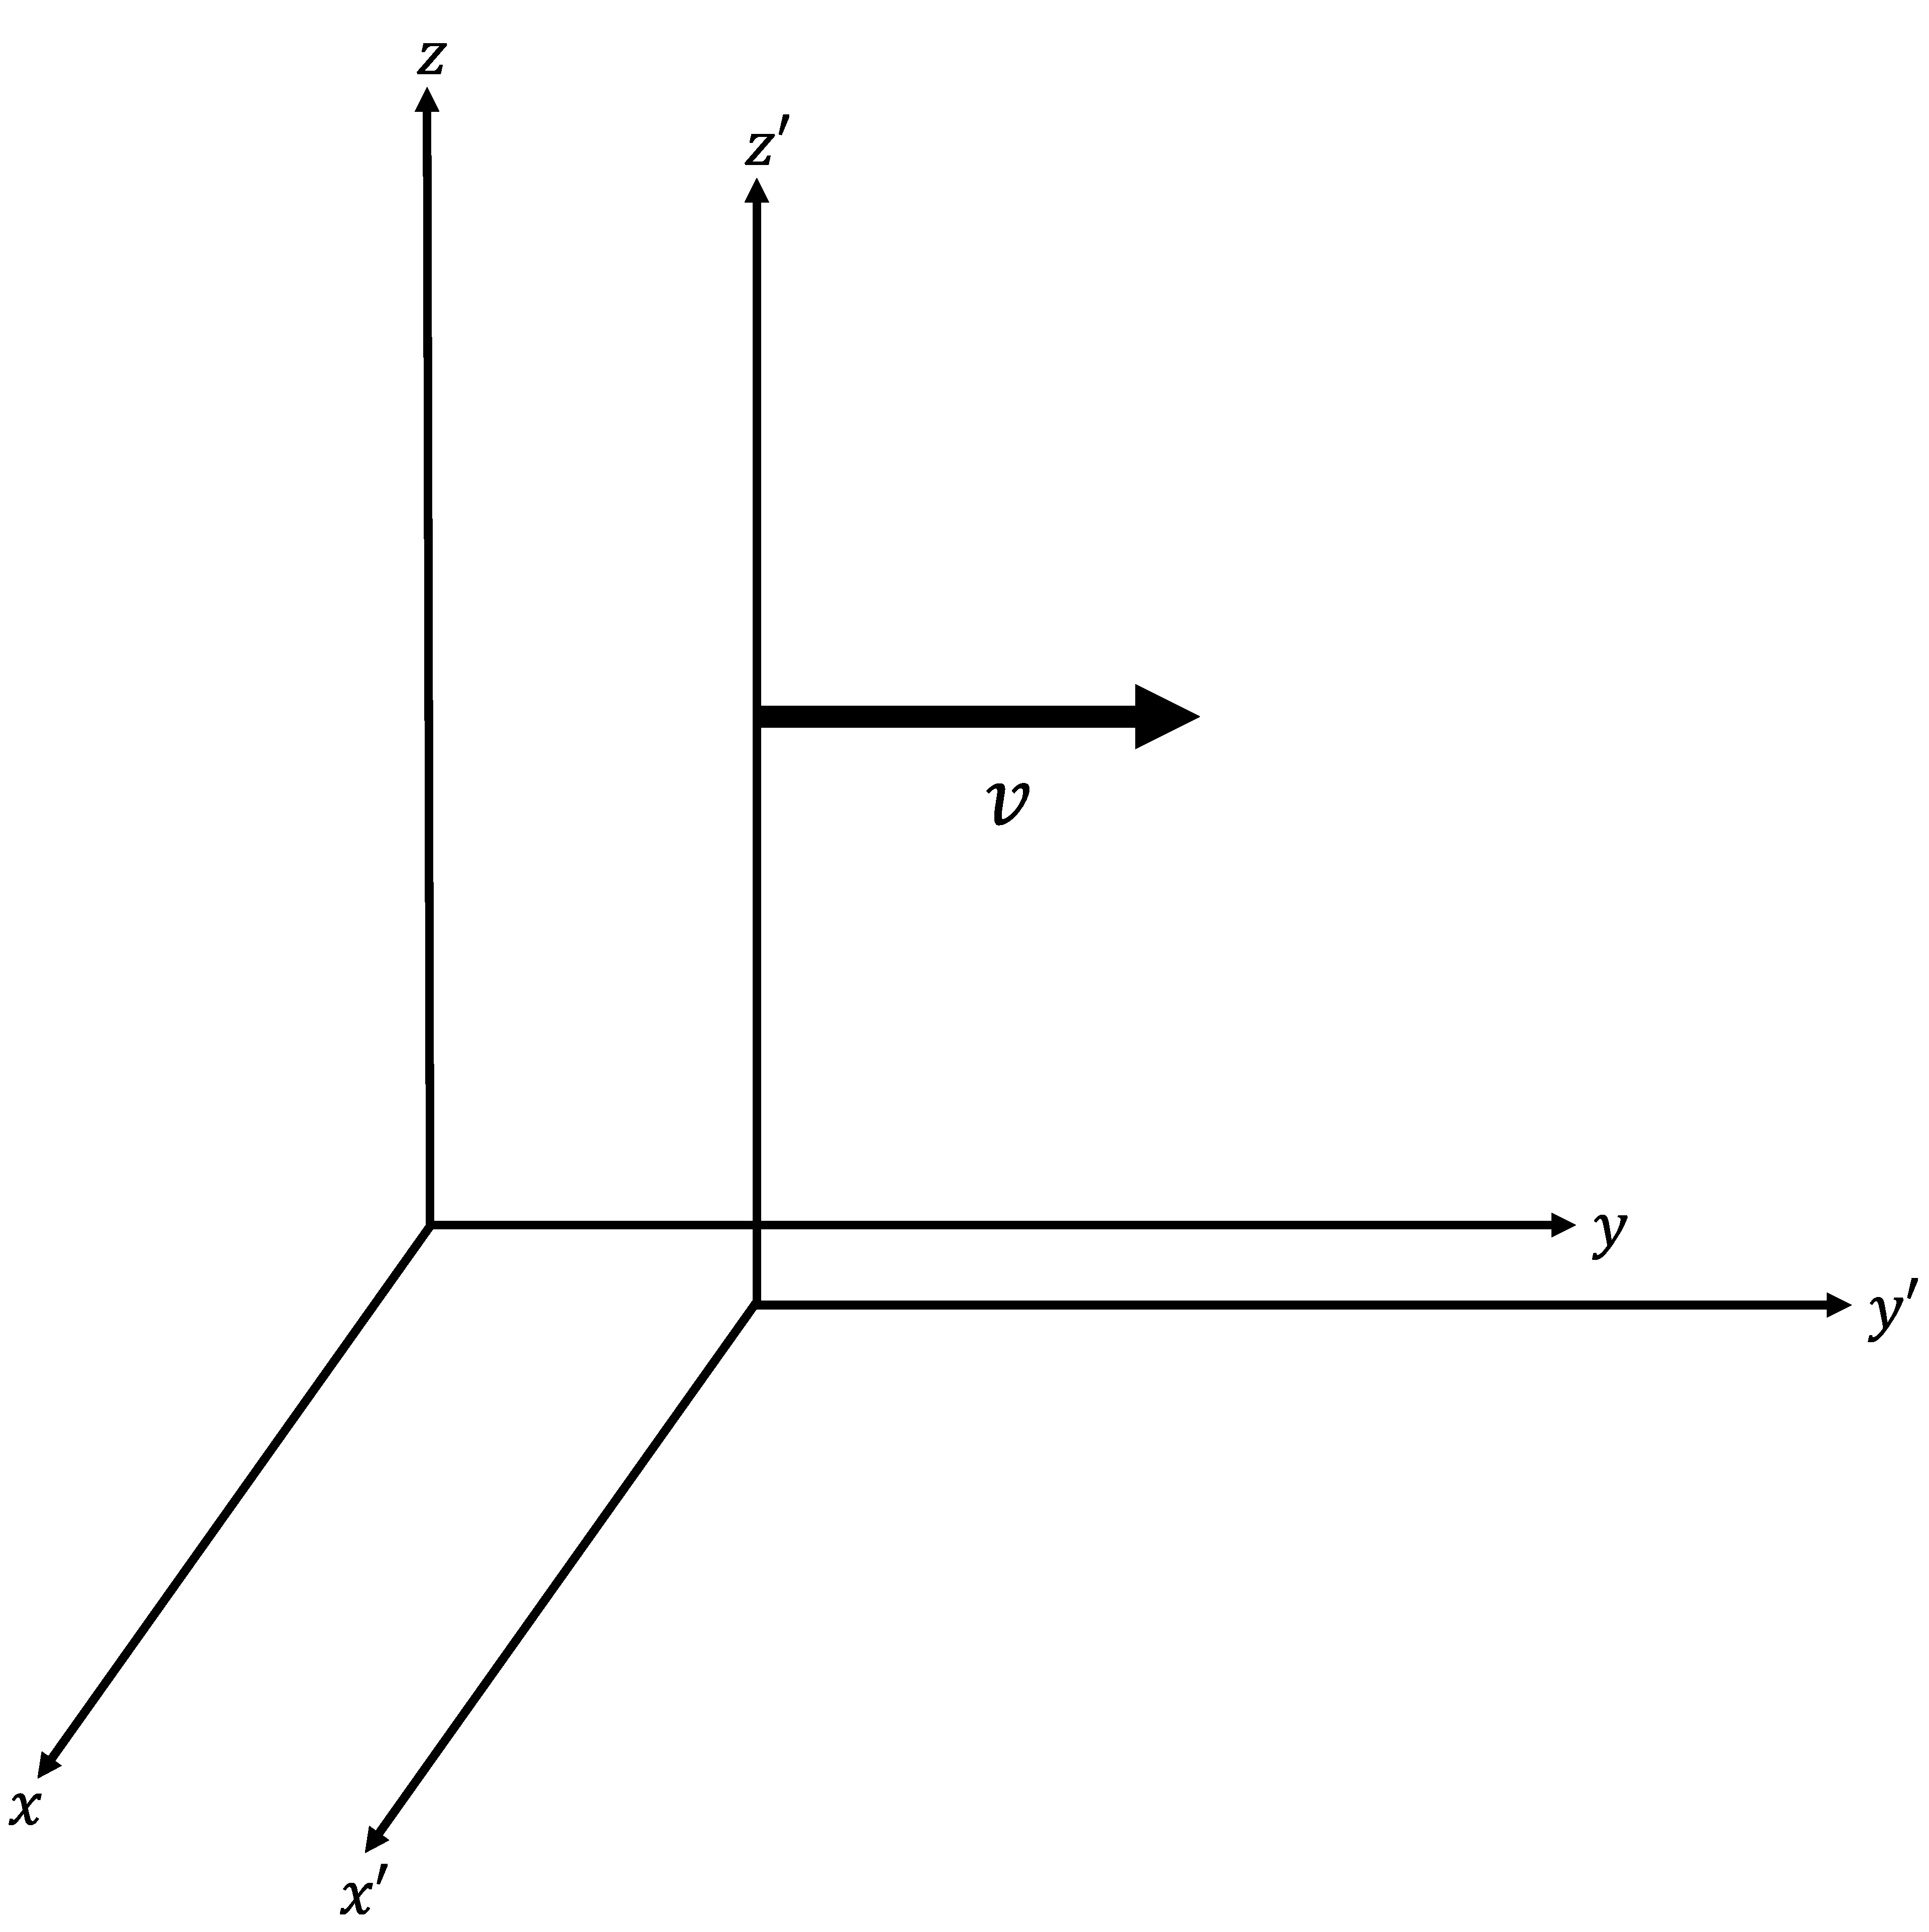
\includegraphics[width=0.35 \textwidth]{Reference Frames.pdf}
    \caption{Diagram of a \protect\hyperlink{def-Reference-frame}{reference frame} moving relative to another.}
    \label{fig:Reference Frames}
\end{figure}


A \hyperlink{def-Reference-frame}{reference frame} can be thought of as an abstract coordinate system. The origin of its axis, its orientation, and its scale are specified by a set of points in space. The purpose of it is to provide a standardised means of measuring and describing the coordinates of objects within that frame at any instant of time.

An \hyperlink{def-Inertial-reference-frame}{inertial reference frame}, is one that is not undergoing any acceleration. You can tell if you are being accelerated, as you will feel a force, take for example, in an accelerating car you will feel the chair being accelerated into you, with your body slightly lagging behind in the acceleration, and its this basic principle for how accelerometers measure acceleration as shown in the diagram. 
%((a note on free fall being inertial frame))

\begin{figure}[H]
\centering
       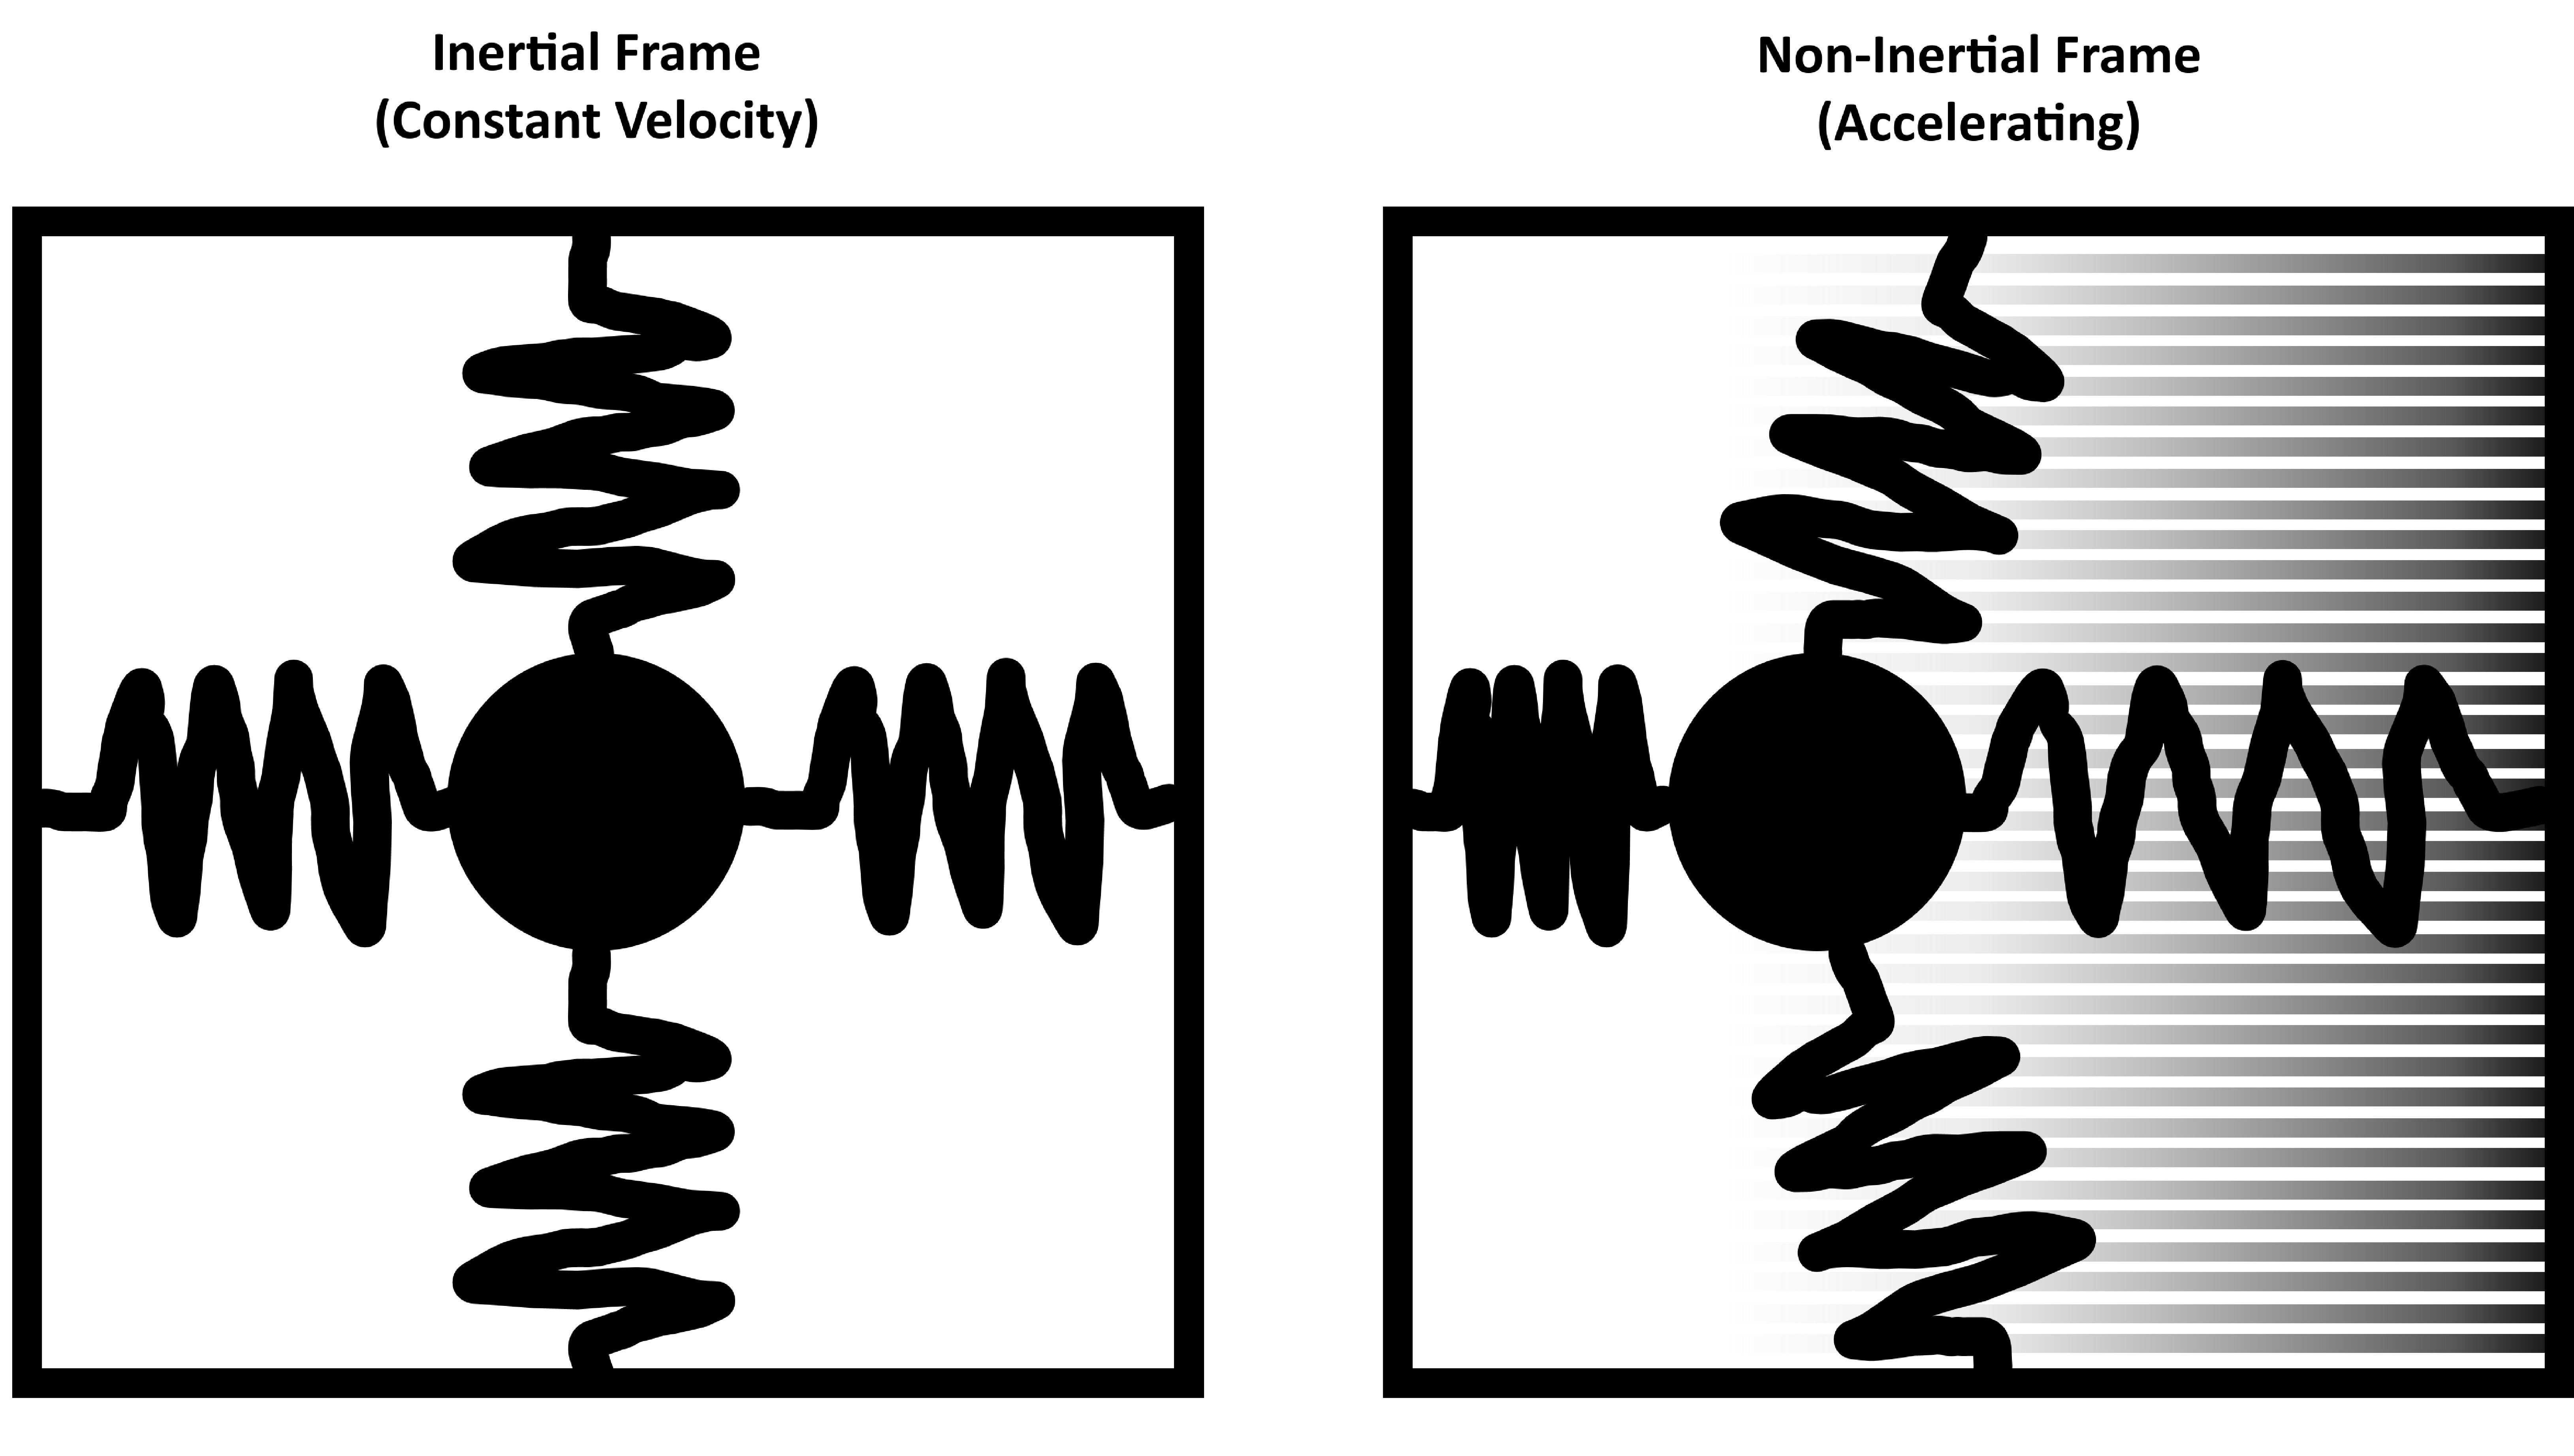
\includegraphics[width=\textwidth]{Spring_boxes.pdf}
    \caption{Diagram of a ball, attached to the walls of a box by springs, with the ball centred in the box in the inertial frame, i.e. with no acceleration (left), and in an non-inertial frame (right) where the box is now accelerating to the right, The ball lags behind as the box accelerates.}
    \label{fig: spring boxes}
\end{figure}


%███████████████████████████████████████████████████████████████████
%███████████████████████████████████████████████████████████████████
\section{Classical Reference Frames}

To see how to swap between \hyperlink{def-Reference-frame}{reference frame}s in special relativity we will first have to introduce what the classical swapping between two \hyperlink{def-Reference-frame}{reference frame}s look like. To help us understand this, we will use a system of a moving platform, like we find on a treadmill. The two frames of reference will be that of the treadmill's platform and the room in which it is in.

\begin{figure}[H]
    \centering
    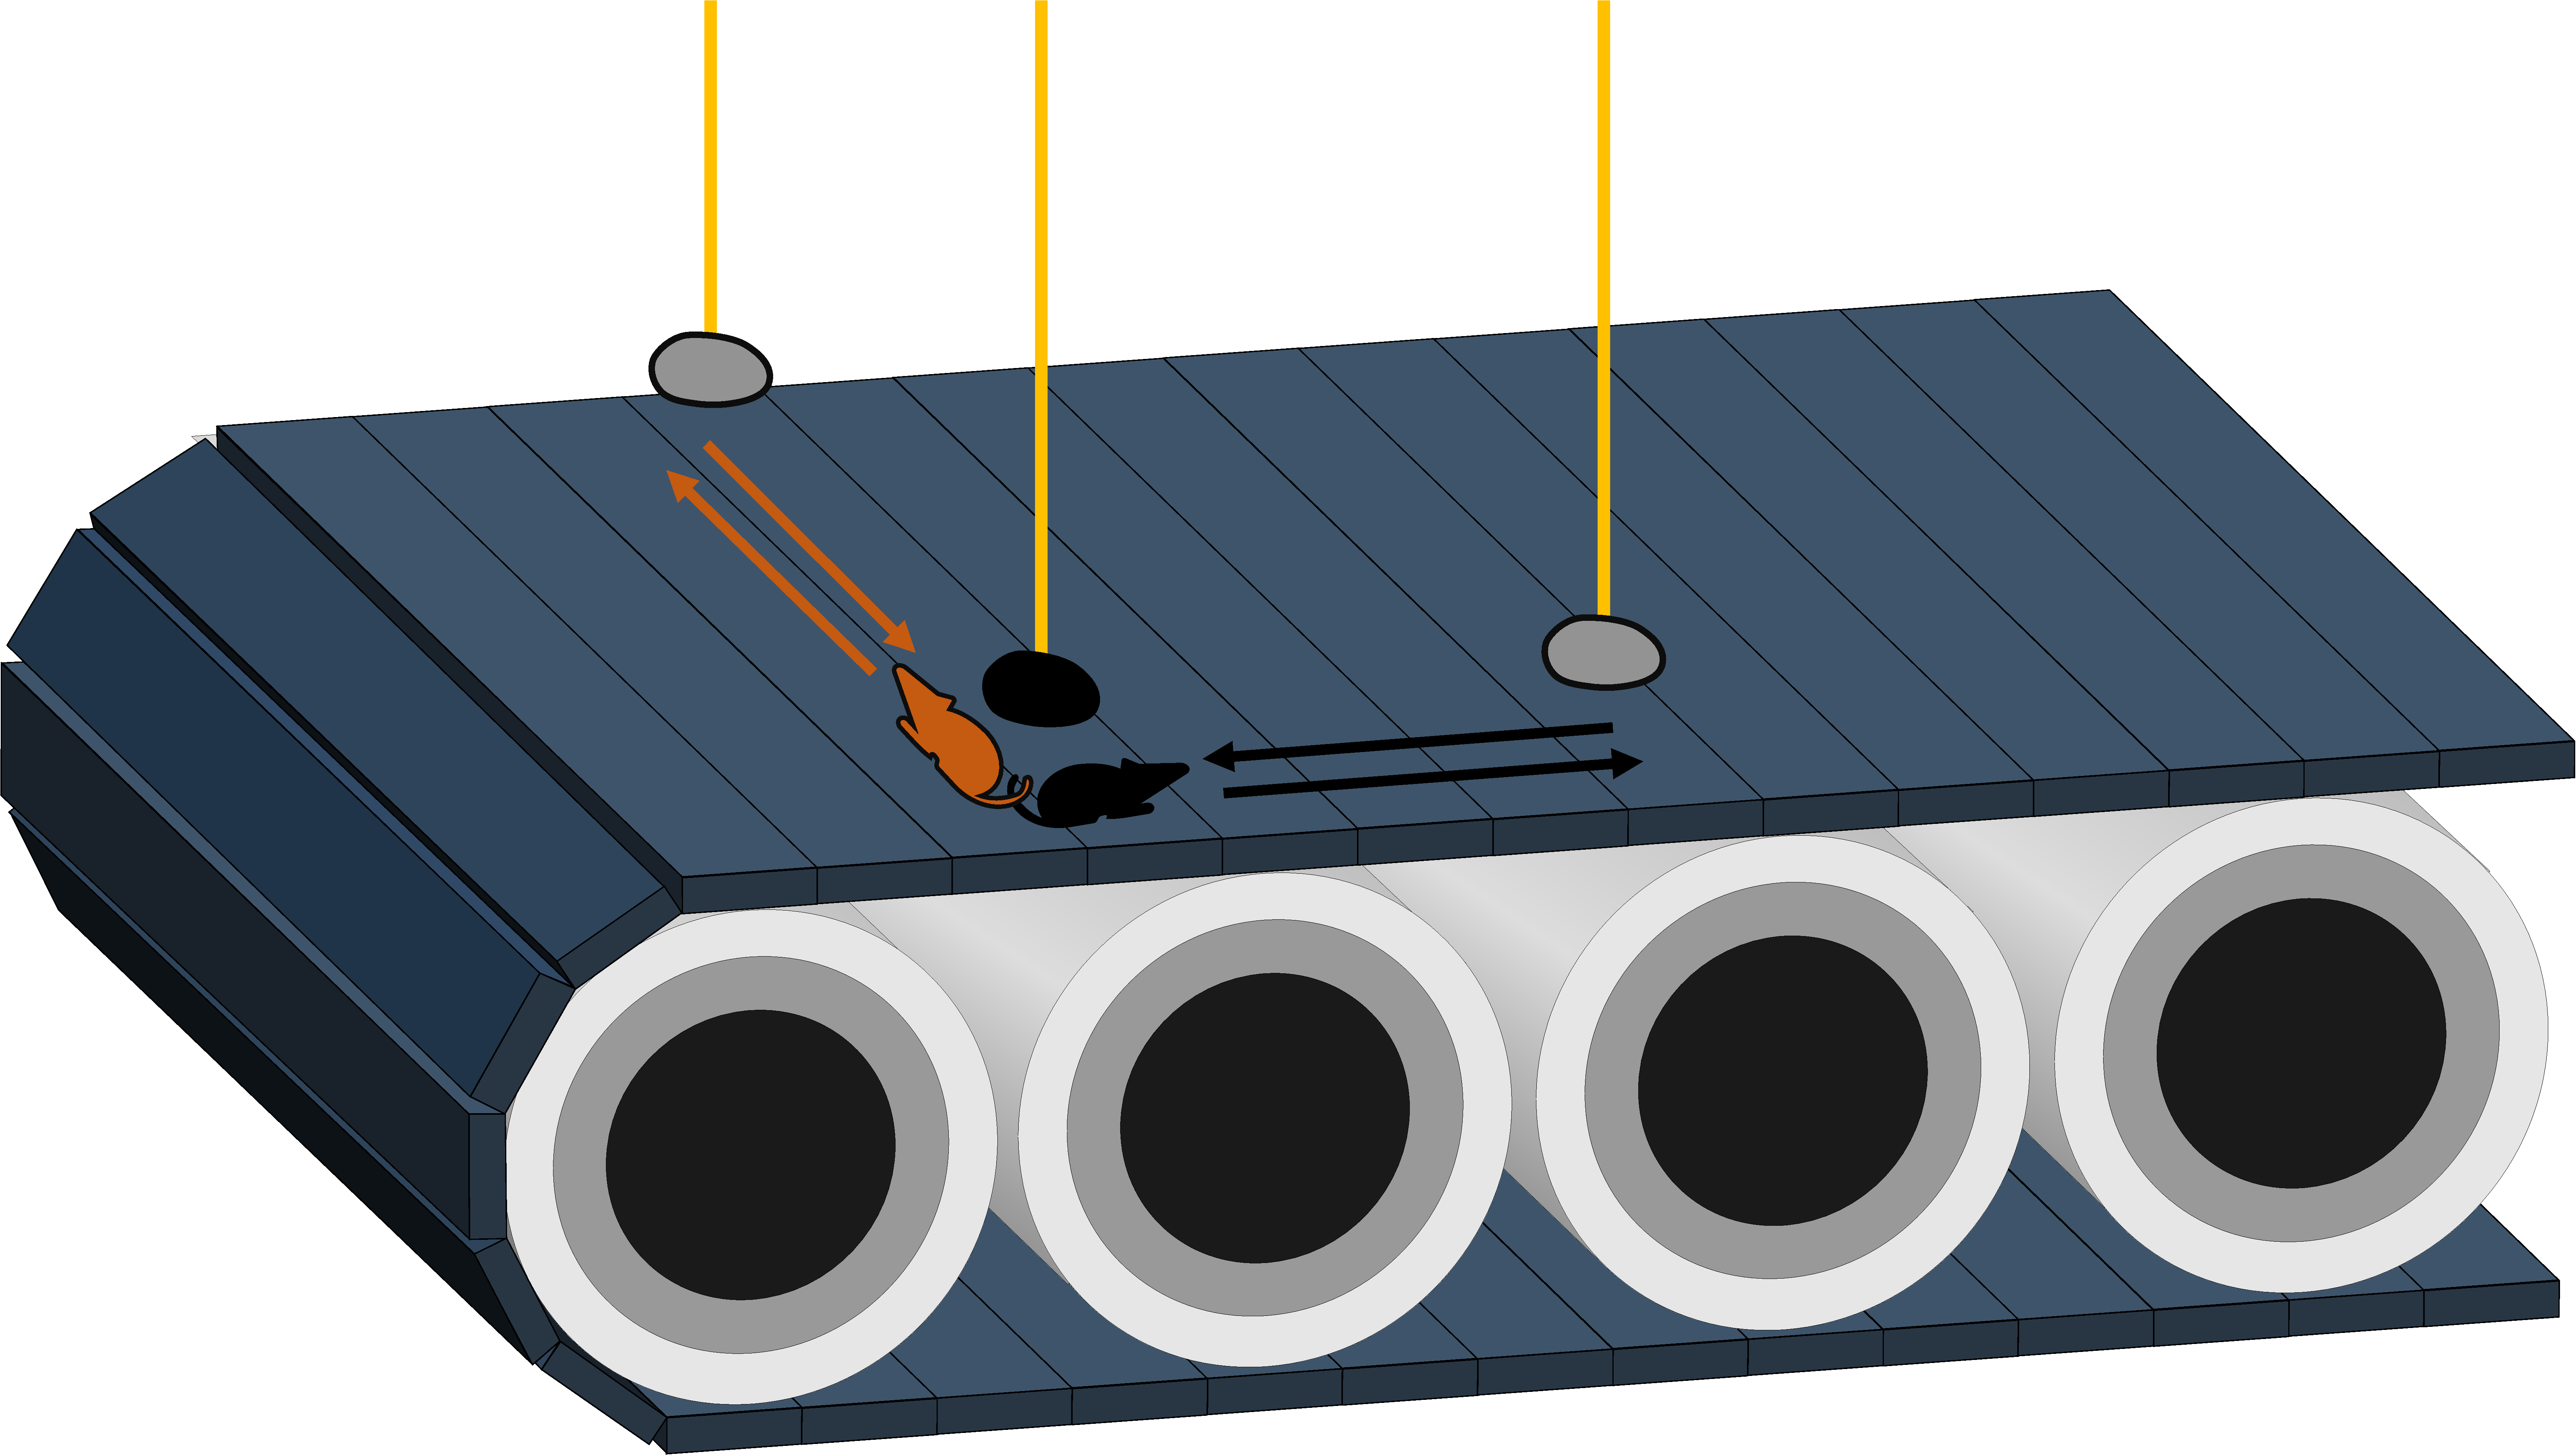
\includegraphics[width=\textwidth]{Conveyor_belt_3d.pdf}
    \caption{Diagram of 3d view of treadmill platform, with two rats and three hanging rocks.}
    \label{fig: 3d conveyor belt}
\end{figure}

To illustrate swapping between frames classically, We will look at a setup of two rats on a treadmill as shown in Figure \ref{fig: 3d conveyor belt}, with three rocks hanging above the platform, at rest relative to the room. Both rats start under the same rock, one runs to a rock positioned in the forward direction of the treadmill, and the other runs to an equally distanced rock to the side, they then return to the starting rock. Here the platform can be seen as the medium in which the rats move. Both rats travel at the same constant speed relative to the platform, with the platform at a lower speed than the rats to allow them to get to the rocks. 

If the platform is at rest, they will return to the starting rock at the same time. But if the treadmill is turned on and the platform is now moving, the rats will now have to also work against the movement of the platform to get to the rocks, this will lead to different distances the rats have to travel, and as a result the rats get back to the starting rock at different times. The figures \ref{fig: rat with moving platform} and \ref{fig: rat platform reference frame} show what the direction of movement of the rats and rocks look like in each \hyperlink{def-Reference-frame}{reference frame}.

\begin{paracol}{2}
\begin{figure}[H]
\centering
    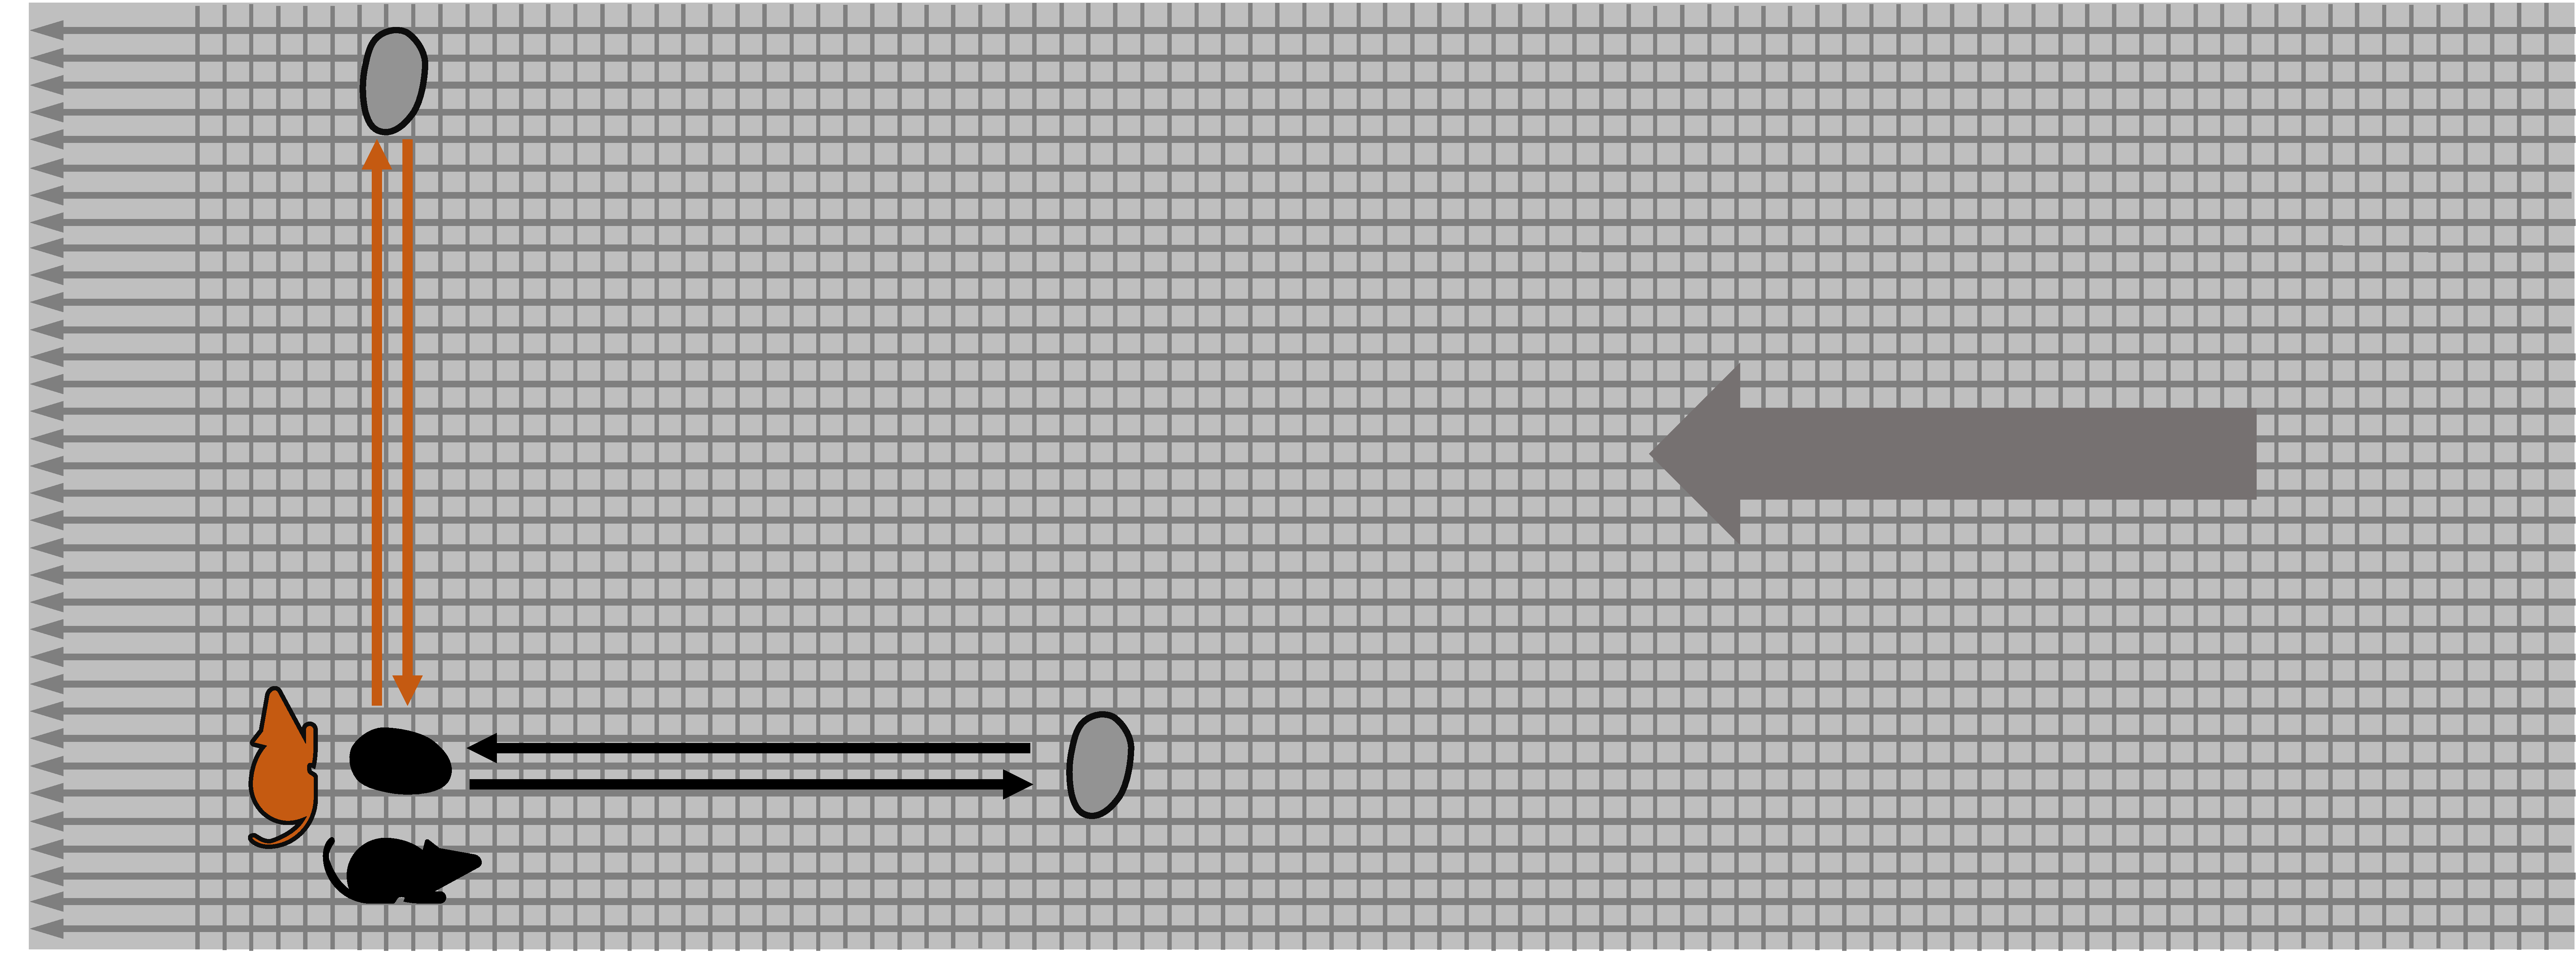
\includegraphics[width=0.45\textwidth]{rats_moving.pdf}
    \caption{Rats on moving platform, from room's \protect\hyperlink{def-Reference-frame}{reference frame}.}
    \label{fig: rat with moving platform}
\end{figure}
\switchcolumn
\begin{figure}[H]
\centering
       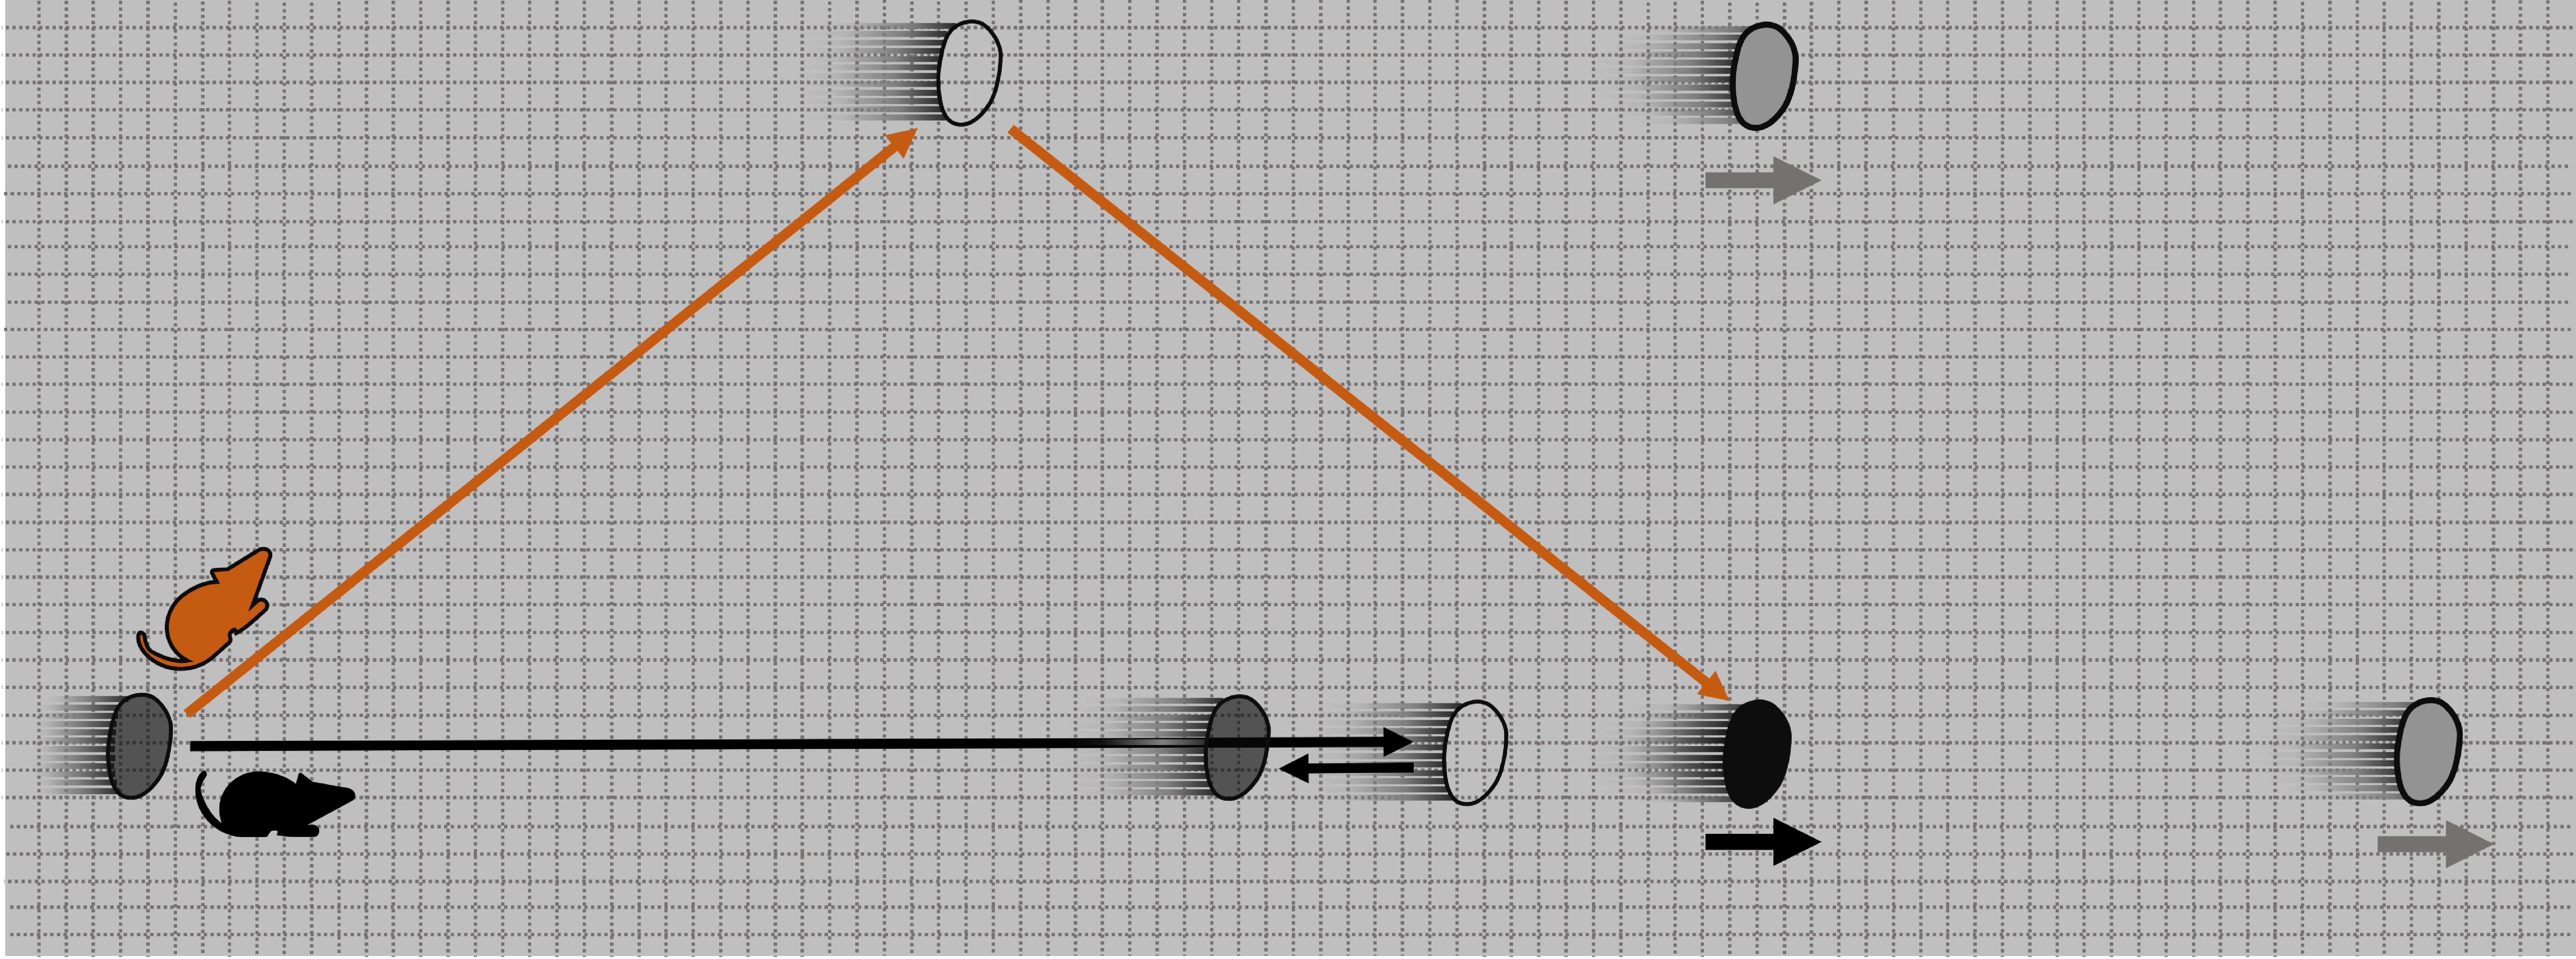
\includegraphics[width=0.45\textwidth]{rats_platform_frame.pdf}
    \caption{Rats on moving platform, from platform's \protect\hyperlink{def-Reference-frame}{reference frame}.}
    \label{fig: rat platform reference frame}
\end{figure}
\end{paracol}

\iffalse javascript{Rats_treadmill} \fi

In the room's \hyperlink{def-Reference-frame}{reference frame} we have the platform moving backwards, the rat moving straight ahead will have impedance to its movement but after it turns around it now has a boost from the platform to get back to the starting rock, were as the sideways moving rat will have to go sideways and also balances out the backwards pull of the platform to keep a perpendicular movement towards the hanging rocks. This gives different lengths of paths depending on the \hyperlink{def-Reference-frame}{reference frame}, as shown in figures \ref{fig: rat with moving platform} and \ref{fig: rat platform reference frame}. It also gives different times for the rats to return to the starting rock. This is what we would expect and see with this classical example of frame swapping, but next we will look at whether we can have the same sort of frame swapping when it comes to light travelling in two different frames of reference, and the notion of a universal \hyperlink{def-proper-frame}{rest frame} referred to as the \hyperlink{def-aether}{aether}.

%███████████████████████████████████████████████████████████████████
%███████████████████████████████████████████████████████████████████
\section{The Aether}%, a Medium for Light} % and a Universal Rest Frame}


\begin{figure}[ht]
\centering
       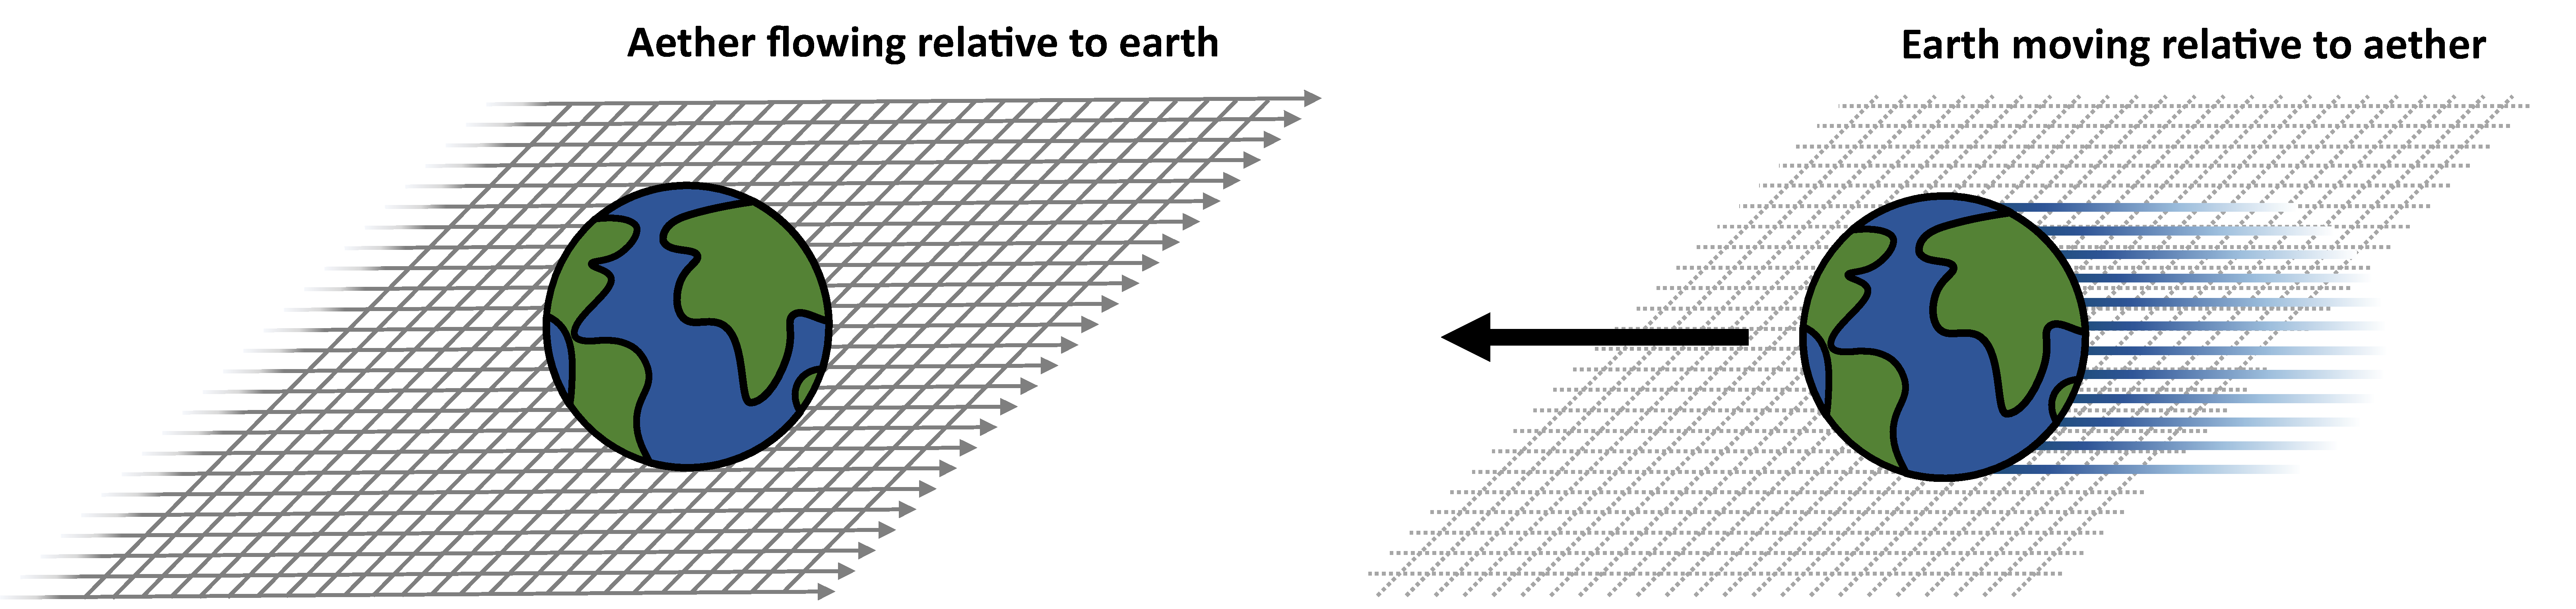
\includegraphics[width=\textwidth]{earth_and_aether.pdf}
    \caption{A diagram showing the \protect\hyperlink{def-aether}{aether}'s and earth's movement relative to each other.}
    \label{fig: Aether}
\end{figure}

In the 1800's, the theory was that light was a wave and therefore would need a medium for it to travel through that filled the \hyperlink{def-vacuum}{vacuum} of space, called "the luminiferous \hyperlink{def-aether}{aether}", and that light would travel at a constant speed relative to this \hyperlink{def-aether}{aether}, like how the rats in the previous section moved at a constant speed relative to the medium of the treadmill's platform.

An experimental setup by Michelson and Morley, shown in Fig. \ref{fig: Michelson_morley}, was devised to measure earth's movement through the \hyperlink{def-aether}{aether} \cite{EtherExperiment}, by measuring how it affected the speed of light in different directions, when observed in earth's \hyperlink{def-Reference-frame}{reference frame}. 

\begin{figure}[H]
\centering
       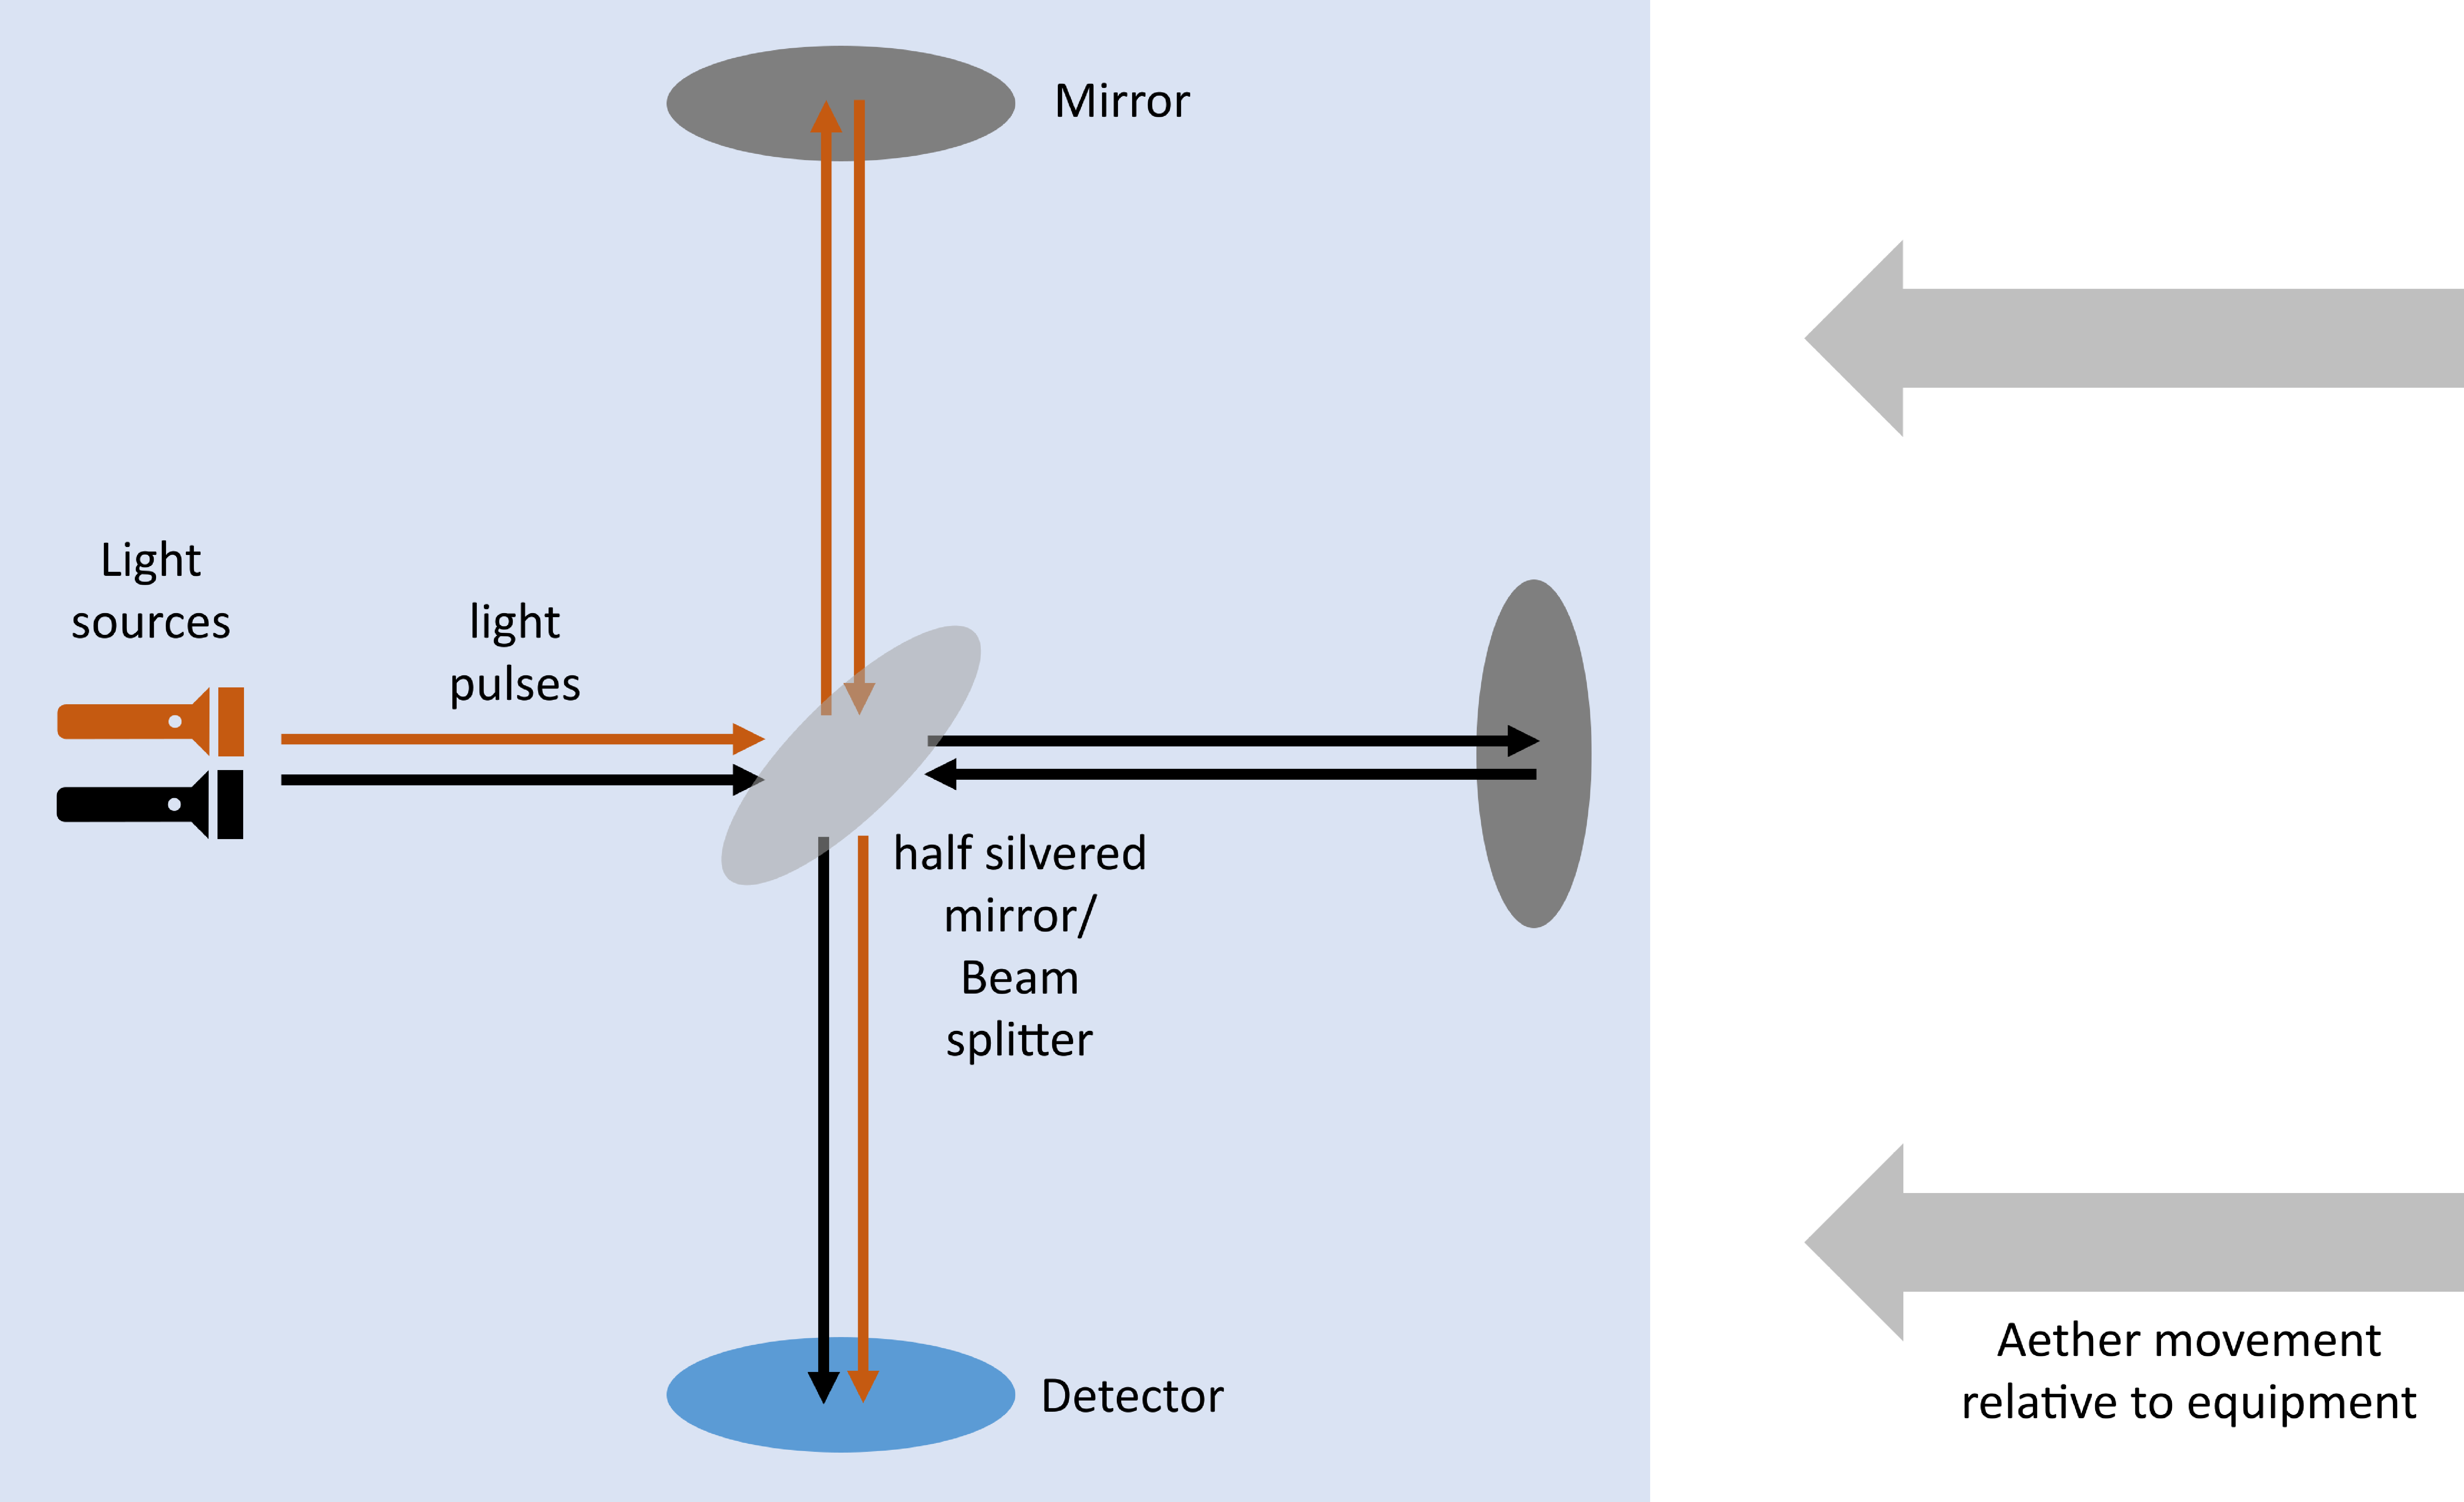
\includegraphics[width=8cm]{Michelson_morley.pdf}
    \caption{A diagram showing the Michelson-Morley experiment, (we can take the part of the paths between the the beam splitter and two mirrors to be analogous to the case of the paths in the previous rat and treadmill diagrams) }
    \label{fig: Michelson_morley}
\end{figure}

It did this by splitting a single light beam into two perpendicular paths, that are then reflected back to be recombined and sent towards a light detector. By rotating the whole interferometer setup, the two light paths could be aligned either parallel or perpendicular to the Earth’s motion through the presumed \hyperlink{def-aether}{aether}. 
They reasoned that if the speed of light was constant with respect to the proposed \hyperlink{def-aether}{aether}, that just as in the rat experiment from the previous section, the split light beams would recombine at different times. From the previous section the room is analogous to the room the experiment was carried out on earth, the treadmill's platform is analogous to the \hyperlink{def-aether}{aether} and the rats analogous to the light.
However, when Michelson and Morley performed the experiment, they found no difference in travel time to the detector for both paths, indicating that there was no difference in the speed of light in any direction in earth's \hyperlink{def-Reference-frame}{reference frame}. hence no dependence of lights speed on the supposed \hyperlink{def-aether}{aether}. This null result seriously discredited the \hyperlink{def-aether}{aether} theories and ultimately led to the proposal by Einstein in 1905 that the speed of light (in a \hyperlink{def-vacuum}{vacuum}) is a universal constant and independent on motion of \hyperlink{def-observer}{observer} or source. And to allow for us to have this universal speed of light (in a \hyperlink{def-vacuum}{vacuum}), it will require us to change our ideas of how time and positions are perceived by different \hyperlink{def-observer}{observer}s. 



%███████████████████████████████████████████████████████████████████
%███████████████████████████████████████████████████████████████████
\section{Speed of Light}% as a Constant}

The experiments showed light does not have a medium that it travels at a constant velocity relative too, but instead travels at a constant velocity in a \hyperlink{def-vacuum}{vacuum} in all \hyperlink{def-Reference-frame}{reference frame}s, independent of how fast the source of that light is moving in the frame, e.g. a moving truck's head lights. Light only moves slower in objects such as glass due to being impeded by the interactions between it and the material it is travelling through.

Light itself moves extremely fast compared to any other everyday speeds we are used to (roughly 300 000 000 m/s, it can travel the diameter of the world in the blink of an eye). This is why we do not notice any delay in things we see around us in everyday life, though we should keep in mind that there is this delay, e.g. the light we see from the sun was emitted by it eight minutes ago for it to reach us now, and the further an object is located from us, the further back in time we are seeing it because of this delay.

\begin{figure}[ht]
\centering
       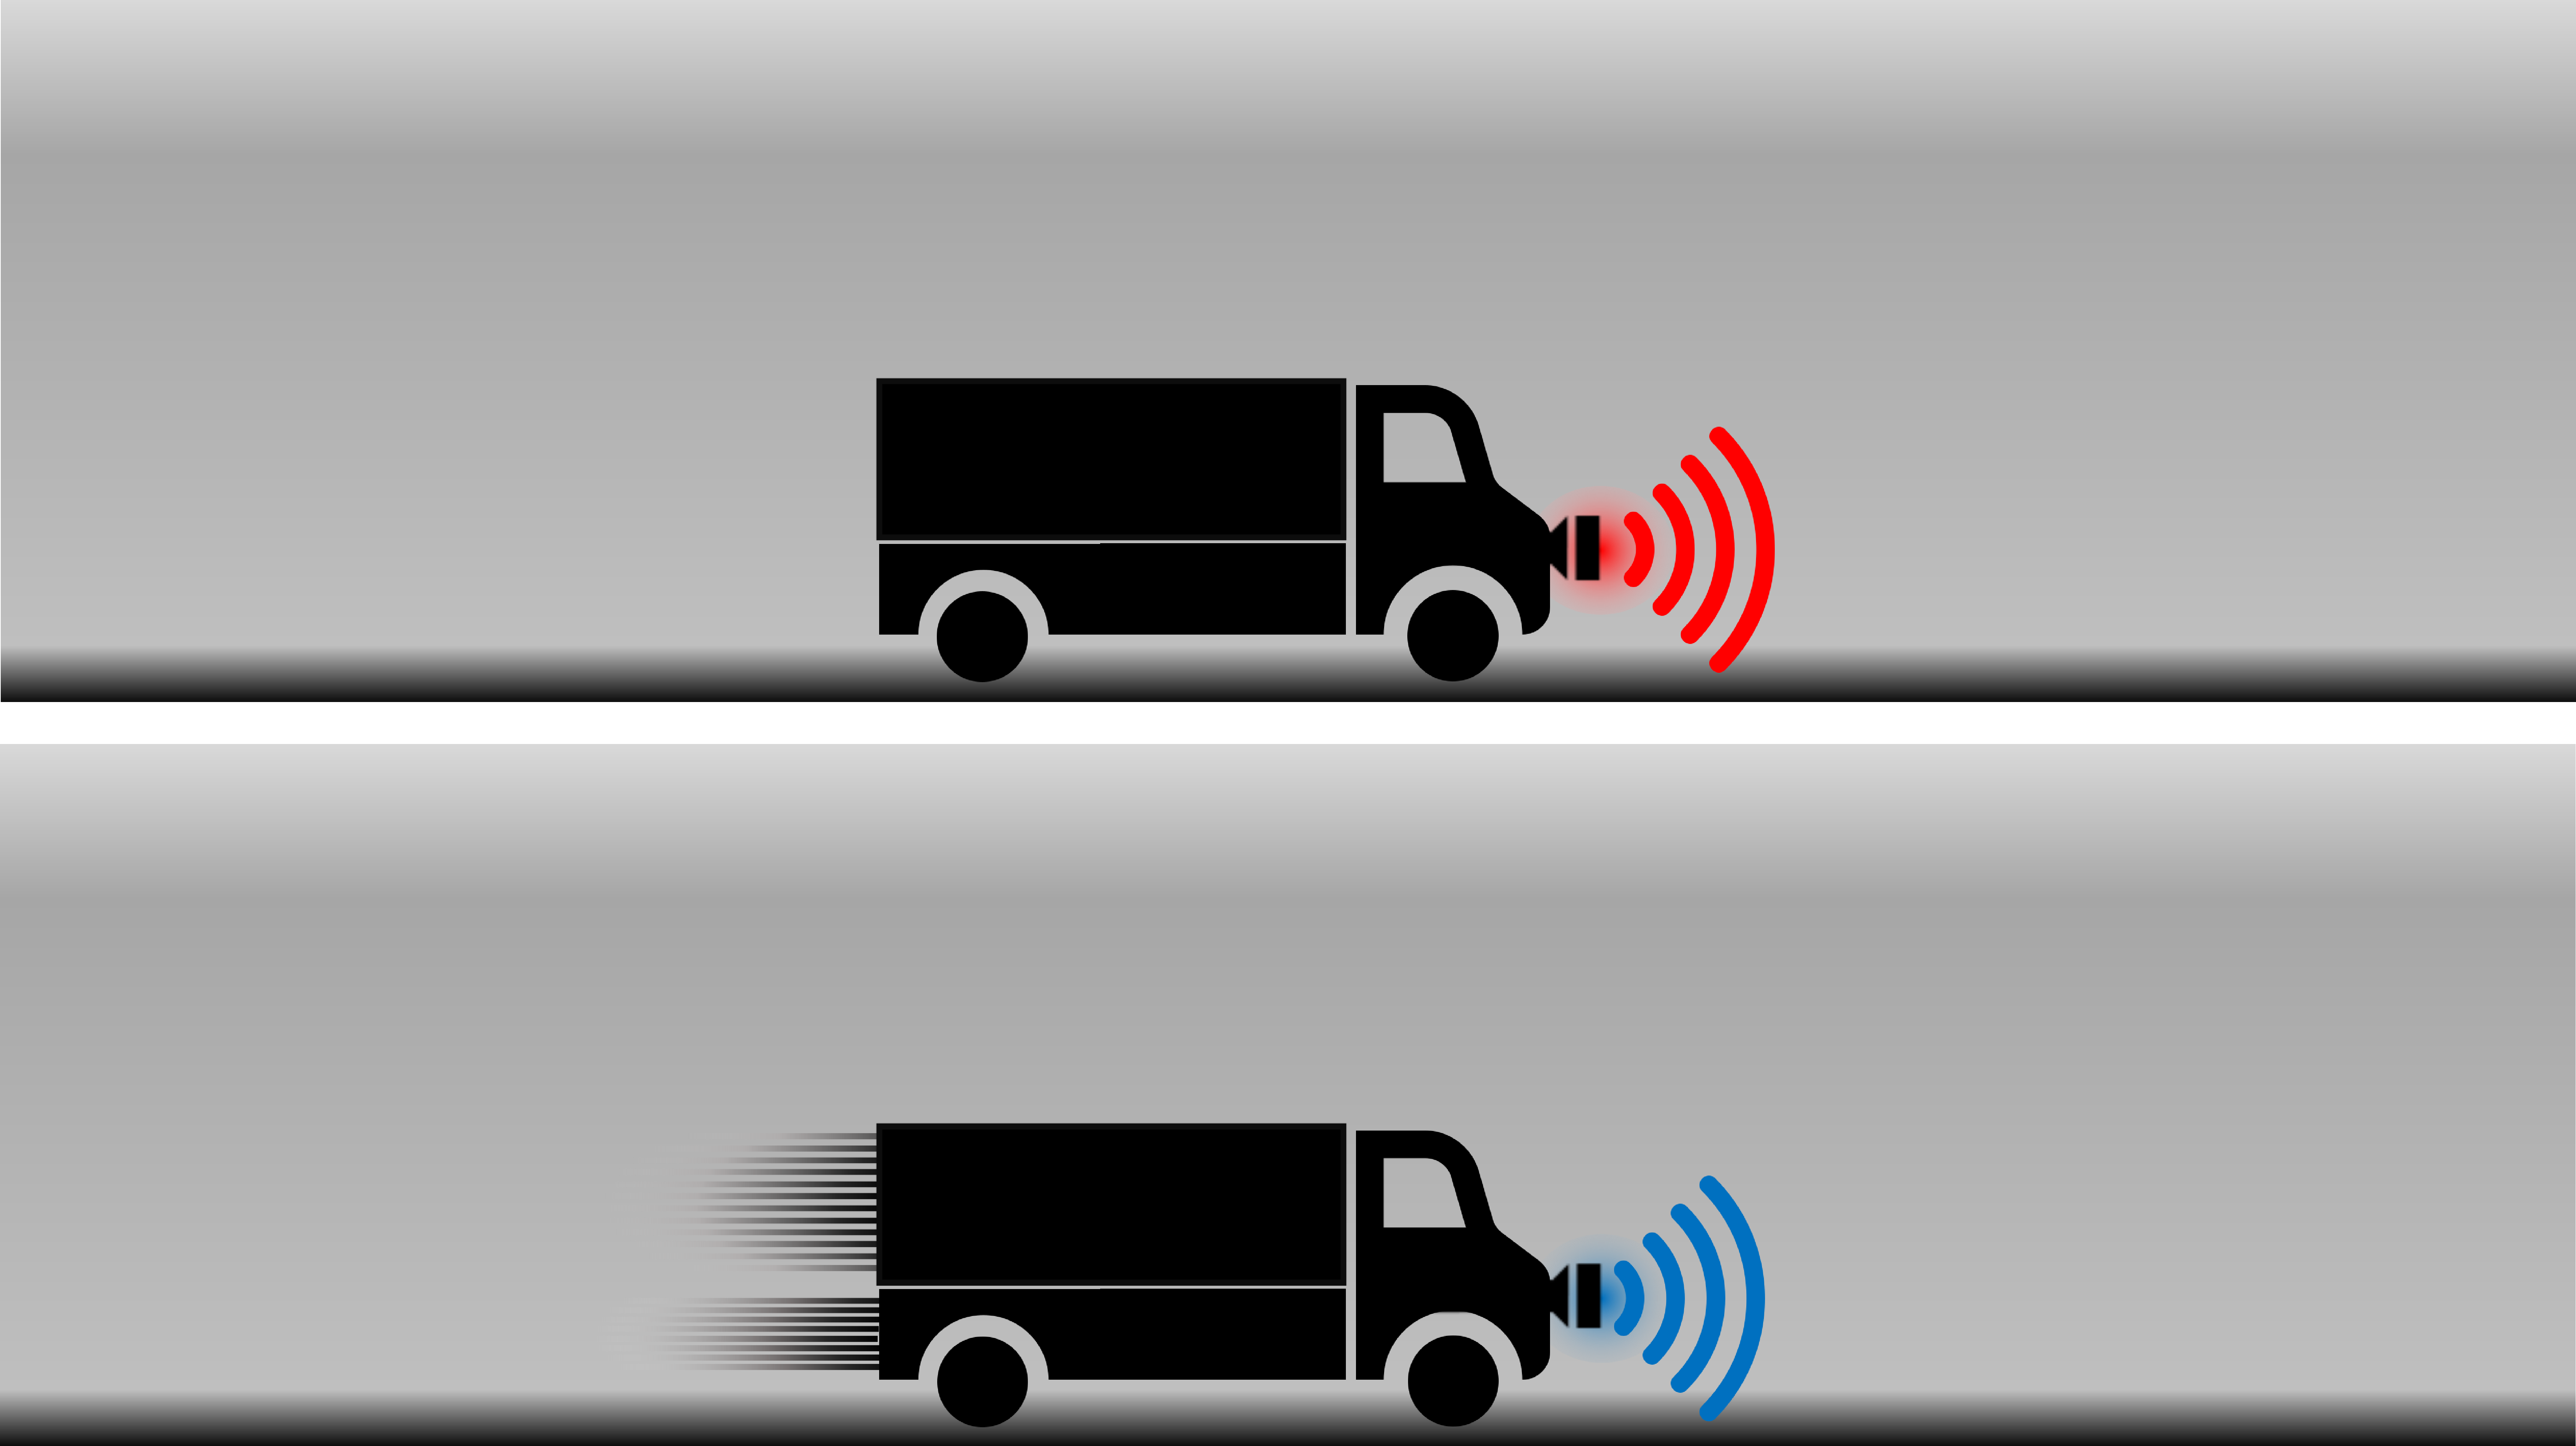
\includegraphics[width=8cm]{lorry_torch.pdf}
    \caption{A diagram, showing light emitted from a truck in two different \protect\hyperlink{def-Reference-frame}{reference frame}s, with the emitted light having the same speed in each frame, though with different frequencies/energies due to the \protect\hyperlink{def-doppler-effect}{Doppler effect}, which will be explained later.}
    \label{fig: truck torch}
\end{figure}


When we look at the same truck setup as the previous sections, but in a \hyperlink{def-vacuum}{vacuum} this time, where the cannon firing a cannonball is swapped for the headlights emitting light, it gives the same speed of light when measured relative to the truck or the road, but how can this be true?

For this to be true, we need a new way of thinking about velocity addition, since the velocities of objects have to be added in a way that is consistent with the requirement that the speed of light is constant, but also give approximate classical addition at speeds of objects at much less than the speed of light, like we observe with the cannon and truck. Since the speed of the light depends only on the units of time and positions, the only way to correct for this is to have the measured positions and times of objects \hyperlink{def-transform}{transform} differently when swapping between \hyperlink{def-Reference-frame}{reference frame}s than the classical way. This is what we will talk about next.
For the curious, it was the \href{https://scienceready.com.au/pages/determination-of-speed-of-light}{experiment by Ole Rømer} that showed that showed that light travelled at a finite speed rather than being instantaneously emitted and received. 


%███████████████████████████████████████████████████████████████████
%███████████████████████████████████████████████████████████████████
\section{Positions and Time}
%███████████████████████████████████████████████████████████████████
\subsection{Time Dilation}

\begin{figure}[H]
\centering
       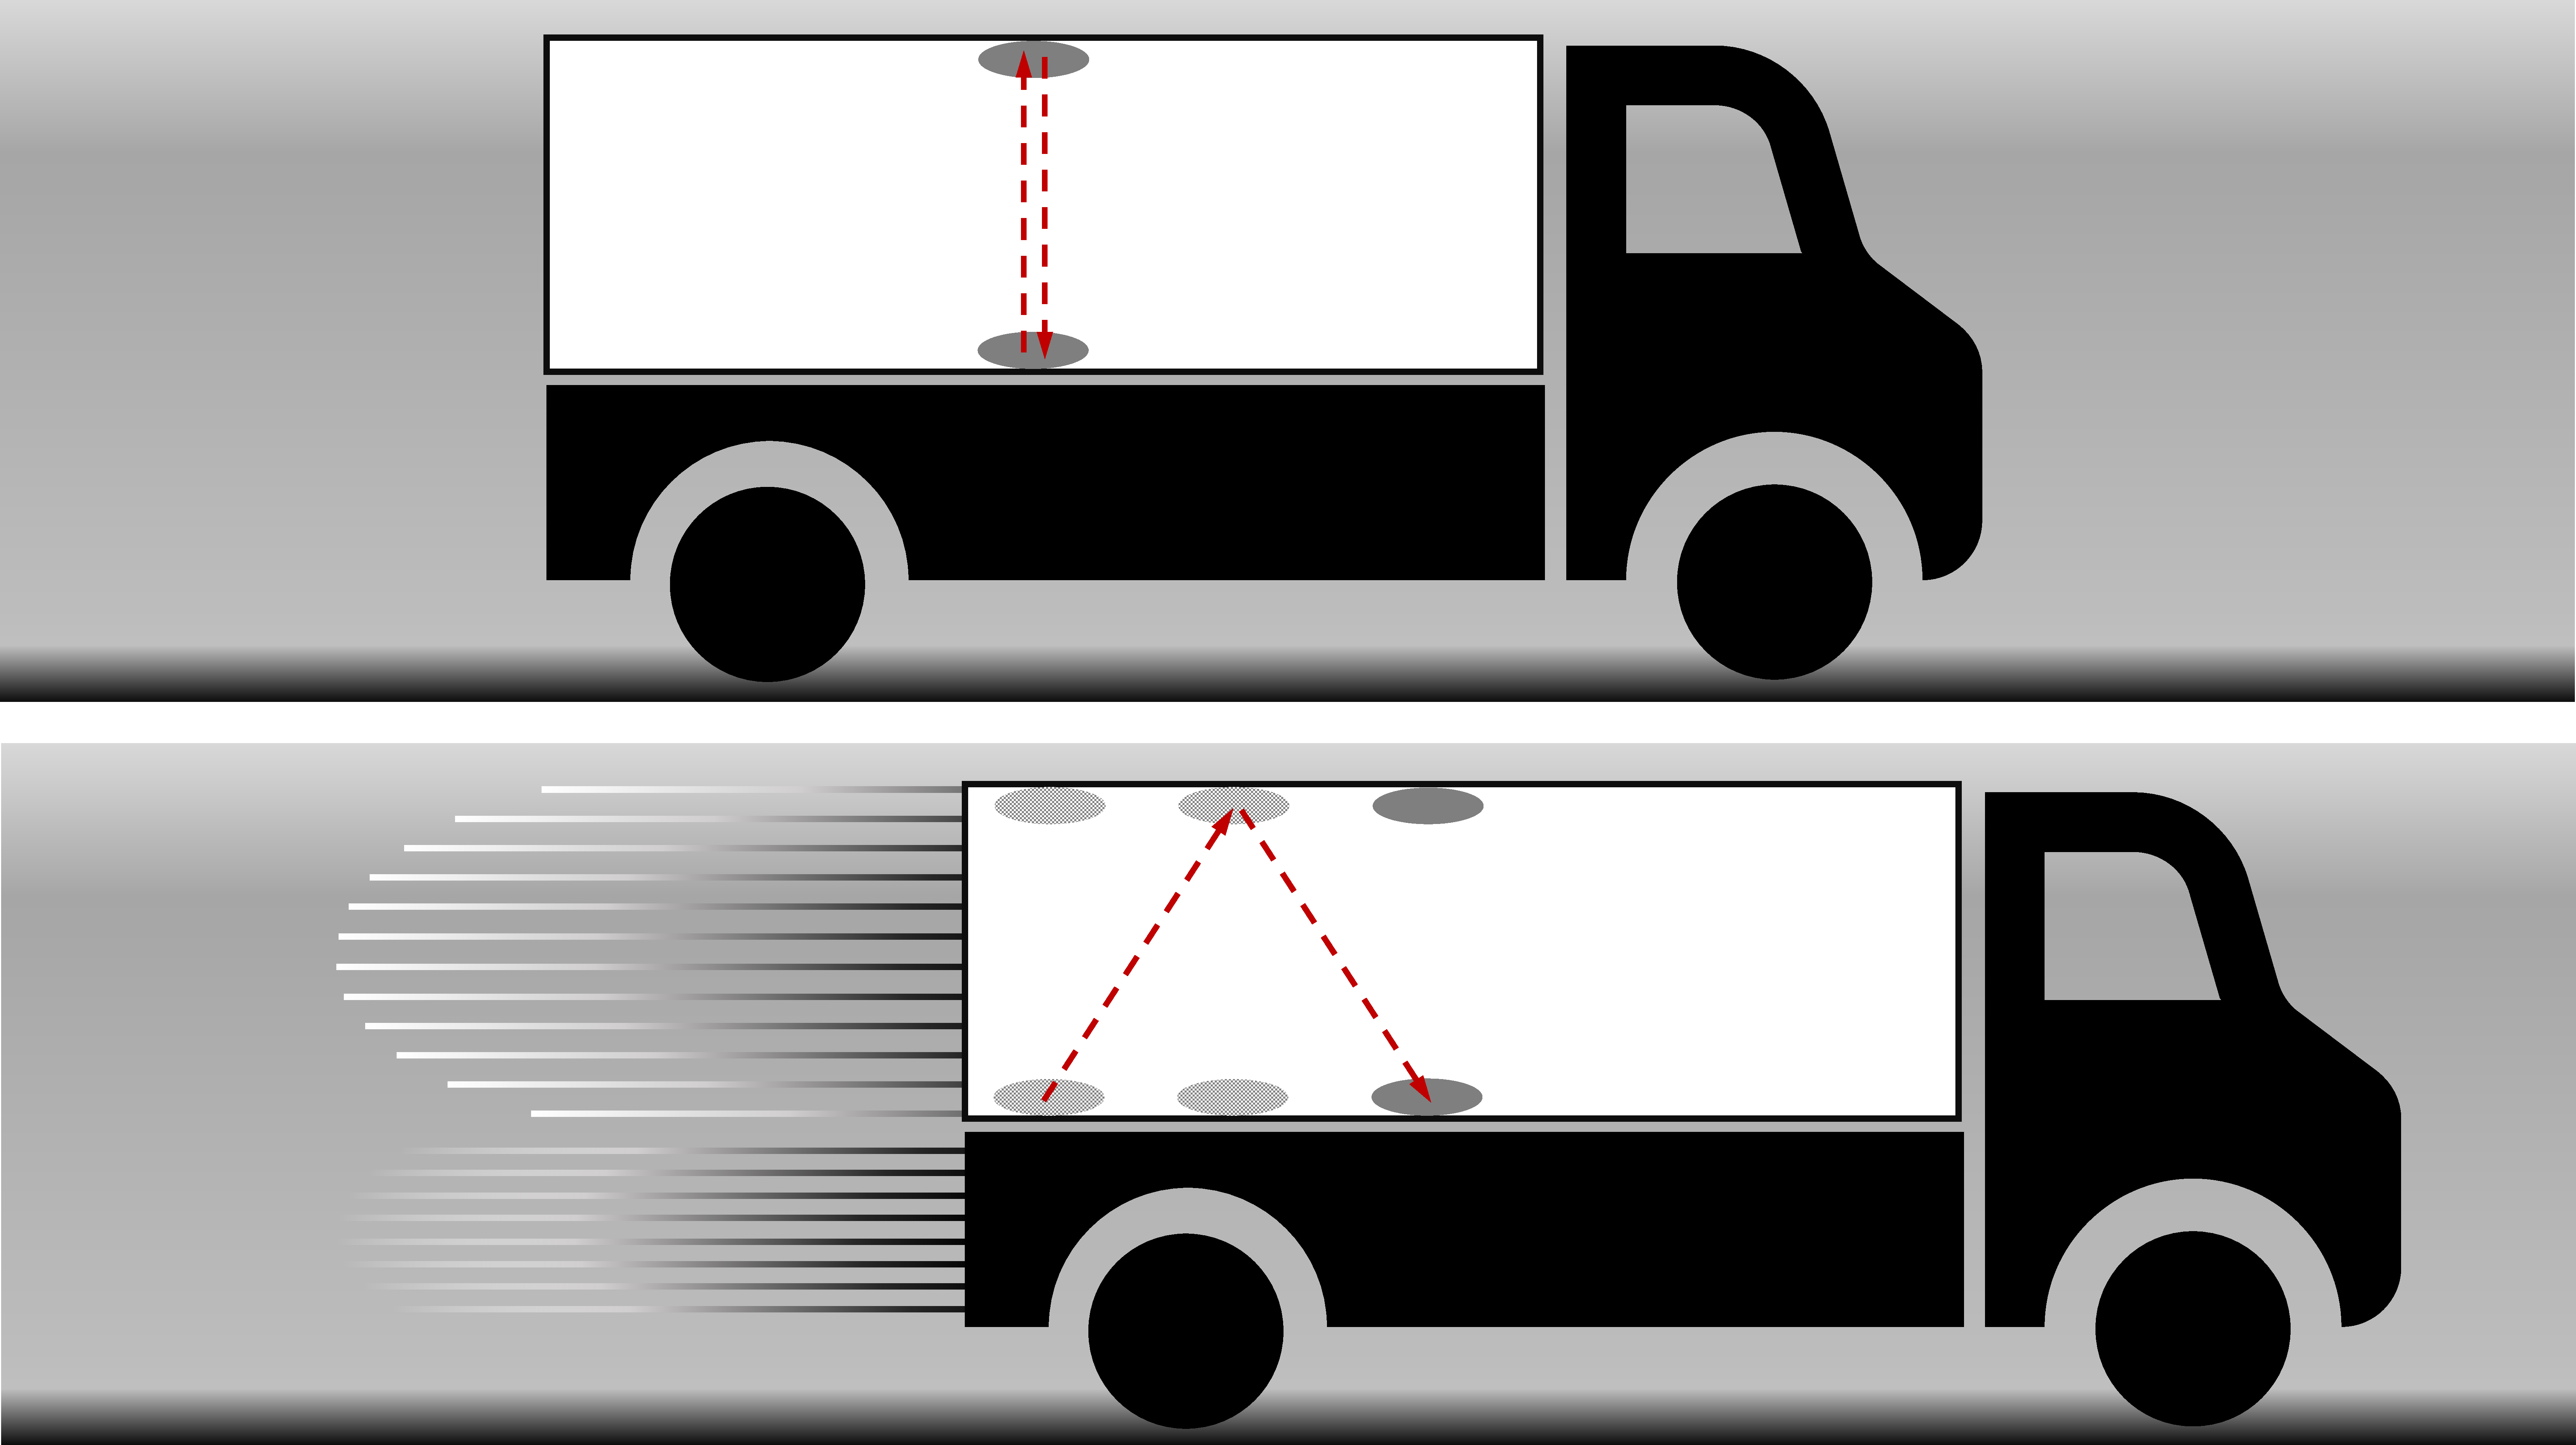
\includegraphics[width=8cm]{lorry_clock.pdf}
    \caption{Diagram showing the the extra distance light travels in the road's frame with truck moving}
    \label{fig: truck clock}
\end{figure}

Let us imagine a simple clock, as shown in Figure \ref{fig: truck clock}, made of a light pulse moving back and forth between two mirrors on a moving truck, with a mirror on the truck’s floor and on the roof directly above it, we will keep time by taking a tick of this clock to be when the light travels from one mirror to the other mirror and back again. For an \hyperlink{def-observer}{observer} in the truck, they will see the light go straight up and down between the mirrors, but an \hyperlink{def-observer}{observer} stationary relative to the road will see not just the light travelling up and down but also with the direction of the truck as well, hence it will travel a longer distance. But since the distance travelled by the light in the moving frame is longer and the speed of light is constant, we are only left with the possibility that the perceived travel time of the light has to be longer in this \hyperlink{def-Reference-frame}{reference frame}, i.e. the clock ticks slower to the \hyperlink{def-observer}{observer} on the road watching the moving truck. How much it is moving slower, can be solved using ratio of the lengths of paths in each frame as they are shown in the diagram. This difference in the flow of time will later lead to more odd consequences. The slowing of the ticking is also the same for any type of clock, and if you were to play a movie on the truck, it would take a longer amount of time for it to play through from the roads \hyperlink{def-Reference-frame}{reference frame}, it is the actual time itself being slowed down.

Also the closer the truck goes to the speed of light, the bigger the difference in how fast time flows relative to the truck 's time (this can be seen as a longer horizontal stretch in the path taken for the light from the perspective of someone standing still on the road).

% this section has so far assumed that the distances between the mirrors are not changed due to it being in a perpendicular directions to the motion of the truck , which will be addressed in a later section

%███████████████████████████████████████████████████████████████████
\subsection{Simultaneity}


%so events that happen simultaneously in different locations to an observer in the truck , happen at different times according to the road observer. this is the consequence of the need for speed of light to be constant to each observer.

\begin{figure}[htbp]
\centering
       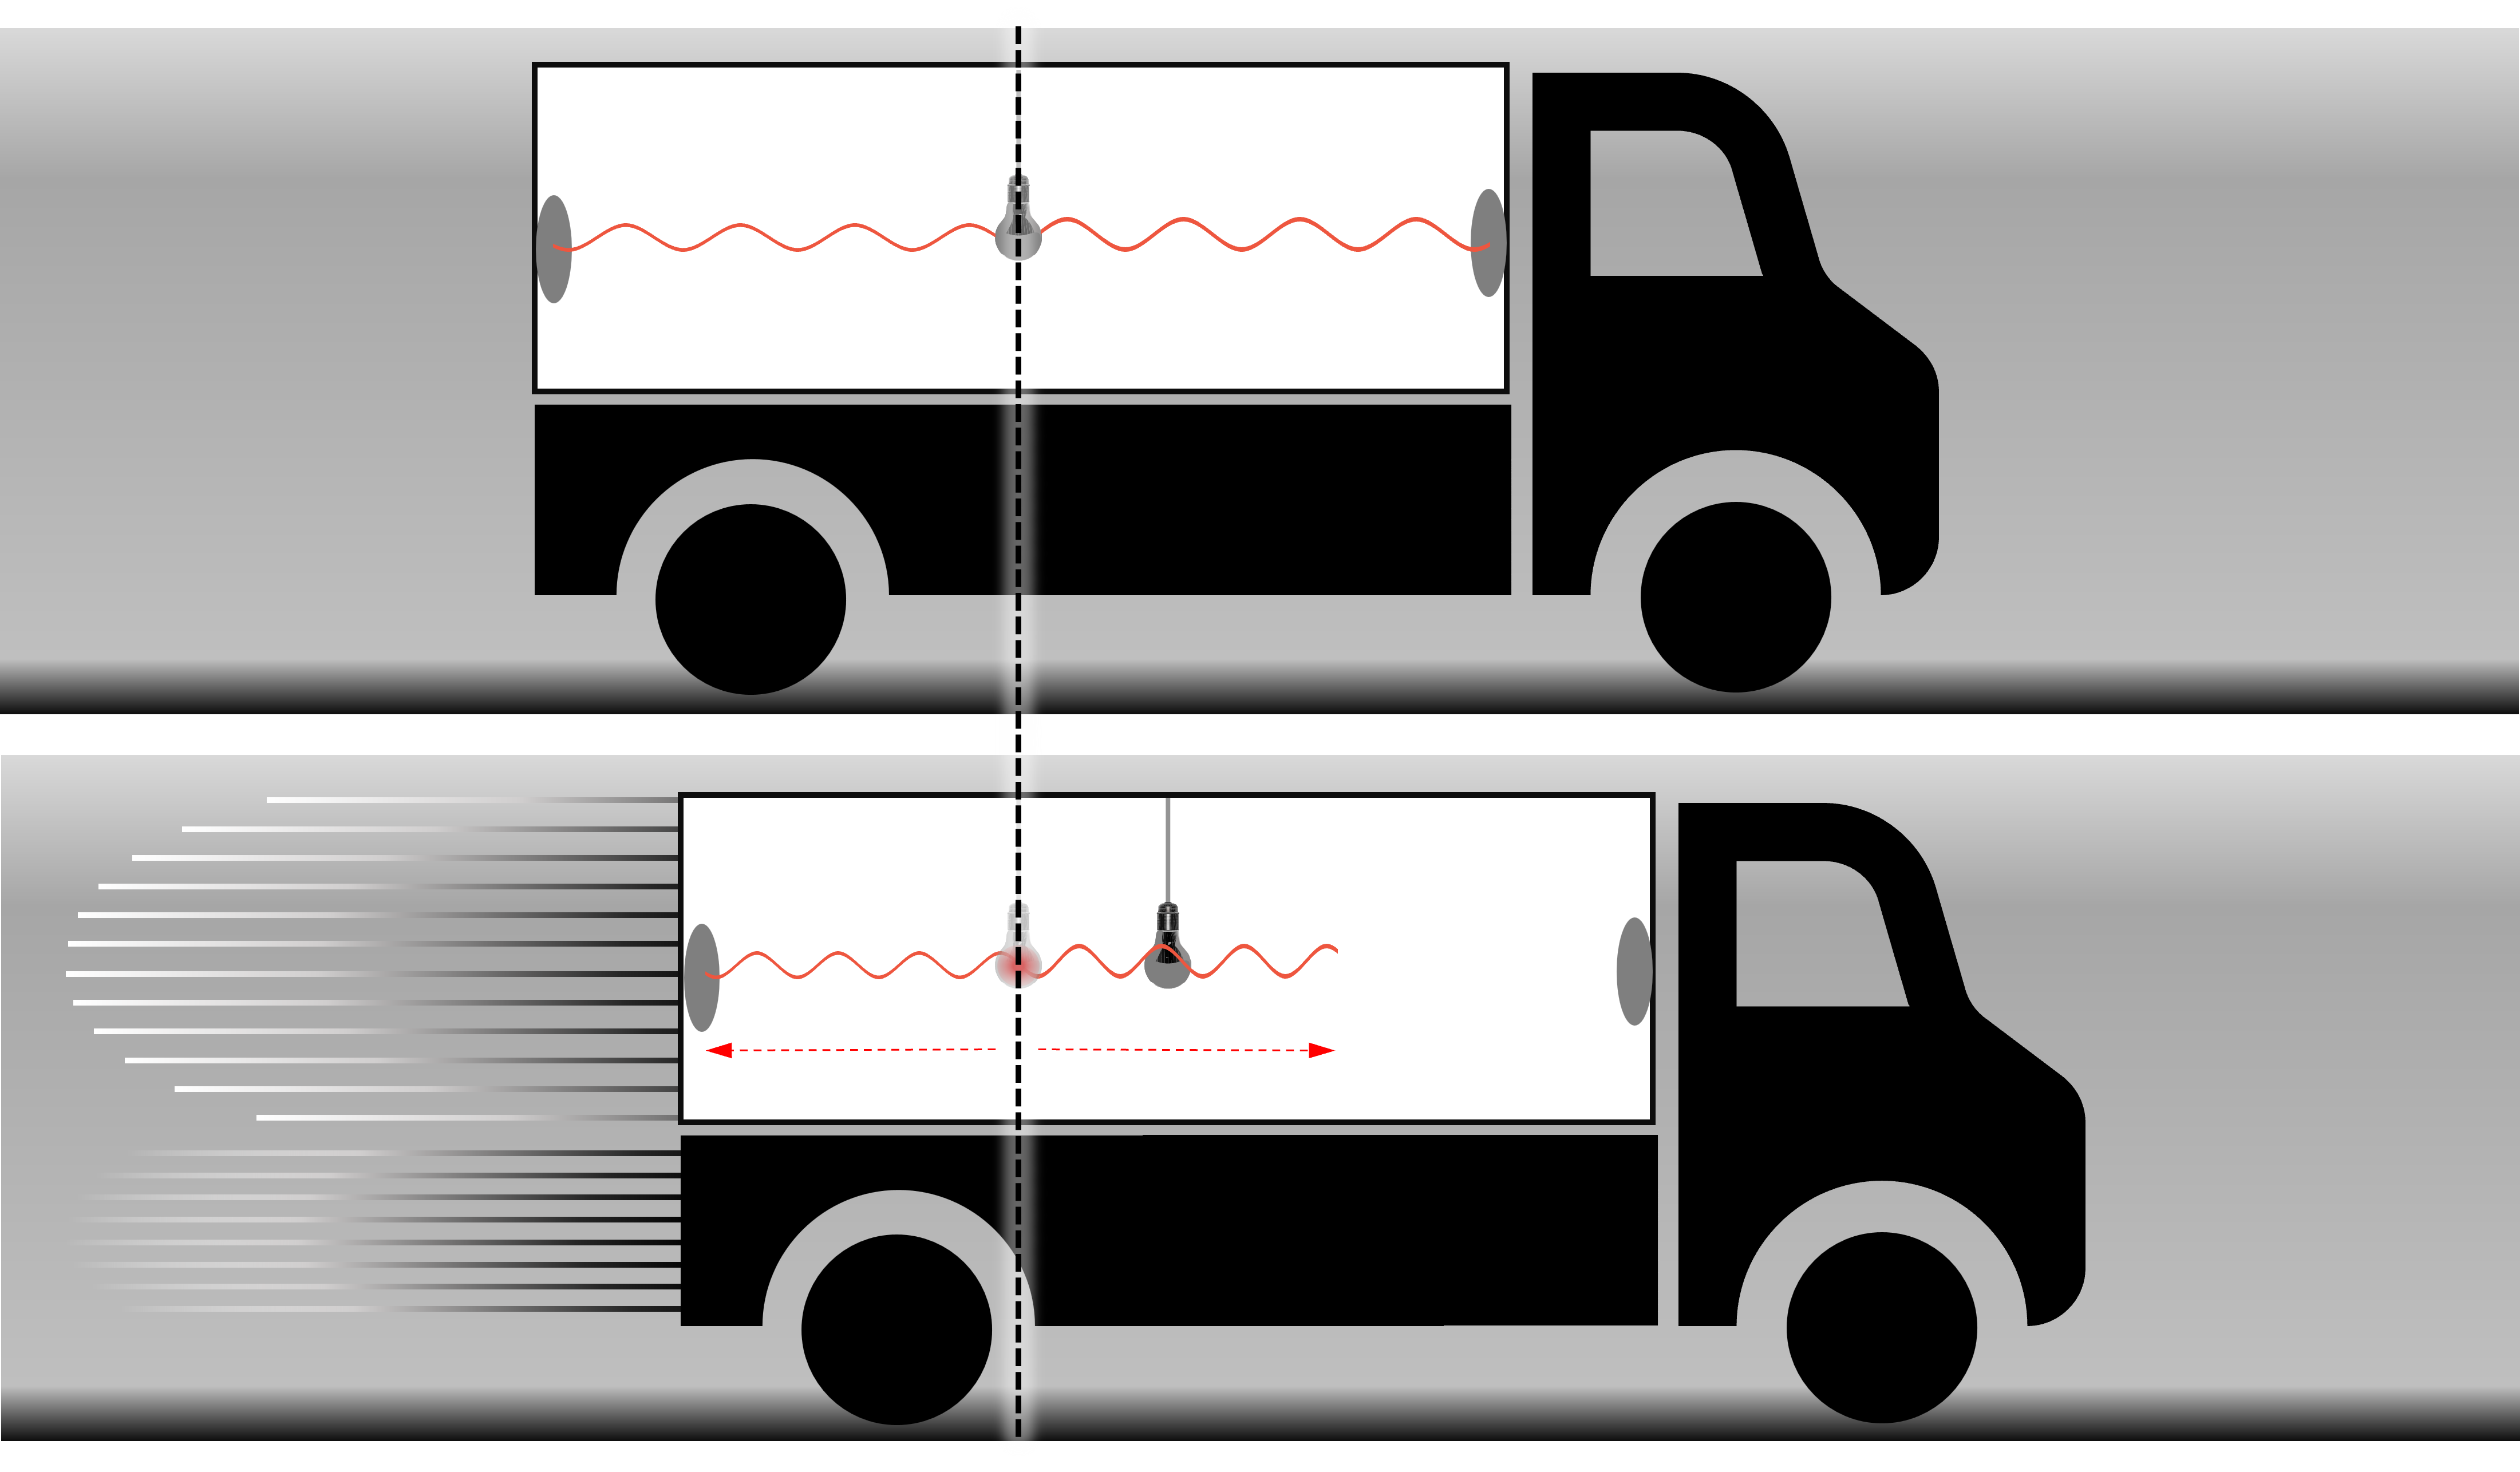
\includegraphics[width=8cm]{lorry_simul.png}
    \caption{A diagram showing how the two \protect\hyperlink{def-event}{event}s of light reaching the two walls of the truck are \protect\hyperlink{def-simultaneity}{simultaneous} in one frame but happen at different times in another, due to truck's movement in the second frame and the speed of light remaining the same.}
    \label{fig: truck simultaneity}
\end{figure}

Let us imagine a truck in its \hyperlink{def-proper-frame}{rest frame}, with a light bulb in the middle and mirrors on the front and back walls, now if the light bulb gives off a pulse of light, the light will travel from the centre of the truck to reach the mirrors \hyperlink{def-simultaneity}{simultaneously} and back to the light bulb also \hyperlink{def-simultaneity}{simultaneously}. 
But the \hyperlink{def-observer}{observer} on the road watching the truck drive past will see the light bulb \hyperlink{def-simultaneity}{simultaneously} emit light in both directions and also \hyperlink{def-simultaneity}{simultaneously} return to the bulb again. However, to do this the light reflects off each wall's mirrors at different times in this frame as shown in the diagram. This is because the speed of light is the same for both directions but the truck is moving, meaning the back of the truck is moving towards where the bulb was when the pulse was emitted making the distances travelled shorter, and due to the front wall moving away from it, the light travels a longer distance to get to the front wall. Due to this and the speed of light being the same in both \hyperlink{def-Reference-frame}{reference frame}s, the \hyperlink{def-observer}{observer} on the road will see the light hit the mirrors at different times.
So, times of \hyperlink{def-event}{event}s (like when the light reaches either mirror) are different for \hyperlink{def-observer}{observer}s in different \hyperlink{def-Reference-frame}{reference frame}s, there is no one true order of \hyperlink{def-event}{event}s, e.g. an \hyperlink{def-observer}{observer} in a faster moving truck moving in an opposite direction would see the light reach the front wall first.
However for all \hyperlink{def-observer}{observer}s the light will return to the central light bulb \hyperlink{def-simultaneity}{simultaneously}. If two \hyperlink{def-event}{event}s happen in the same position at the same time (i.e. the light returning to the centre of the light bulb \hyperlink{def-simultaneity}{simultaneously}) then this happens \hyperlink{def-simultaneity}{simultaneously} in all frames of reference. 

I have left out any mention of \hyperlink{def-length-contraction}{length contraction}, which will be introduced in the next section, and why it needs to be equal in both directions from light bulb, i.e. for the light to \hyperlink{def-simultaneity}{simultaneously} return to the light bulb they need to maintain equal distances of the walls from the central light bulb.


%███████████████████████████████████████████████████████████████████
\subsection{Length Contraction}

\begin{figure}[H]
\centering
       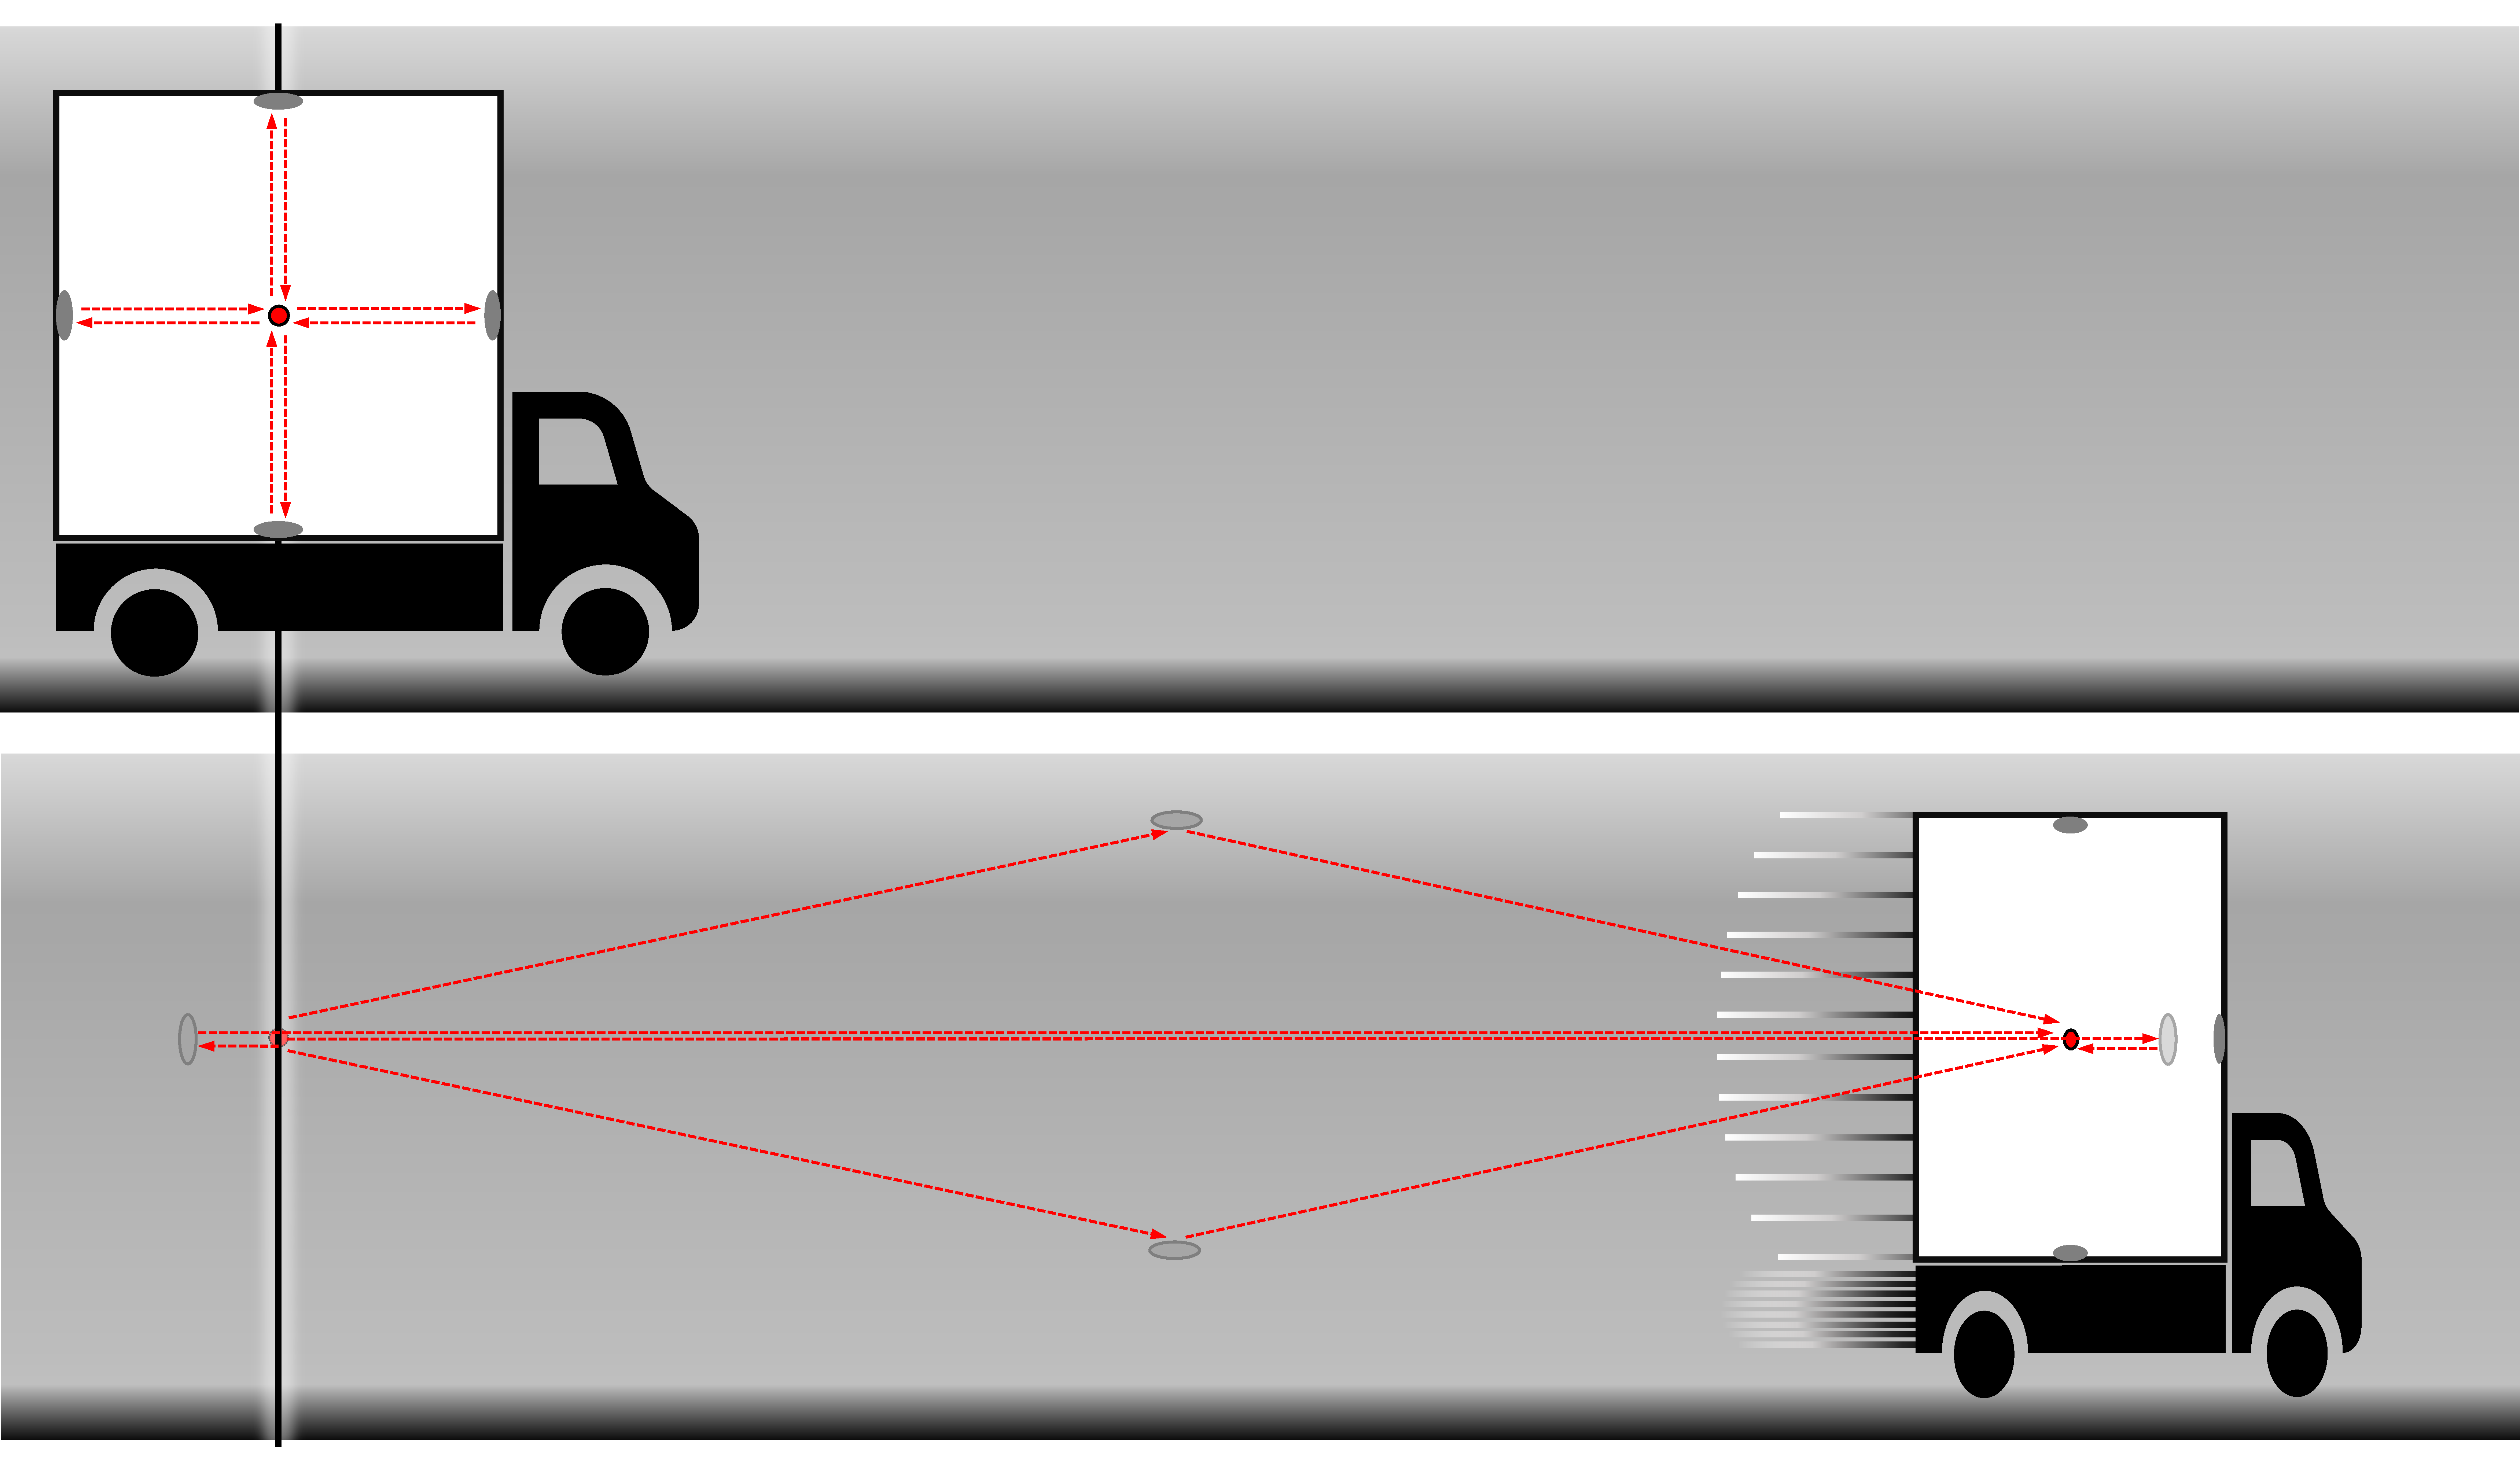
\includegraphics[width=8cm]{Full_Lorry_Transform.pdf}
    \caption{A diagram, showing a truck with a square container in it's \protect\hyperlink{def-proper-frame}{rest frame} (top), emitting light from a central bulb in the four directions, with all light being reflected by the mirrored sides back to the centre. In the second frame with the truck now moving (bottom) we see the truck 's length contracted and what the light paths would be in this frame}
    \label{fig: full truck transform}
\end{figure}


If we have a truck in its \hyperlink{def-proper-frame}{rest frame} with square container with light emitted in all four directions from the centre, so that it will bounce off the mirrored sides of the truck and return to the centre \hyperlink{def-simultaneity}{simultaneously}. we require that in the moving frame they also all return to the centre \hyperlink{def-simultaneity}{simultaneously}, as multiple \hyperlink{def-event}{event}s that happen at a single point \hyperlink{def-simultaneity}{simultaneously} in one frame, must happen \hyperlink{def-simultaneity}{simultaneously} in all other frames. This time between light being emitted and absorbed will be the \hyperlink{def-time-dilation}{dilated time}, that was described in the \hyperlink{def-time-dilation}{time dilation} section. 

To achieve this \hyperlink{def-simultaneity}{simultaneity} in the return of the light to the bulb, the length of the path of light in each direction has to be the same (as its speed is same in all directions), we can work out the length of the upward path from the \hyperlink{def-time-dilation}{time dilation} section, and this is the length the path needs to be in the horizontal directions as well, the paths can only have this length if the truck length is contracted when moving, the exact amount of contraction can be worked geometrically. And it turns out that the ratio of the increase in the amount of time that passes before light is reabsorbed is inversely proportional to the amount the truck is contracted in the direction of its movement.

i.e. time passes by a factor slower in the moving frame, and the change in distances in the direction of movement are inversely proportional to the same factor.

The reason that we do not worry about contraction in the distance between the floor and ceiling mirrors, will be explained in a later section.

%... the faster you go the closer things are in that frame, so it would take shorter an shorter amounts of time to get to places the closer you get to the speed of light (is this true)



%██████████████████████
\subsubsection{3 car system way of explaining length contraction (may delete)}


\begin{figure}[ht]
\centering
       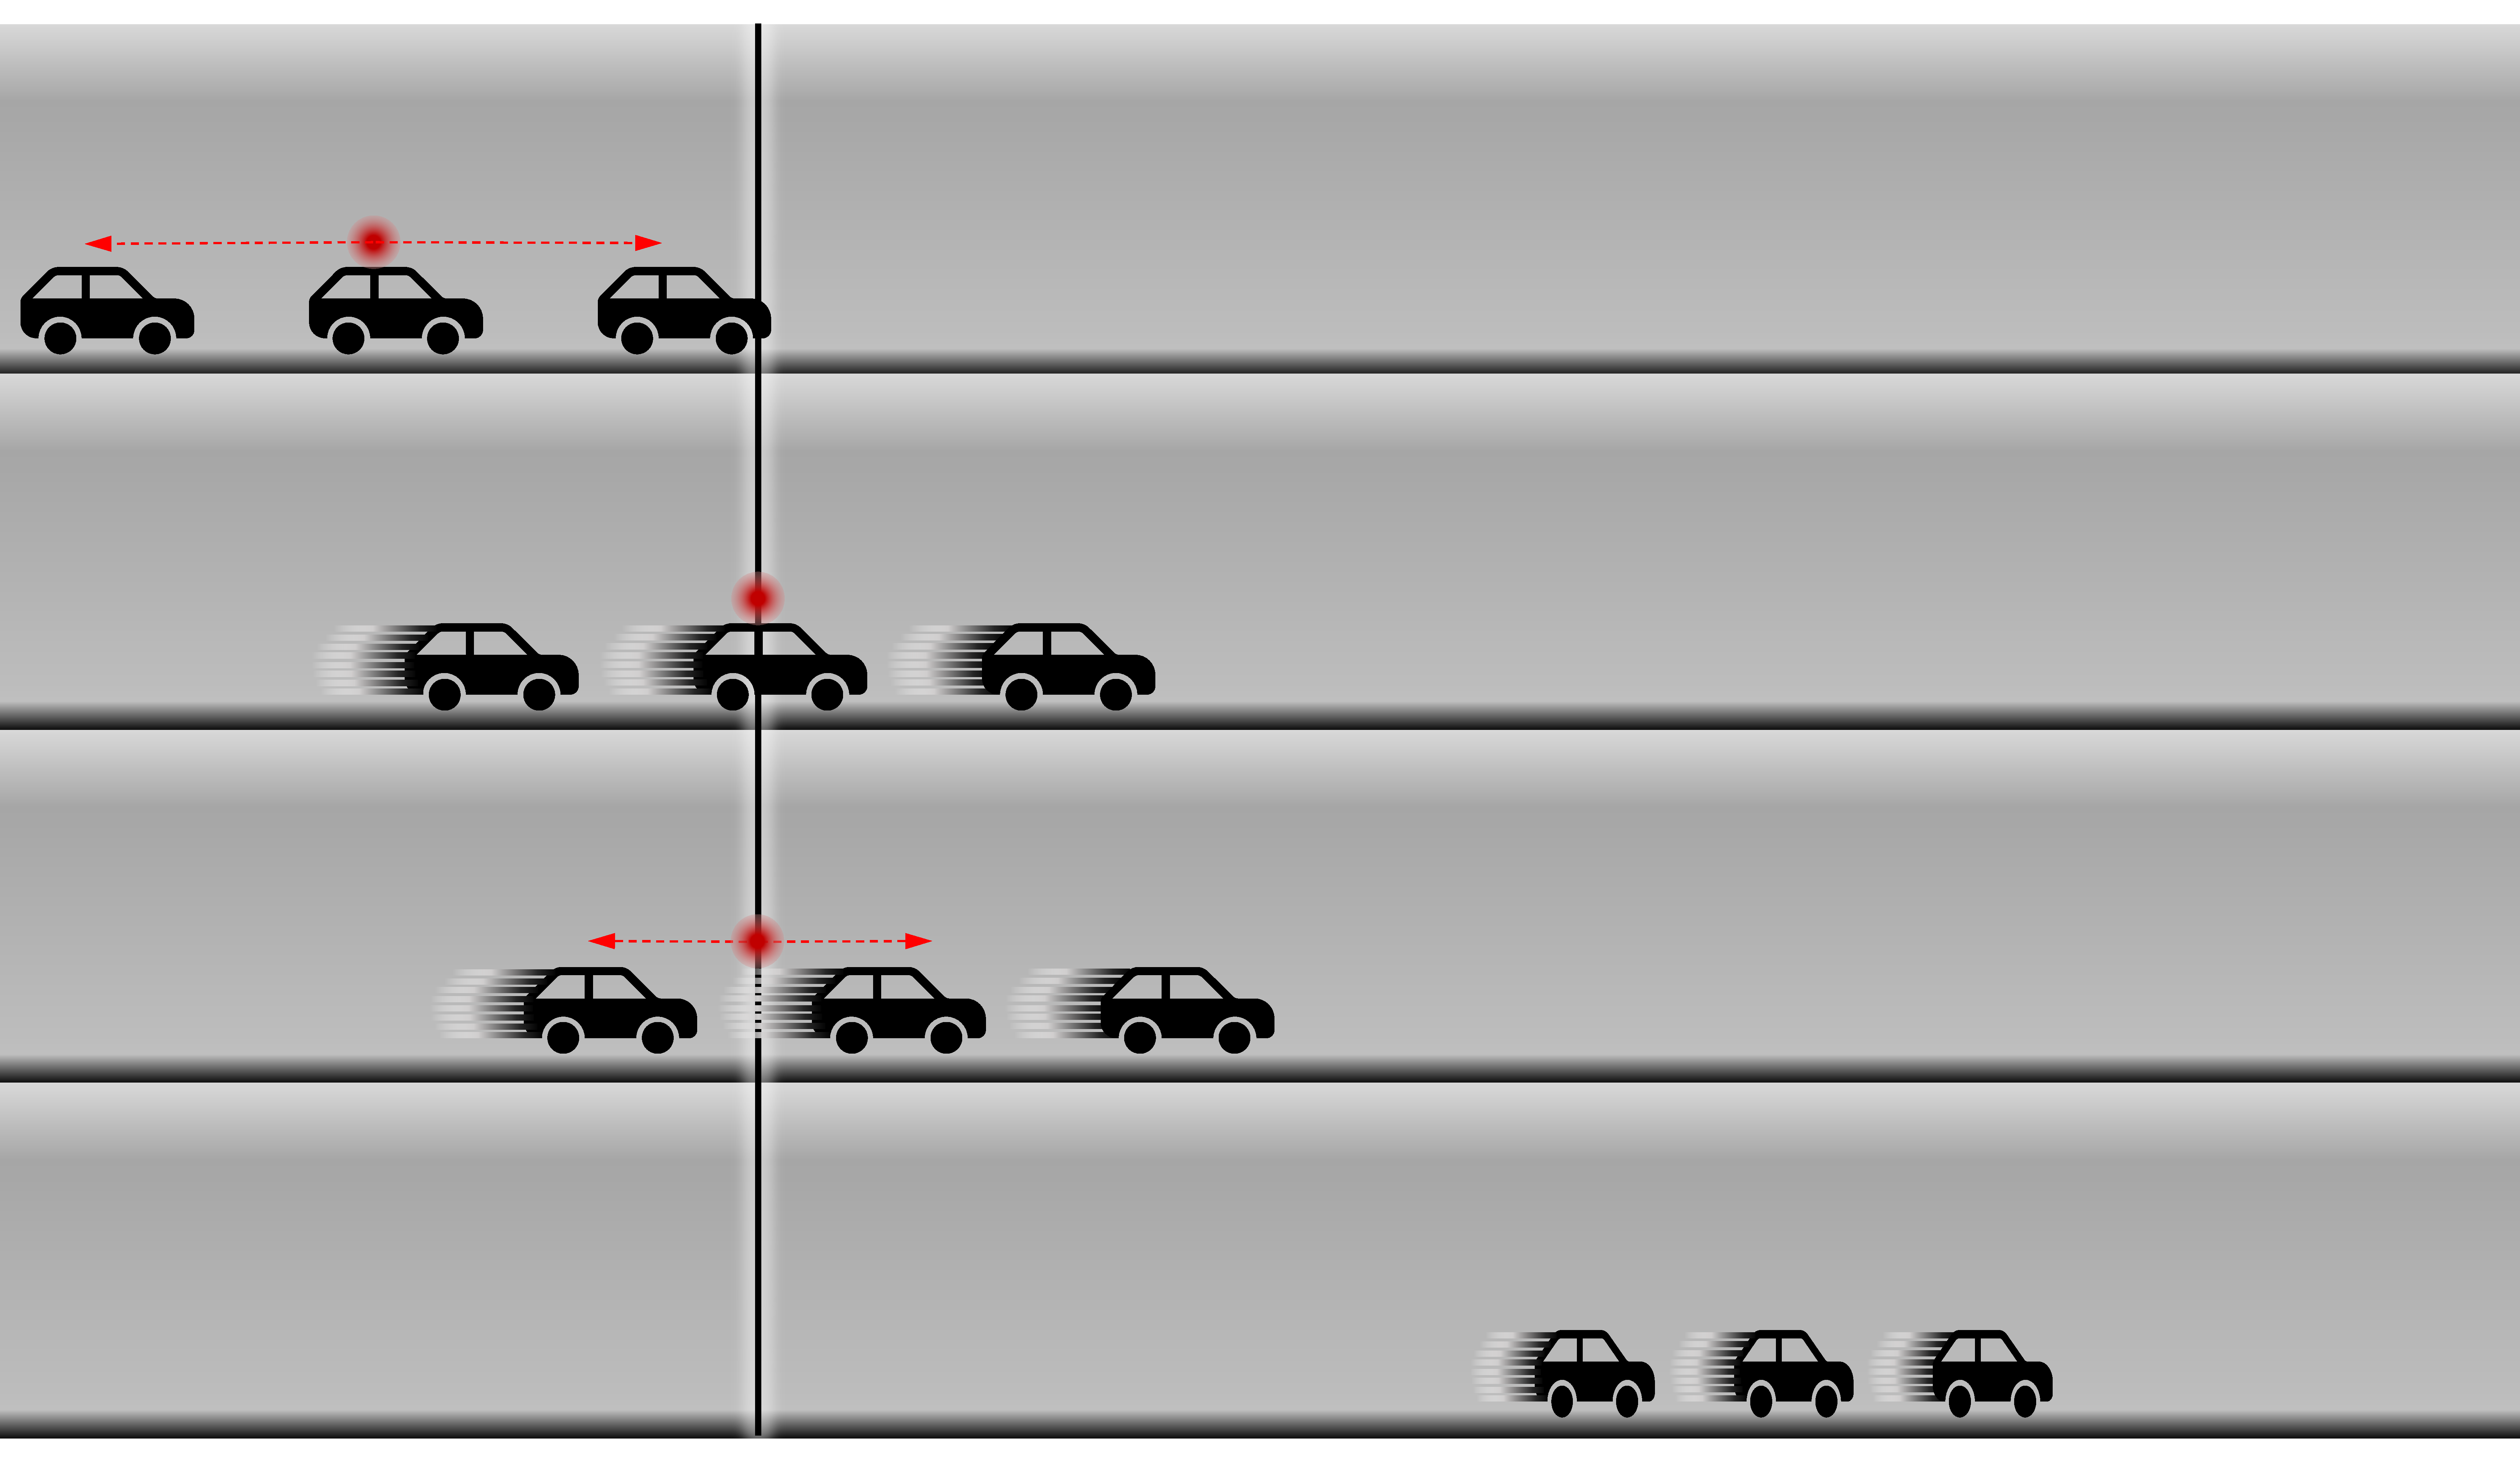
\includegraphics[width=8cm]{cars.pdf}
    \caption{Diagram that illustrates an experiment with three cars initially at rest and equally spaced on a road. The middle car emits light that reaches the front and back cars \protect\hyperlink{def-simultaneity}{simultaneously}, triggering all cars to accelerate for a predetermined amount of time. Now another light is emitted from the middle car after the acceleration has finished, the road \protect\hyperlink{def-observer}{observer} sees the light reach the back car first, as it is moving towards where the light had been emitted, this causes it to begin accelerating before the front car. This results in the cars being closer together after acceleration, demonstrating Lorentz \protect\hyperlink{def-length-contraction}{length contraction}, However, to the car \protect\hyperlink{def-observer}{observer}, the distance between the cars remains unchanged from the initial distances.}
    \label{fig: cars}
\end{figure}

Say we have 3 cars that are equally distanced and at rest on the road, the middle car sends out a pulse of light that reaches the front and back car at the same time to the road \hyperlink{def-observer}{observer} and the \hyperlink{def-observer}{observer}s in the car, when it reaches them both, all the cars accelerate for a predetermined fixed amount of time, so that after this acceleration period the cars are now moving but still equally spaced relative to the \hyperlink{def-observer}{observer}s in the cars and the \hyperlink{def-observer}{observer} on the road. As for all \hyperlink{def-observer}{observer}s the light reaches the front and back cars at the same time. 

now if we do this a second time and the middle car releases another pulse, in the frame of the \hyperlink{def-observer}{observer}s in the cars: again the front and back drivers receive the pulses at the same time and accelerate, and again after the acceleration they have the same equal distance between the cars. But for the \hyperlink{def-observer}{observer} on the road, they see the back car receive the signal first as that car is moving towards the point where the light pulse was emitted and the front car is moving away from it. This would mean the back car would start accelerating first to get to the final constant velocity and get closer to the front car before the front car begins to accelerate, hence the cars end up closer together after all of this. The \hyperlink{def-observer}{observer}s in the car and the road \hyperlink{def-observer}{observer}, do not agree with what the distances between the cars is. This contraction of length between cars, in the frame in which the cars are moving, is called Lorentz \hyperlink{def-length-contraction}{length contraction}, which means that objects that are moving faster become shorter, the distances between the objects also become shorter.



%███████████████████████████████████████████████████████████████████
\subsection{No Width Contraction} \label{width contraction}

\begin{figure}[H]
\centering
       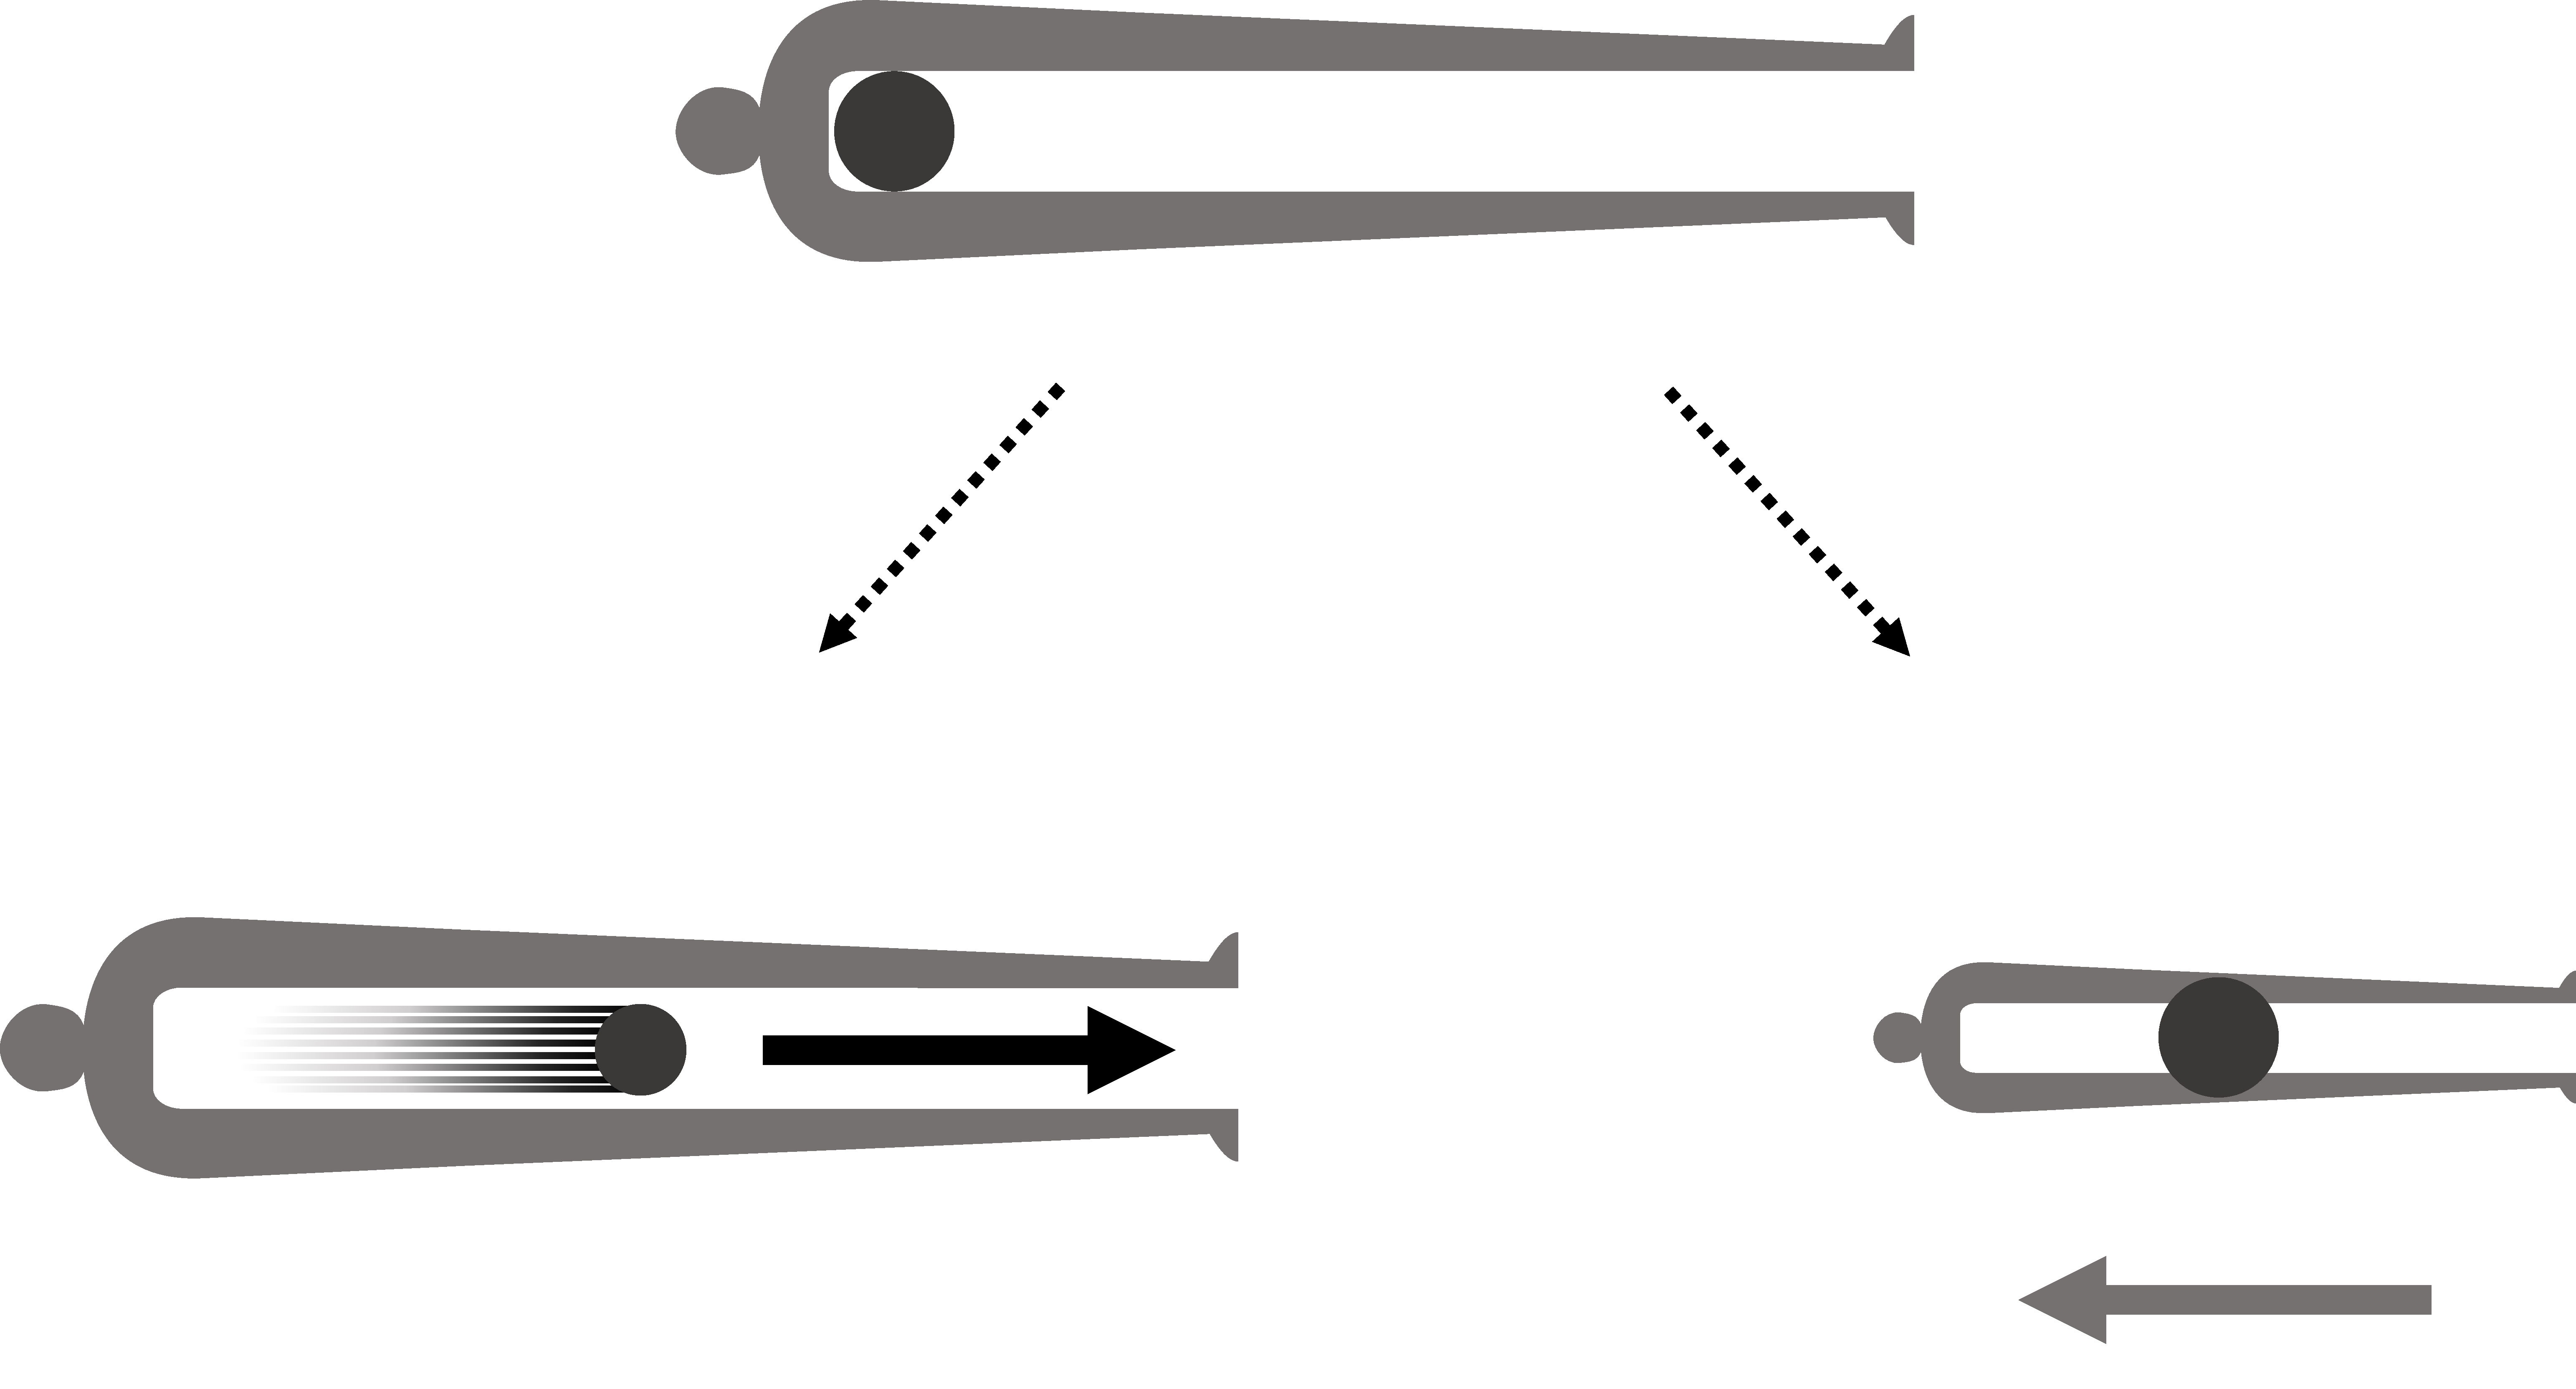
\includegraphics[width=8cm]{Cannon_Balls.pdf}
    \caption{A diagram showing why there must not be contraction in perpendicular direction to frames relative motion. The top figure shows a ball and cannon at rest, the bottom figures show the cannon ball being fired in the frame of cannon (left) were the moving ball has a contracted width, and shows the frame of the ball (right) were now the canon is now moving and has a contract width, with the ball at rest being the same size, both frames would contradict each other, if there was a change in width of moving objects, as the walls of the cannon and the balls surface would overlap in one frame and not be touching in the other. So we require that there is no change in size perpendicular to the movement of the object.}
    \label{fig: Cannonball}
\end{figure}


%Suppose we have a ball at rest in a pipe such that the ball just touches the inner circumference of the pipe, if we were to now make the ball move we would have it Lorentz contracted along the direction of the movement, but if we also had it contract perpendicular to the direction of movement then in the rest frame of the pipe we would have the ball smaller such that it no longer was touching the inner pipe, but if we changed to the frame of the ball it would be the pipe that was moving and we would expect the pipe to contract and be smaller than the ball (so that the ball would get stuck), so in the two different frames we would have two contradictory outcomes, but we should be able to go from one frame to the other and not have these contradictions, so to have this we require that there is no change in size perpendicular to the movement of the object.


%███████████████████████████████████████████████████████████████████
\section{Doppler Effect}

\begin{figure}[H]
\centering
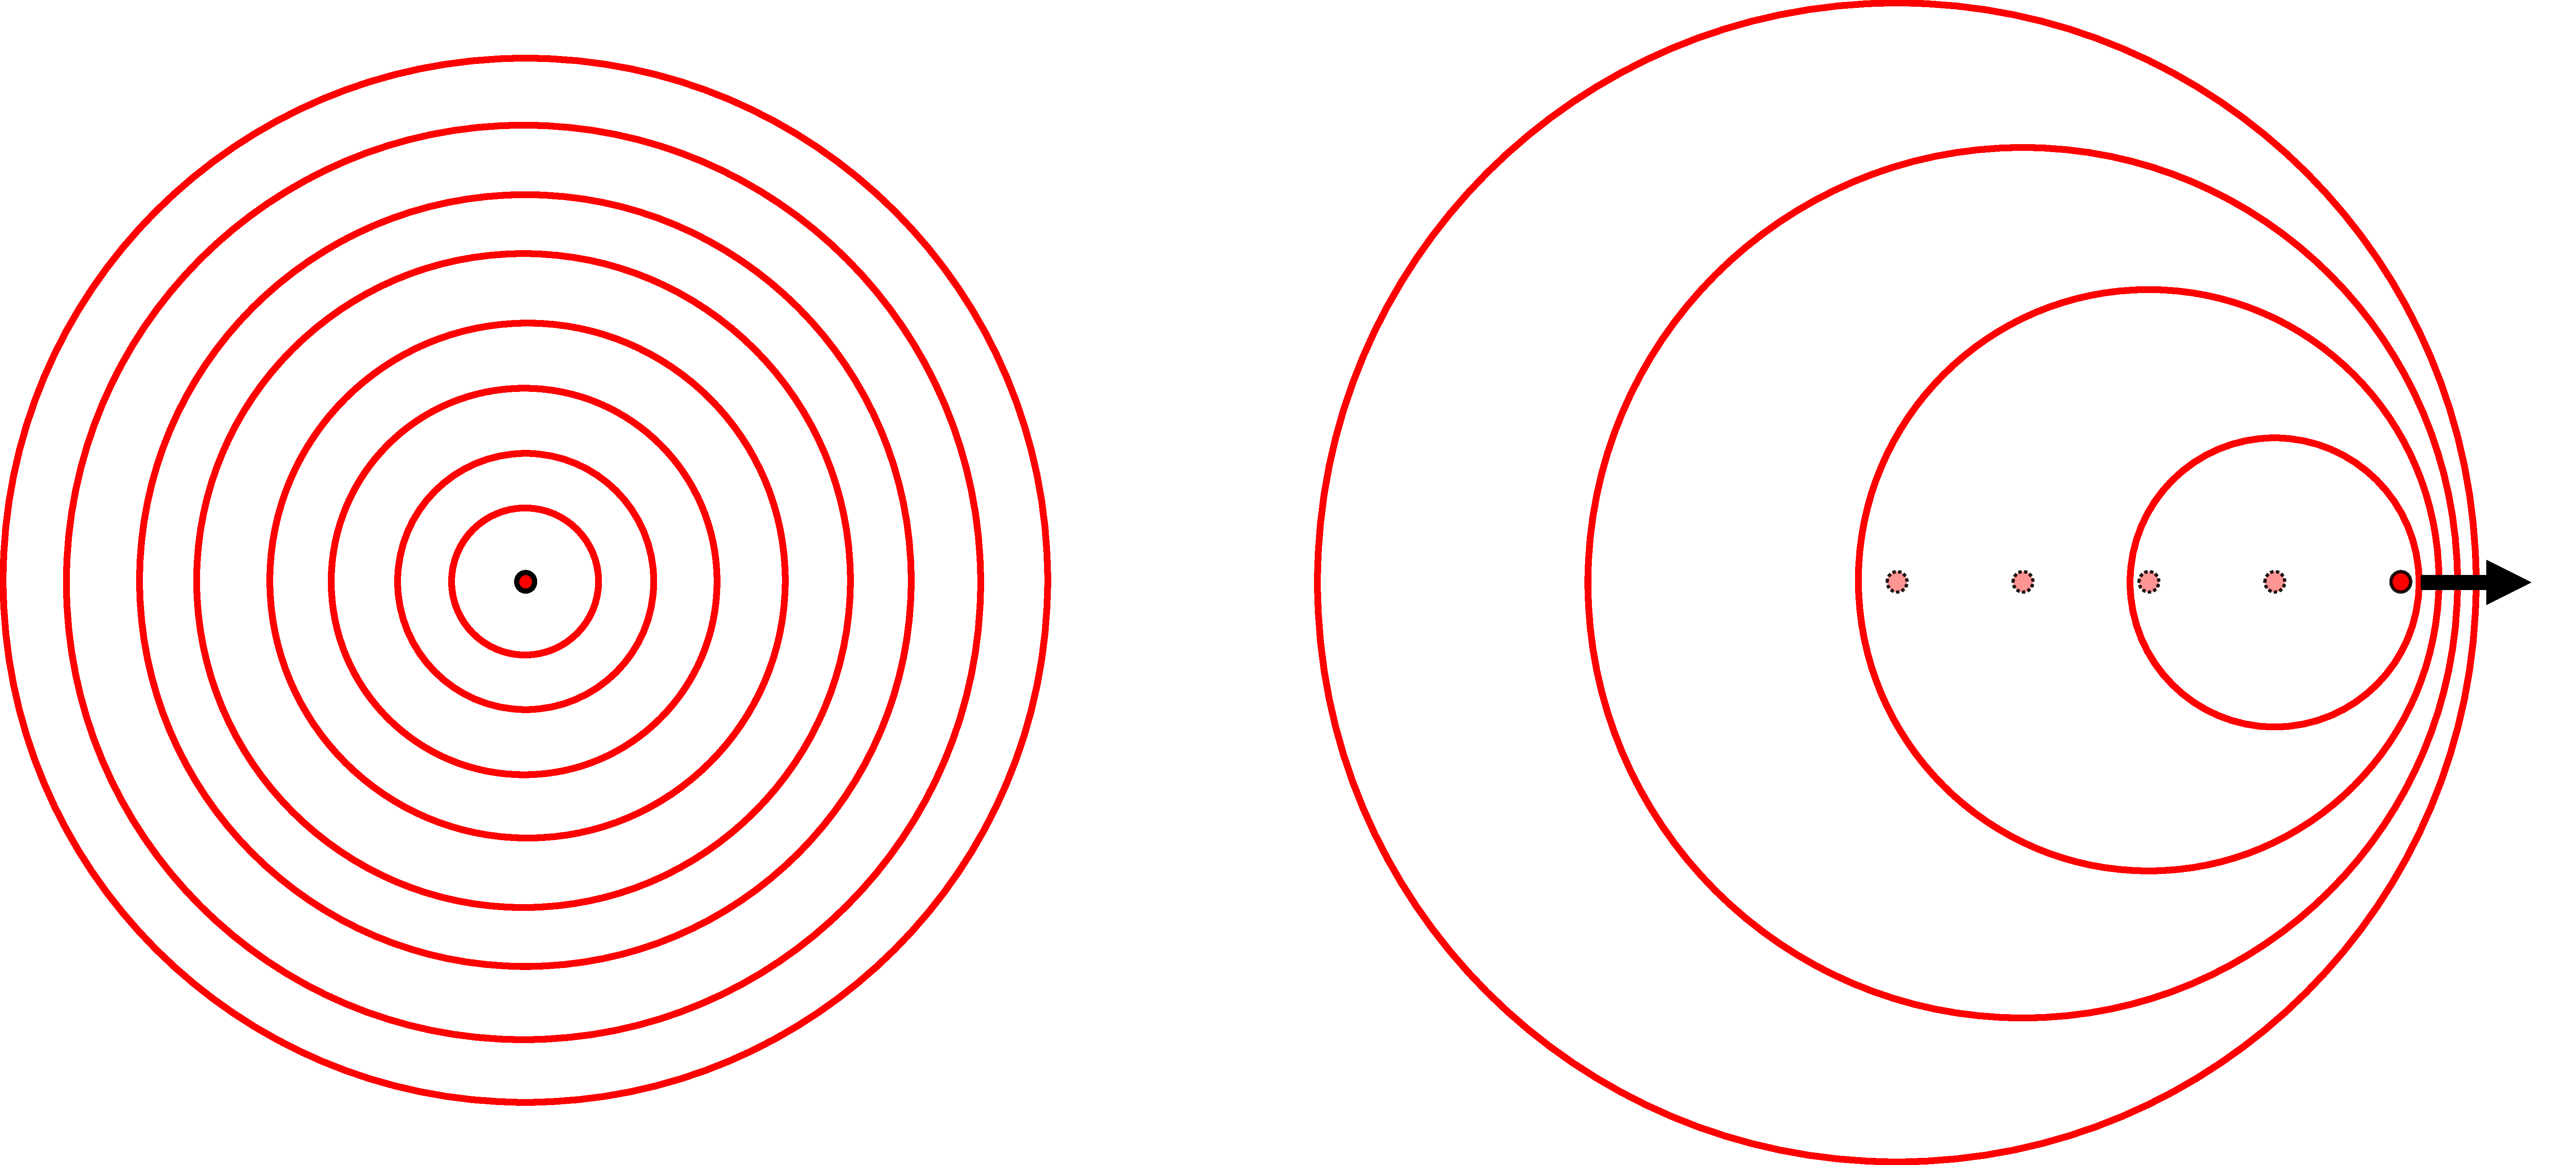
\includegraphics[width=10cm]{Doppler.pdf}
    \caption{A diagram showing (left) a central source at rest emitting several circular pulses of light with equal time between each pulse, (right) the same source in a frame where it is now moving and emitting circular pulses of light, but each subsequential pulse is emitted from a different position as the source is moving, marked by a faded dot}
    \label{fig: doppler effect intro}
\end{figure}

If we have a source at rest, emitting circular pulses of light with equal times between each pulse, we will have concentric circular pulses in this frame, but if we move to a frame where the source is now moving to the right, each circular pulse is now being emitted from a different position as the source is moving. Due to the source moving, each pulse will be emitted closer to the right hand side of the previous pulses, creating a bunching up of the pulses (increase in frequency) in the direction of movement and a spreading out (decrease in frequency) of the pulses in the opposite direction, that is what happens in the classical version of the \hyperlink{def-doppler-effect}{Doppler effect}, that you will notice that an ambulance or police car sounds different driving towards you and when driving away, this is due to the bunching up of the sounds waves in the direction of the moving vehicle. In special relativity, we also have to take the \hyperlink{def-time-dilation}{time dilation} of the pulses into account, as there will be a longer time between each subsequential circular pulse, Due to perceived time moving more slowly for objects moving relative to the \hyperlink{def-observer}{observer}, this has a decreasing effect on the frequency in all directions, but directly in the direction of movement of the source this is outweighed by the frequency increase from the previous bunching up effect. Since the energy of the light is proportional to the frequency it is increased in the direction of motion of the source due to the \hyperlink{def-doppler-effect}{Doppler effect}s and decreased in the opposite direction.

One thing not mentioned yet in this picture so far is how the light is also effected by what is called the \hyperlink{def-aberration}{aberration}, which is the change in the direction of each part of the emitted light pulse, which leads to light not being circularly symmetric in each of the spherical pulses, which will be explained in the next section.

%███████████████████████████████████████████████████████████████████
%███████████████████████████████████████████████████████████████████
\section{Aberration}

The picture painted of the \hyperlink{def-doppler-effect}{Doppler effect} in the previous section has yet to show the effect on the angular distribution of the light in each of the spherical pulses. Here we will show that there is also a higher concentration of light in the direction of the source's movement, as shown in Figure \ref{fig: truck aberrated}.


\begin{figure}[htbp]
\begin{subfigure}{.49\textwidth}
\centering
       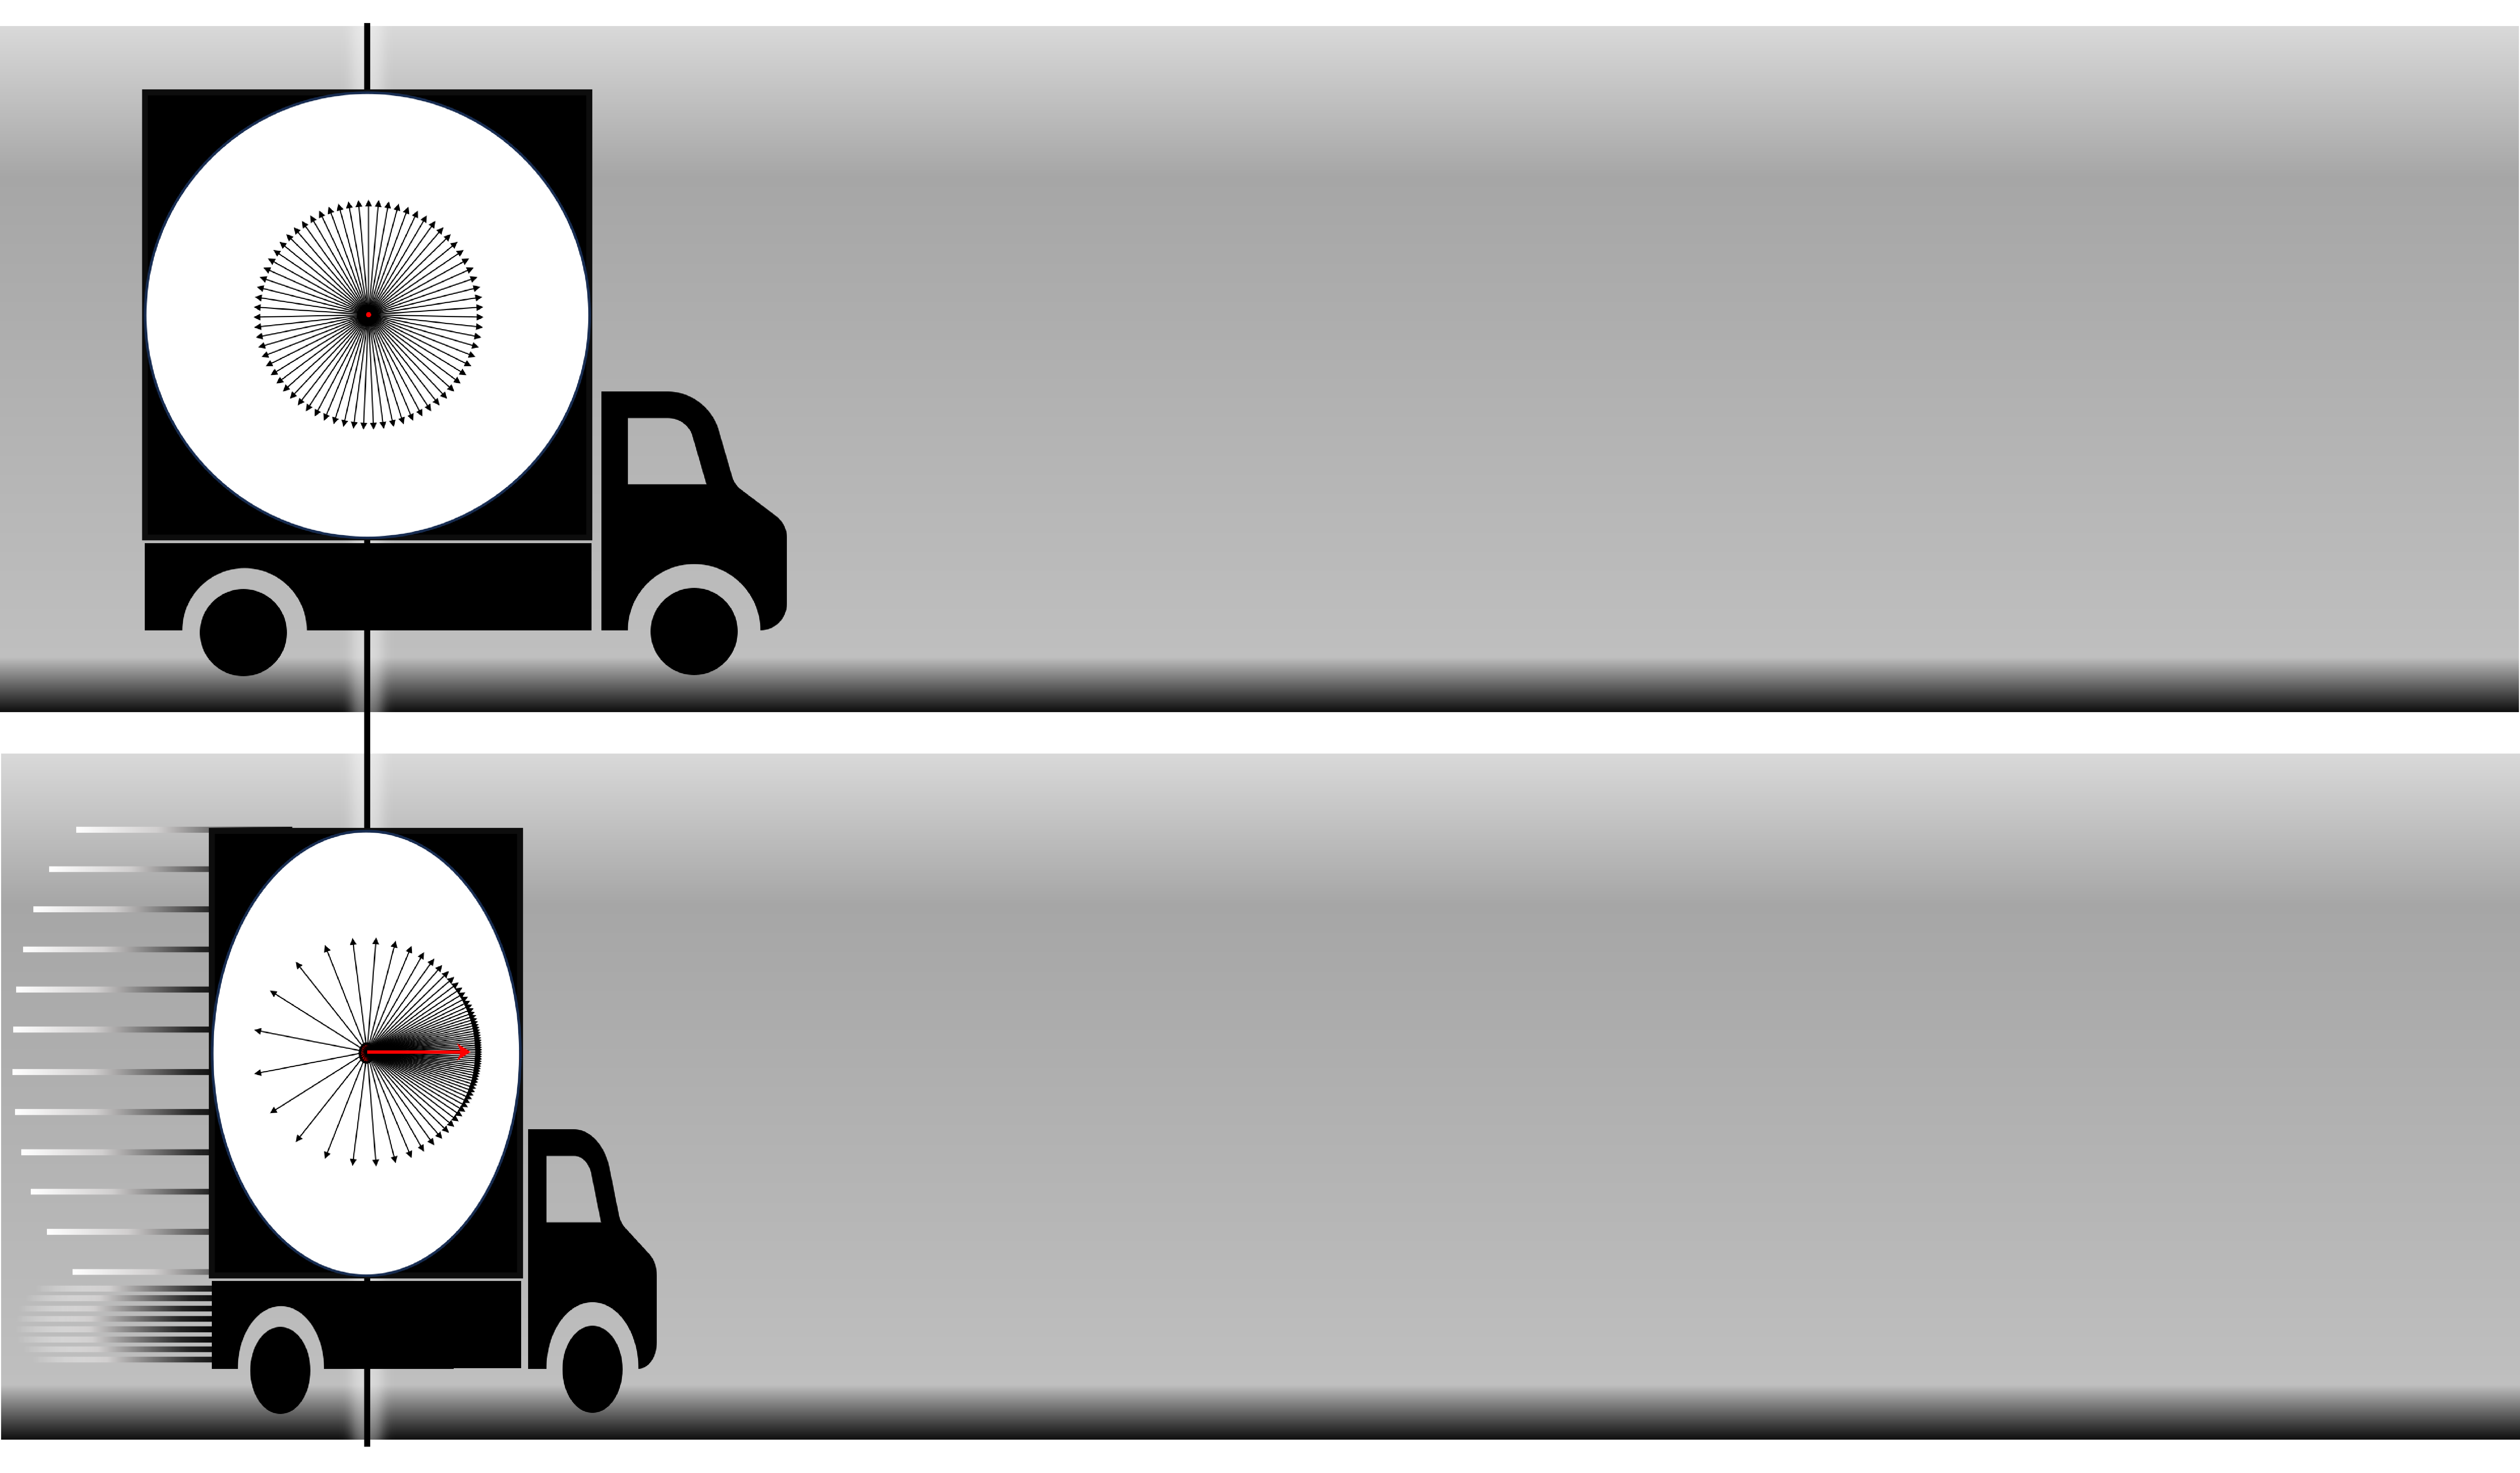
\includegraphics[width=5cm]{Aberrated_lorrys_1.pdf}
    \caption{Pulse emitted}
    \label{fig: truck aberrated 1}
\end{subfigure}
\begin{subfigure}{.49\textwidth}
\centering
       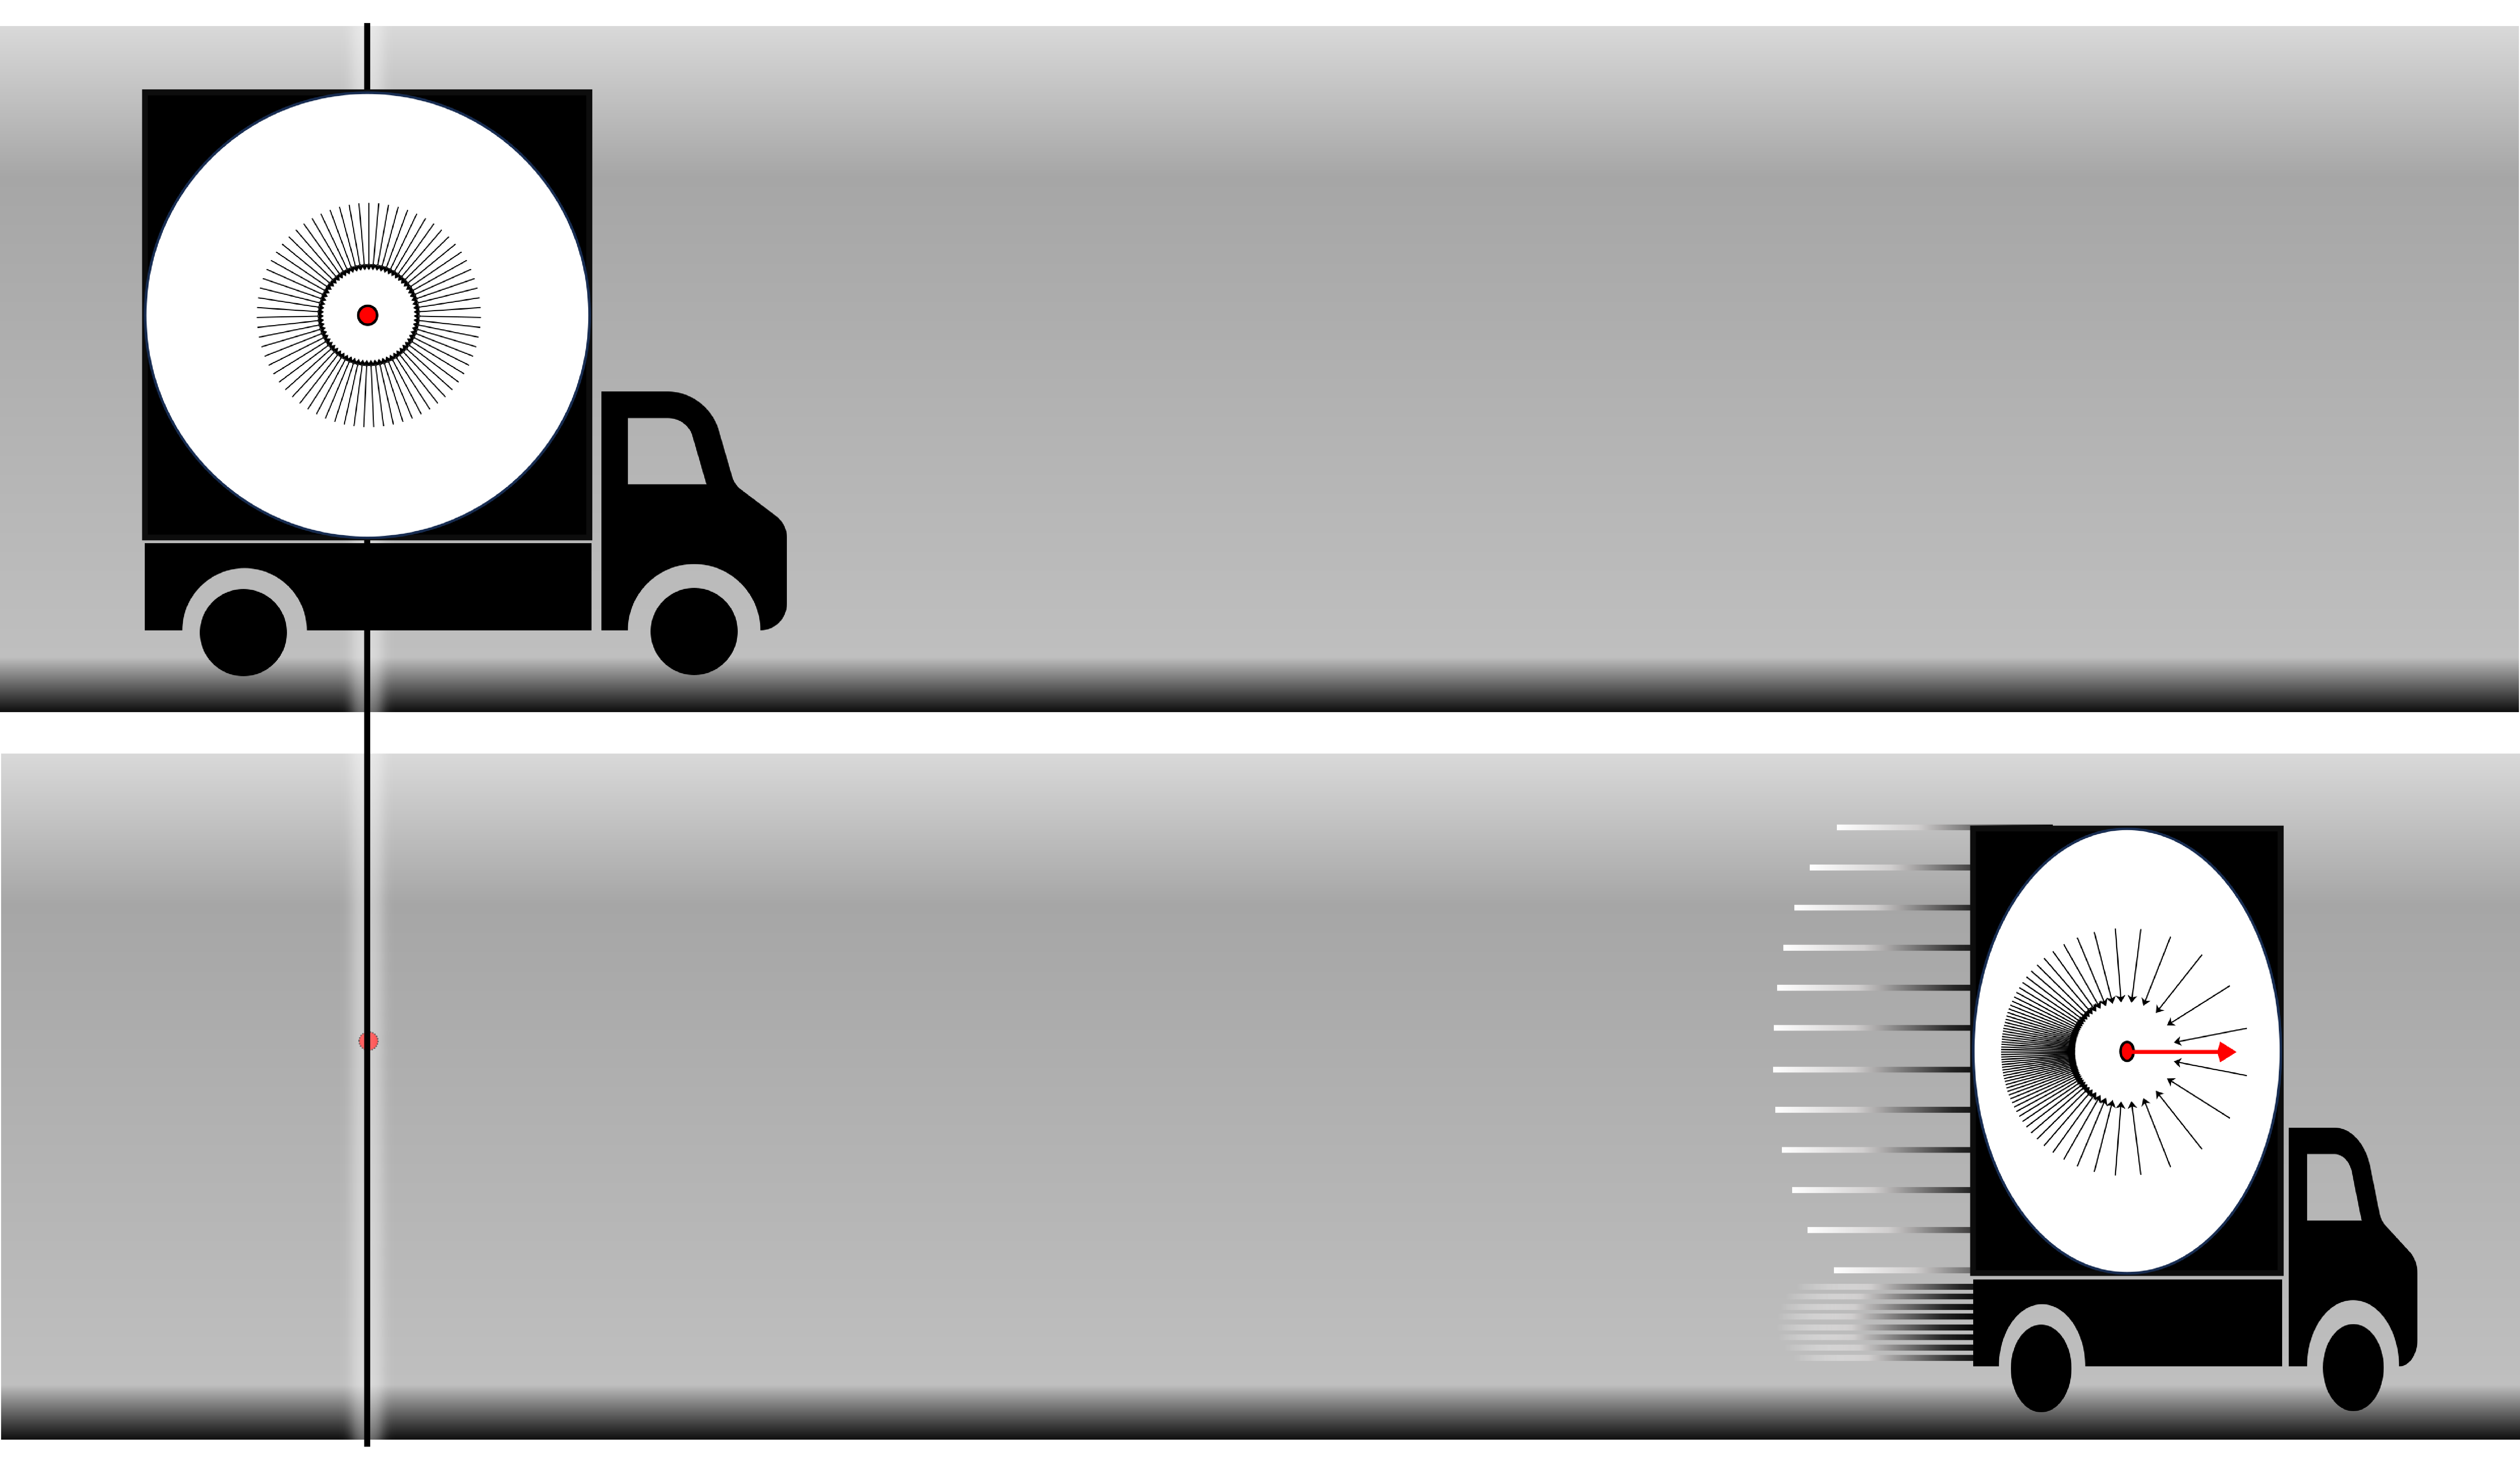
\includegraphics[width=5cm]{Aberrated_lorrys_2.pdf}
    \caption{Pulse absorbed}
    \label{fig: truck aberrated 2}
\end{subfigure}
\caption{Two diagrams of a truck with a spherical container in two different frames, a light pulse is emitted from the centre of the container (left) and reflected back by the mirrored wall to be absorbed in the centre again (right), the truck in its \protect\hyperlink{def-proper-frame}{rest frame} (top of both figures) shows a evenly distributed light outward pulse, but in the frame with the moving truck (bottom of both figures) the emitted light is now more concentrated in the direction of the truck , which is required to allow the light to be reflected and returned to the centre of the truck \protect\hyperlink{def-simultaneity}{simultaneously}.}
\label{fig: truck aberrated}
\end{figure}

\iffalse javascript{Aberration} \fi


With the help of the previous \hyperlink{def-length-contraction}{length contraction} section, let us imagine a truck with a spherical container with mirrored walls, a central bulb emits light in all directions, in the \hyperlink{def-proper-frame}{rest frame} all light reaches the spherical wall at the same time and returns to the center bulb \hyperlink{def-simultaneity}{simultaneously}.
Then in the moving frame we have the spherical container \hyperlink{def-length-contraction}{length contracted} and the light moving at the same speed but reflecting off the walls at different times, returning to the centre bulb simultaneous, for this to be true, the directions of the light have to be aberrated in the way shown in the diagram to allow for this \hyperlink{def-simultaneity}{simultaneous} return to the bulb.

From the diagrams you can see how light is aberrated when emitted from a moving source relative to its \hyperlink{def-proper-frame}{rest frame} and also when being absorbed by a source, the faster the source is moving, the more the direction of each part of the light pulse is aberrated.

If the speed of the source was to approach the speed of light, all emitted light would approach the direction of movement of the source, if the source was theoretically able to reach the speed of light, all light would be emitted in the direction of the source but also move at the same speed of the source, i.e. the source would move with the emitted light and it would not leave the vicinity of the source. Though the rate at which it emits it would also tend to zero. If a photon theoretically had mass and its influence of the gravitational force moved at the speed of light, then we would not be able to feel any gravitational effects outside the vicinity of it, due to all of its gravitational field being propagated in the direction of its movement and at the same speed as the photon.


Also in astrophysics it has to be taken into account that the earths view of the universe is distorted by \hyperlink{def-aberration}{aberration}, as shown in diagram ref{...} *** diagram of earths view of universe is distorted from the \hyperlink{def-aberration}{aberration} (example on wiki) ***

%███████████████████████████████████████████████████████████████████
%███████████████████████████████████████████████████████████████████
\section{Relativistic Beaming}

If we now take both the Doppler picture and the \hyperlink{def-aberration}{aberration} picture from the previous sections together, so that if we have a source that in its \hyperlink{def-proper-frame}{rest frame} is emitting a spherical pulse of light with evenly distributed angles. Then in a frame with the source now moving, we will have this spherical pulse's wavelength bunched up in the direction of movement (giving a change in the colour of the light), with the angular spread of the light at a higher concentration in the direction of the movement of the source.


\begin{figure}[htbp]
\begin{subfigure}{.49\textwidth}
\centering
       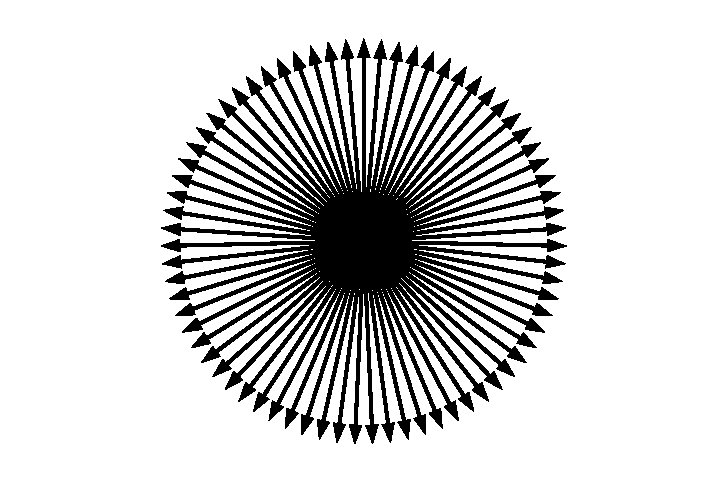
\includegraphics[width=5cm]{Rest_velocities.pdf}
    \caption{\hyperlink{def-proper-frame}{rest frame}}
\end{subfigure}
\begin{subfigure}{.49\textwidth}
\centering
       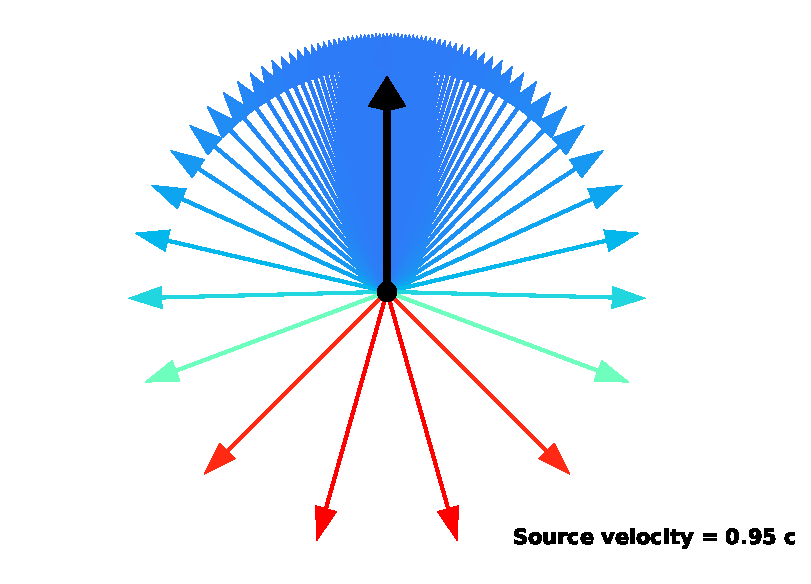
\includegraphics[width=5cm]{Aberrated_velocities.pdf}
    \caption{Moving frame}
\end{subfigure}
\caption{Outward pulse of light from source in a rest and moving frame}
\label{fig: outward pulse velocities}
\end{figure}

\begin{figure}[htbp]
\begin{subfigure}{.49\textwidth}
\centering
       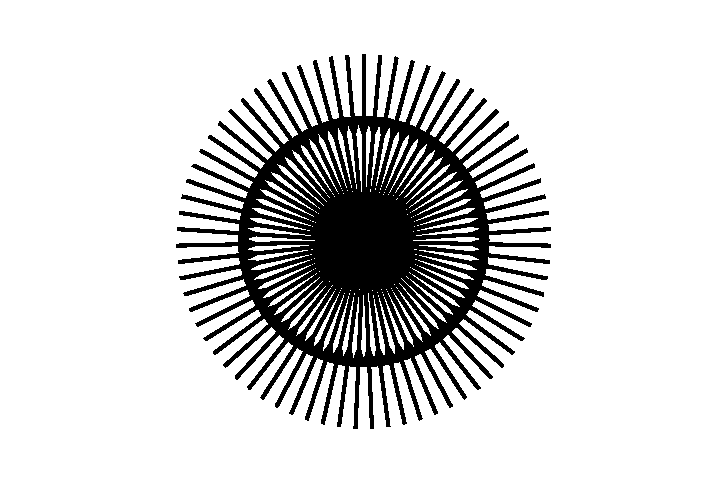
\includegraphics[width=5cm]{Rest_velocities_inwards.pdf}
    \caption{\hyperlink{def-proper-frame}{rest frame}}
\end{subfigure}
\begin{subfigure}{.49\textwidth}
\centering
       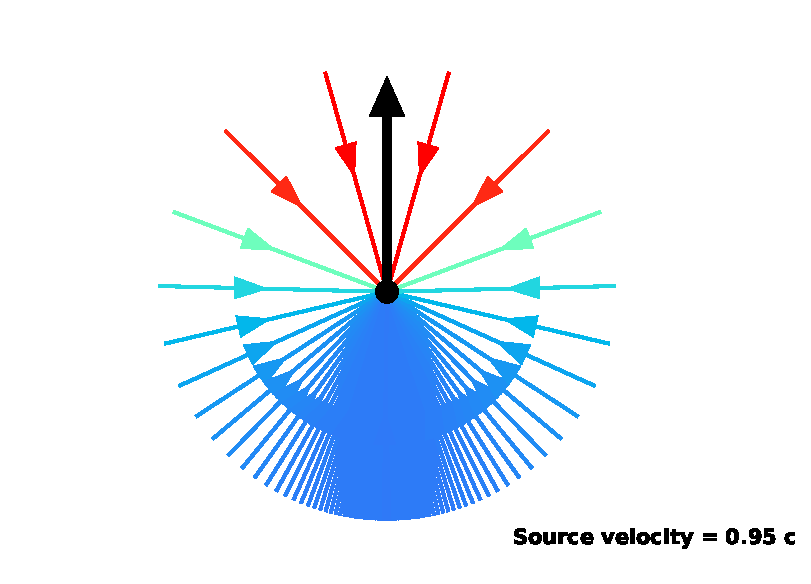
\includegraphics[width=5cm]{Aberrated_velocities_inwards.pdf}
    \caption{Moving frame}
\end{subfigure}
\caption{Inward pulse of light from source in a rest and moving frame}
\label{fig: Realivistic Beaming}
\end{figure}

%███████████████████████████████████████████████████████████████████
\subsection{Retarded Field}

If we were to have multiple pulses with a constant time between each pulse, and remembering that each pulses origin was from a point in the sources past position (the \hyperlink{def-retarded-position}{retarded position}  of the source), we can work out what the full view of all the pulses in the \hyperlink{def-proper-frame}{rest frame} is in the moving frame, shown in Figure \ref{fig: full field transformation 1}. From this we can work out the distribution and hence concentration of the light for any moving source relative to that of it at rest. 

\begin{figure}[ht]
\centering
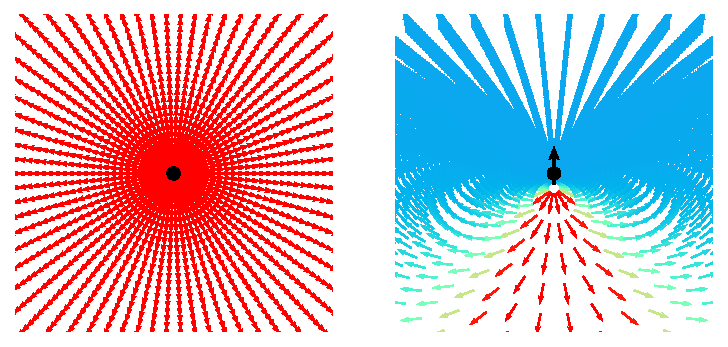
\includegraphics[width=10cm]{Still_Retarded_Field_Both_Frames.pdf}
    \caption{ A diagram showing multiple spherically pulses of light from a source at rest that have evenly distributed angles (left), and what it becomes in a corresponding frame where the source is moving (right)}
    \label{fig: full field transformation 1}
\end{figure}

%███████████████████████████████████████████████████████████████████
\subsection{Perceived vs Actual Speed}

Imagine that a ball one light year (the distance it takes light to travel in a year) away, is fired directly towards you. It will take one year for the first light from the oncoming ball to reach you. If the ball moves at three-quarters of the speed of light, the ball will hit you in four-thirds of a year (a year and four months) after it is fired. The last light from the ball will reach you just as the ball hits you. As you see it, the time between the first and last light from the ball is four months. During those four months, you will see the ball start at its initial position and travel a distance of one light year. So the ball appears to you to have been moving three times faster than light. This is just how it appears to the \hyperlink{def-observer}{observer} due to the delay in the light signal/the retarded view of the system, leading to latency on how the system is observed.
%*** from relativity vizualised book: 

This shows how important it is to take the delay in the light from objects into account when observing relativistic systems, this view is called the delayed/retarded view, i.e what we see now is objects in their past positions, and the further things are from you the further into the past we are currently seeing them. 

\begin{figure}[H]
\centering
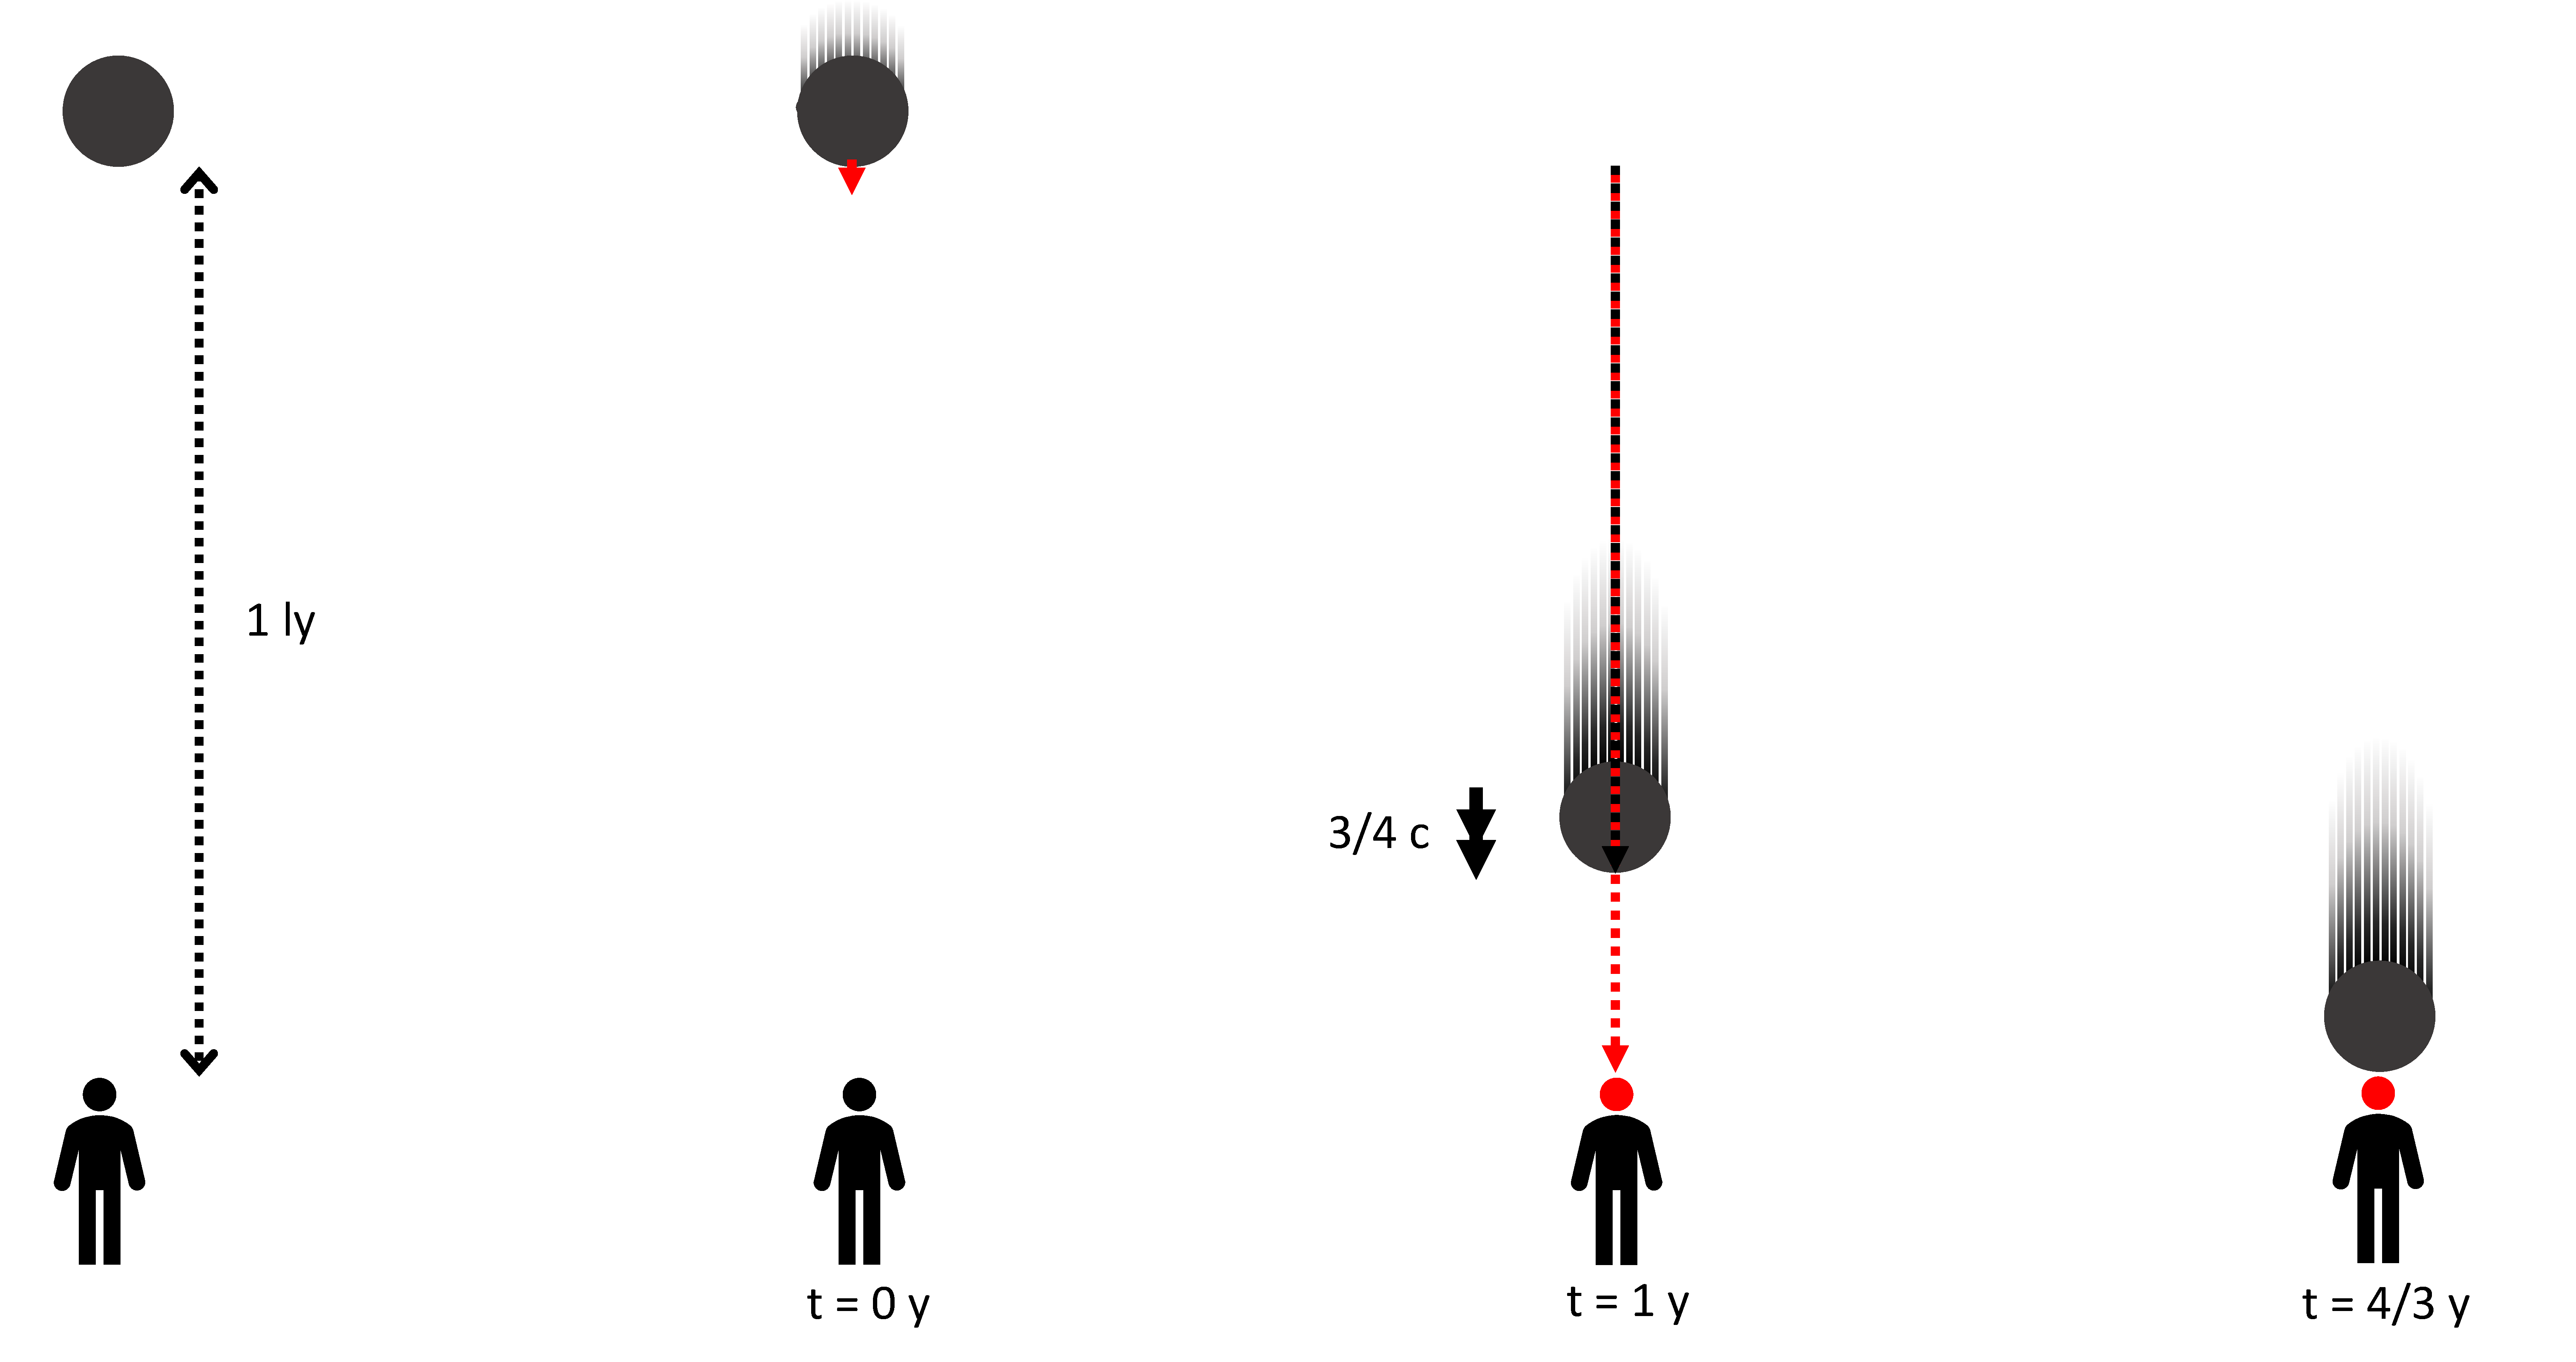
\includegraphics[width=10cm]{Perceived_speed.pdf}
    \caption{A diagram demonstrating the perceived speed of a ball vs its actual speed}
    \label{fig: perceived vs actual speed}
\end{figure}


%███████████████████████████████████████████████████████████████████
%███████████████████████████████████████████████████████████████████
\section{Velocity Transformation}

Previously, we explored how velocities at the speed of light change between different frames of reference, that is that their directions are aberrated, However, for objects moving at speeds less than light, we need the transforming speeds to be different as well as aberrated. As we need the \hyperlink{def-transform}{transform} to tend towards the classical \hyperlink{def-transform}{transform} as the speeds tend towards zero. To understand these velocity \hyperlink{def-transform}{transformation}s, we will need to first delve into the mathematical details which will be covered in later chapters.


%*** Javascript can redo lorry diagram but with speeds less than that of light, and have the time between emittion and absorbtion being same, but speeds and direction of pulse changing depending on rest direction

%*** javascript Diagram could have animated polar graph of how velocities change for low and fast velocities and frame changes *** could show classical addition of velocities in it too, either as an overlay, beside it or using button

% is there a way to visualise the change in none speed of light velocities


%███████████████████████████████████████████████████████████████████
%███████████████████████████████████████████████████████████████████
\section{The More Abstract Properties...}% of Momentum, Energy and Mass}

The \hyperlink{def-transform}{transformation} of more abstract quantities that depend on position and time, such as momentum, energy and mass do not have a simple visual interpretation, and this is the point at which the mathematics is needed for a proper understanding of how they transform. With the maths you will find new conservation of momentum and energy laws.

%*** could talk about what happens to the quantities without saying why

%This also means that it is impossible to get any particle with mass up to the speed of light, as the closer the particle gets to the speed of light, the heavier it is perceived and therefore keeps requiring a greater and greater force to accelerate it, This amount of perceived mass tends to infinity and the force required to accelerate it would also tend to infinity.\newline

%***
%(diagram)
%If we have two balls roll to the center of a truck at rest are and hit each other and stick, giving zero overall momentum as both balls momentum cancel out, but to observer on the road the stuck together balls move with the truck , so the ball at the back of the truck must have more momentum before the collision...
%*** so far this is also true for classical frame transform

%From before we have that the consequence of the different times and coordinates is that if a moving object emits light, to allow the speed of light to stay constant, the transform will also have the consequence of changing the frequency of the light, and hence its energy.

%Since energy is measured in units of position and time (as well as mass) the energy of a particle and systems in different frames have to go through transformations themselves, which leads to the famous energy and mass equivalence equation E=mc2 (this is the reduced form of equation)\newline

%From finding how the momentum changes between 2 frames due to the Lorentz transformations we find a relation between the Mass of a particle and how much energy that this particle is equivalent to, i.e. if a particle with a certain mass completely annihilates with its anti-particle, it gives out photons, corresponding to the energy of the particle which is different whether it is at rest or moving, as the perceived mass of a particle increases the faster it moves\newline

%*** mass is not increased only the apparent mass 


%This and the previous sections will also lead to changes in how we treat acceleration and forces, but these unfortunately have no simple visualisation for how they are transformed between frames.

%███████████████████████████████████████████████████████████████████
%███████████████████████████████████████████████████████████████████
\section{Summary}

A key early idea was that light travelled through a medium called the luminiferous aether. The Michelson-Morley experiment attempted to measure Earth's motion relative to this aether. Surprisingly, no difference was found in the speed of light regardless of direction. This conflicted with intuitive addition of velocities, discredited the aether theory, and led Einstein to propose light's constant speed in all frames as a fundamental principle. 

Special relativity emerged from the insight that light's speed in a vacuum is constant for all observers, regardless of the lights source's speed relative to each observer. This required rethinking the concepts of time intervals and distances between points to accommodate light's fixed speed and led to requiring that a clock moving relative to an observer ticks slower from the observer's perspective while also being contracted in the direction of its motion. This was shown in figure \ref{fig: truck clock} and figure \ref{fig: full truck transform}. 

It also led to the \hyperlink{def-simultaneity}{simultaneity} of events not being absolute, e.g. light emitted from the middle of a moving truck reaches the front and back walls at the same time to someone at rest in the truck. But someone standing still on the road sees the light hit both walls at different times, as shown in figure \ref{fig: truck simultaneity}. There is no universal "now" at a distance - observers relate events differently.

Classical physics provides an excellent approximation of reality at low speeds. Relativistic effects only become readily noticeable at speeds approaching light's. We don't normally experience them because motions in everyday life are very slow relative to light's which is roughly three hundred million metres per second. The faster an object moves relative to an observer, the more it's lengths contract and it's time dilates, to the observer.

When it comes to velocities, they combine differently than in classical physics. Though we must have that the transforms reduce to the intuitive addition of velocities of classical physics at low speeds while accommodating light's constant rate in all frames of reference. This leads to initially bizarre outcomes like \textbf{apparent} faster-than-light motion emerging from how relativistic optical effects play out across distances, due to the delay in light signals from objects at a distance. Nevertheless, special relativity gives a truer, more accurate picture of reality.

We also seen that lights frequencies shift when emitted from moving sources due to space-time effects on wave propagation, the Doppler effect, and that light concentrates in direction of source's motion, the aberrational effect. Both together intensely focus light and radiation in the direction of rapidly moving objects, relativistic beaming.

These effects will all be explained more fully with maths in the coming chapters, along with other effects that require the maths to fully understand, as well as new conservation laws of energy, mass and momentum. We will derive everything step by step starting with the transformation of positions and times between reference frames.


%* what will come later...



%███████████████████████████████████████████████████████████████████
%███████████████████████████████████████████████████████████████████
\section{Definitions}
%███
% need precisely one new line
%███

\section{Definitions}

\subsection{Mathematical Framework}%███

% {reference frame} {frame of reference}
\noindent \hypertarget{def-Reference-frame}{\textbf{Reference frame:}}
An abstract coordinate system that is taken to be at rest consisting of three spatial and one time axis. The origin, orientation, and scale of its axis are specified by a set of points in space. The purpose of it is to provide a standardized means of defining the position and orientation of objects at any instant in time.

% {Inertial reference frame} {Inertial frame of reference}
\noindent \hypertarget{def-Inertial-reference-frame}{\textbf{Inertial reference frame:}}
A reference frame that is not undergoing any acceleration. An observer's reference frame is inertial if they do not feel a force acting on them.

% {proper frame} {rest frame}
\noindent \hypertarget{def-proper-frame}{\textbf{Proper/Rest frame:}}
This is the reference frame of the observer or object itself.

%%% initial frame

% {Primed frame} {Prime frame}
\noindent \hypertarget{def-Primed-Frame}{\textbf{Primed frame:}}
A reference frame that is moving relative to the current frame.

% {frame velocity}
\noindent \hypertarget{def-frame-velocity}{\textbf{frame velocity:}}
The velocity of a reference frame relative to the current reference frame.

% {frame transform} {frame transformation} {transform} {transformation}
\noindent \hypertarget{def-transform}{\textbf{Frame transform:}}
The changing of coordinates and other quantities in a reference frame into their corresponding values in another reference frame.

% {galilean} {galilean transform} {classical transform} {Galilean frame transform} {classical frame transform} {classical tranformation}
\noindent \hypertarget{def-galilean-transform}{\textbf{Galilean/Classical frame transform:}}
Transformation of coordinates and physical quantities according to Newtonian physics between two frames of reference.

% {Relativistic transform} {Relativistic frame transform} {Relativistic tranformation} {lorentz transform} {lorentz transformation}
\noindent \hypertarget{def-lorentz-transform}{\textbf{Relativistic frame transform:}}
The changing of the spatial coordinates, the time coordinate, and other physical quantities into their corresponding values in a different inertial reference frame using equations from special relativity.

% {observer}
\noindent \hypertarget{def-observer}{\textbf{Observer:}}
An entity/thing with an associated frame of reference/system of coordinates, with respect to which you can measure objects' position, orientation, and other properties.

% {event}
\noindent \hypertarget{def-event}{\textbf{Event:}}
An occurrence that can be specified by a unique combination of the three spatial and one time coordinates. These four coordinates, together, form a point in spacetime.

% {simultaneous} {simultaneity} {simultaneously}
\noindent \hypertarget{def-simultaneity}{\textbf{Simultaneity:}}
Within a reference frame, two or more events are simultaneous if they occur at the same time within it. Classically, if any two events are simultaneous in one reference frame, they are also simultaneous in another. This is not true in special relativity, and the order of events can depend on the frame of reference.

% {retarded position}
\noindent \hypertarget{def-retarded-position}{\textbf{Retarded position:}}
The previous position of a field's source, that an observer sees it at, due to the time delay between when a moving source emits a field and when the observer detects that field.

\subsection{The Mechanics}%██████████████████

% {aether}
\noindent \hypertarget{def-aether}{\textbf{Aether:}}
A proposed medium that filled the vacuum of space that light propagated through.

% {vacuum}
\noindent \hypertarget{def-vacuum}{\textbf{Vacuum:}}
Empty space with no matter and negligible amount of effects from fields.

% {lorentz length contraction} {length contraction}
\noindent \hypertarget{def-length-contraction}{\textbf{Lorentz length contraction:}}
The shortening of an object along the direction of its motion relative to an observer (relative to the object at rest).

% {time dilation}
\noindent \hypertarget{def-time-dilation}{\textbf{Time dilation:}}
The slowing of the passing of time for objects in motion relative to an observer, compared to the passing of time for the observer.

% {doppler effect}
\noindent \hypertarget{def-doppler-effect}{\textbf{Doppler effect:}}
The change of a wave's frequency due to the motion of its source relative to an observer. This is due to the bunching up of the wave in the direction of movement of the source and the stretching of the wave in the opposite direction, as well as the dilation of time between two parts of the emitted wave.

% {aberration} {aberrated} {aberrate} {aberrating} {aberrates}
\noindent \hypertarget{def-aberration}{\textbf{Aberration of light:}}
The changing of the direction of the propagation of light when moving into another reference frame.

% {relativistic beaming} {beaming}
\noindent \hypertarget{def-relativistic-beaming}{\textbf{Relativistic beaming:}}
The accumulation of the Doppler effect and aberration of light, and how it affects the amount of light and its frequency emitted at different angles from a moving source. This effect can be extended to any wave or field emitted at the speed of light from a moving source.

% {retarded field}
\noindent \hypertarget{def-retarded-field}{\textbf{Retarded field:}}
A moving source's field, where at each point has been propagated at the speed of light from the retarded position of the source...

% {field}
\noindent \hypertarget{def-field}{\textbf{Field:}}
...

% {light year}
\noindent \hypertarget{def-light-year}{\textbf{Light year:}}
...

\subsection{Definitions for Later}%██████████████████

% {invariant} {lorentz invariant} {transform invariant}
\noindent \hypertarget{def-lorentz-invariant}{\textbf{Transform Invariant:}}
...

% {postulate} {postulates}
\noindent \hypertarget{def-postulates}{\textbf{Postulates:}}
...

% {flux}
\noindent \hypertarget{def-flux}{\textbf{Flux:}}
describes the rate at which a quantity flows across a surface (flowrate per unit area)

%███████████████████████████████████████████████████████████████████
%███████████████████████████████████████████████████████████████████
%███████████████████████████████████████████████████████████████████
\chapter{Positions and Time} %The Math Begins: 

**** could include graphs of classical vs relativistic quantities in swapping frames, either both quantities or graph of ratios, throughout sections

Now that we have learned about the basic concepts of special relativity, we can let the mathematics begin, starting with classical relativity as a starting point, it will give us an understanding of how to \hyperlink{def-transform}{transform} between \hyperlink{def-Reference-frame}{reference frame}s, we can then compare special relativity to this to help with our intuition.


%███████████████████████████████████████████████████████████████████
%███████████████████████████████████████████████████████████████████
\section{Classical Relativity}%%%%%%%%%%%%%

For classical (Galilean) relativity, if we have two \hyperlink{def-observer}{observer}s moving relative to each other at constant velocity and want to find how each \hyperlink{def-observer}{observer} would describe the positions and motion of a particle relative to them, we need to know the positions and times in one observer's frame and how to \hyperlink{def-transform}{transform} them into the other \hyperlink{def-observer}{observer}s frame. i.e. if we have how one \hyperlink{def-observer}{observer} would describe the coordinates of a particle over time relative to them and we want to now know the coordinates of the particle with respect to the other \hyperlink{def-observer}{observer}, we need to know how the transformation of coordinates works.

Before special relativity it was assumed that distances between two positions was the same for all \hyperlink{def-observer}{observer}s, i.e. the first \hyperlink{def-observer}{observer} would see a stick and measure it to be the same length as another \hyperlink{def-observer}{observer} moving relative to them would measure it to be. long story short, lengths are the same for all \hyperlink{def-observer}{observer}s in \hyperlink{def-galilean-transform}{Galilean transform}. Another assumption is that time is constant for everyone, i.e. clocks move at same rate for each \hyperlink{def-observer}{observer} and if a particle was to emit light at a particular time. This light would be emitted at the same time for the other \hyperlink{def-observer}{observer}s too.

So lets see how the mathematics works for the classical coordinate system transform between two \hyperlink{def-observer}{observer}s. If we have the coordinate system in one \hyperlink{def-Inertial-reference-frame}{inertial reference frame} $<S>$ to describe an \hyperlink{def-event}{event} $E$, which is given by the set of spatial and time coordinates $(x,y,z)$ and $t$, and we want to find the coordinates of the event in another "primed" \hyperlink{def-Inertial-reference-frame}{inertial reference frame}/coordinate system that is moving at a relative speed $v$ to the first frame in the z-axis, that was initially overlapping with the first frame at time $t=0$, with the events coordinates now described by $x',y',z'$ at time $t'$. The direction of second frame is in the upwards z-direction instead of being to the right in the case of the truck diagrams from the previous chapter, this to help us when we use spherical polar coordinates later and to help see the symmetries.

\begin{figure}[H]
\centering
\tikzsetnextfilename{Tikz_simple_Galilean_transform_derivation}
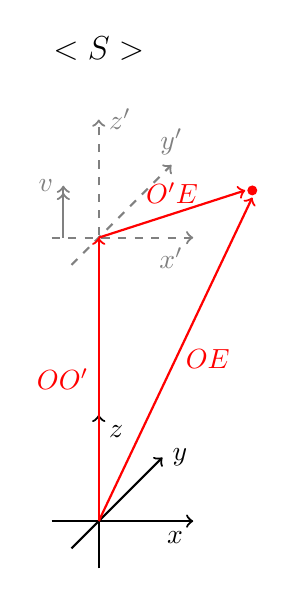
\begin{tikzpicture}[scale=3]%,tdplot_main_coords]
\coordinate (O) at (0,0,0);
%
\draw (1.7,2,0) node{ {\large $<S>$}};
\draw[black, thick,->] (1.5,0,0) -- (2.1,0,0) node[anchor=north east]{$x$};
\draw[black, thick,->] (1.7,-0.2,0) -- (1.7,0.45,0) node[anchor=north west]{$z$};
\draw[black, thick,->] (1.7,0,0.3) -- (1.7,0,-0.7) node[anchor=west]{$y$}; 
%
\draw[gray, dashed, thick,->] (1.5,1.2,0) -- (2.1,1.2,0) node[anchor=north east]{$x'$};
\draw[gray, dashed, thick,->] (1.7,1,0) -- (1.7,1.7,0) node[anchor= west]{$z'$};
\draw[gray, dashed, thick,->] (1.7,1.2,0.3) -- (1.7,1.2,-0.8) node[anchor=south]{$y'$}; 
\draw[gray, thick, ->>] (1.55,1.2,0) -- (1.55,1.42,0) node[anchor=east]{$v$};
\fill[red] (2.35,1.4,0) circle (0.6pt);
%
\draw[red, thick, ->] (1.7,0,0) -- (2.35,1.37,0) node[midway,anchor=west]{$OE$};
\draw[red, thick, ->] (1.7,0,0) -- (1.7,1.2,0) node[midway,anchor=east]{$OO'$};
\draw[red, thick, ->] (1.7,1.2,0) -- (2.32,1.4,0) node[midway,anchor=south]{$O'E$};
%
\end{tikzpicture}
\caption{Diagram, of a \protect\hyperlink{def-Reference-frame}{reference frame} $<S>$ with its associated $(x,y,z)$ coordinate system at rest in this frame, it also shows a primed coordinate axis $(x',y',z')$ at time $t=t'$ from when the axis where overlapping, associated with another \protect\hyperlink{def-Inertial-reference-frame}{inertial reference frame}s moving at velocity $v$ in the z-axis, it shows an \protect\hyperlink{def-event}{event} with position vector $\overrightarrow{OE}$ in this frame and the vector $\overrightarrow{OO'}$ to this primed axis origin and the vector $\overrightarrow{O'E}$ which is vector from this primed origin to the \protect\hyperlink{def-event}{event} in the shown frame.}
\label{simple Galilean transform derivation}
\end{figure}


For frame $<S>$ we have it's origin $O$ and an \hyperlink{def-event}{event} $E$ located at
\begin{equation}%%%%%%%%%%%%%%%
    \overrightarrow{OE}=(x,y,z)
\end{equation}%%%%
at time $t$ from axis overlap, and a prime frame $<S'>$'s origin $O'$ moving at relative velocity $v$, so that in the original frame we have after a time 
\begin{equation}%%%%%%%%%%%%%%%
    \overrightarrow{OO'}=(0,0,vt)
\end{equation}%%%%
in $<S'>$ we have the \hyperlink{def-event}{event}'s coordinates as 
\begin{equation}%%%%%%%%%%%%%%%
    \overrightarrow{O'E} = (x',y',z') = \overrightarrow{OE} - \overrightarrow{OO'}  = (x,y,z-vt)
\label{eq: classical event}
\end{equation}%%%%

for frame $<S>$ we have 
\begin{equation}%%%%%%%%%%%%%%%
    \overrightarrow{OE} = (x,y,z) = \overrightarrow{OO'} + \overrightarrow{O'E} = (x',y',z'+vt')
\label{eq: classical event 2}
\end{equation}%%%%

so we have $x=x'$, $y=y'$, $t=t'$ (time is assumed to be the same across reference frames in classical relativity) and for the z-components
\begin{equation}%%%%%%%%%%%%%%%
    \begin{aligned}
      &  z' = z - vt \\
       & z = z'+vt'
    \end{aligned}
\end{equation}%%%%
This shows the symmetry between the frames, as if we where originally in the $<S'>$ frame we would have the $<S>$ frame moving at -$v$ relative to it, so we would expect that the inverse \hyperlink{def-transform}{transformation} would replace one frames coordinates with the other and have the the opposite \hyperlink{def-frame-velocity}{frame velocity} instead.
So the inverse of going from \hyperlink{def-Primed-Frame}{primed frame} to original is just a matter of swapping all primed coordinates with original coordinates and changing the sign on the \hyperlink{def-frame-velocity}{frame velocity}, this can be seen from starting at time $t=0$ we have the frames origins overlapping and that there is a symmetry from here, we have the freedom to choose either frame to be the original, as no frame is particularly special and depending which one you pick the relative velocity is either $v$ or -$v$.

The full description of the position and time \hyperlink{def-transform}{transform} for an \hyperlink{def-event}{event} is given as

\begin{equation}%%%%%%%%%%%%%%%
    \begin{aligned}
      &  x'=x \\ & y'=y \\ &z' = z-vt  \\ 
      \text{at time \ \ \ } \\
      & t'= t  
    \end{aligned}
    \label{eq: Galilean transformation}
\end{equation}%%%%


%███████████████████████████████████████████████████████████████████
%███████████████████████████████████████████████████████████████████
\section{Postulates of Special Relativity}%%%%%%%%%%%%%
 
\begin{tcolorbox}[breakable]
\begin{enumerate}
    \item The laws of physics are the same in all \hyperlink{def-Inertial-reference-frame}{inertial frames of reference} (i.e. if an \hyperlink{def-observer}{observer} carries out an experiment in an \hyperlink{def-Inertial-reference-frame}{inertial reference frame}, there would be no difference if the experiment was instead carried out within a different \hyperlink{def-Inertial-reference-frame}{inertial reference frame})
    \item The speed of light in a \hyperlink{def-vacuum}{vacuum} is the same in all inertial/non-accelerating frames of reference.
\end{enumerate}
\end{tcolorbox}

They are not the only assumptions, you may notice some small jumps in the logic when it comes to the derivation. But be aware small miss understandings have thrown people down the special relativity rabbit hole when trying to find inconsistencies or prove it wrong, through out this I will try to leave as few logical gaps as possible, and explain as simply and as in depth as possible so that you do not do this yourself.

%███████████████████████████████████████████████████████████████████
%███████████████████████████████████████████████████████████████████
\section{Derivations}% from Time Dilation and Length Contraction}
We will be following a similar thought pattern as in the conceptual introduction for the derivations, an alternative derivation using spherical light pulses is given in Appendix \ref{spherical light pulse derivation}.

%███████████████████████████████████████████████████████████████████
\subsection{Time Dilation}

\begin{figure}[ht]
\centering
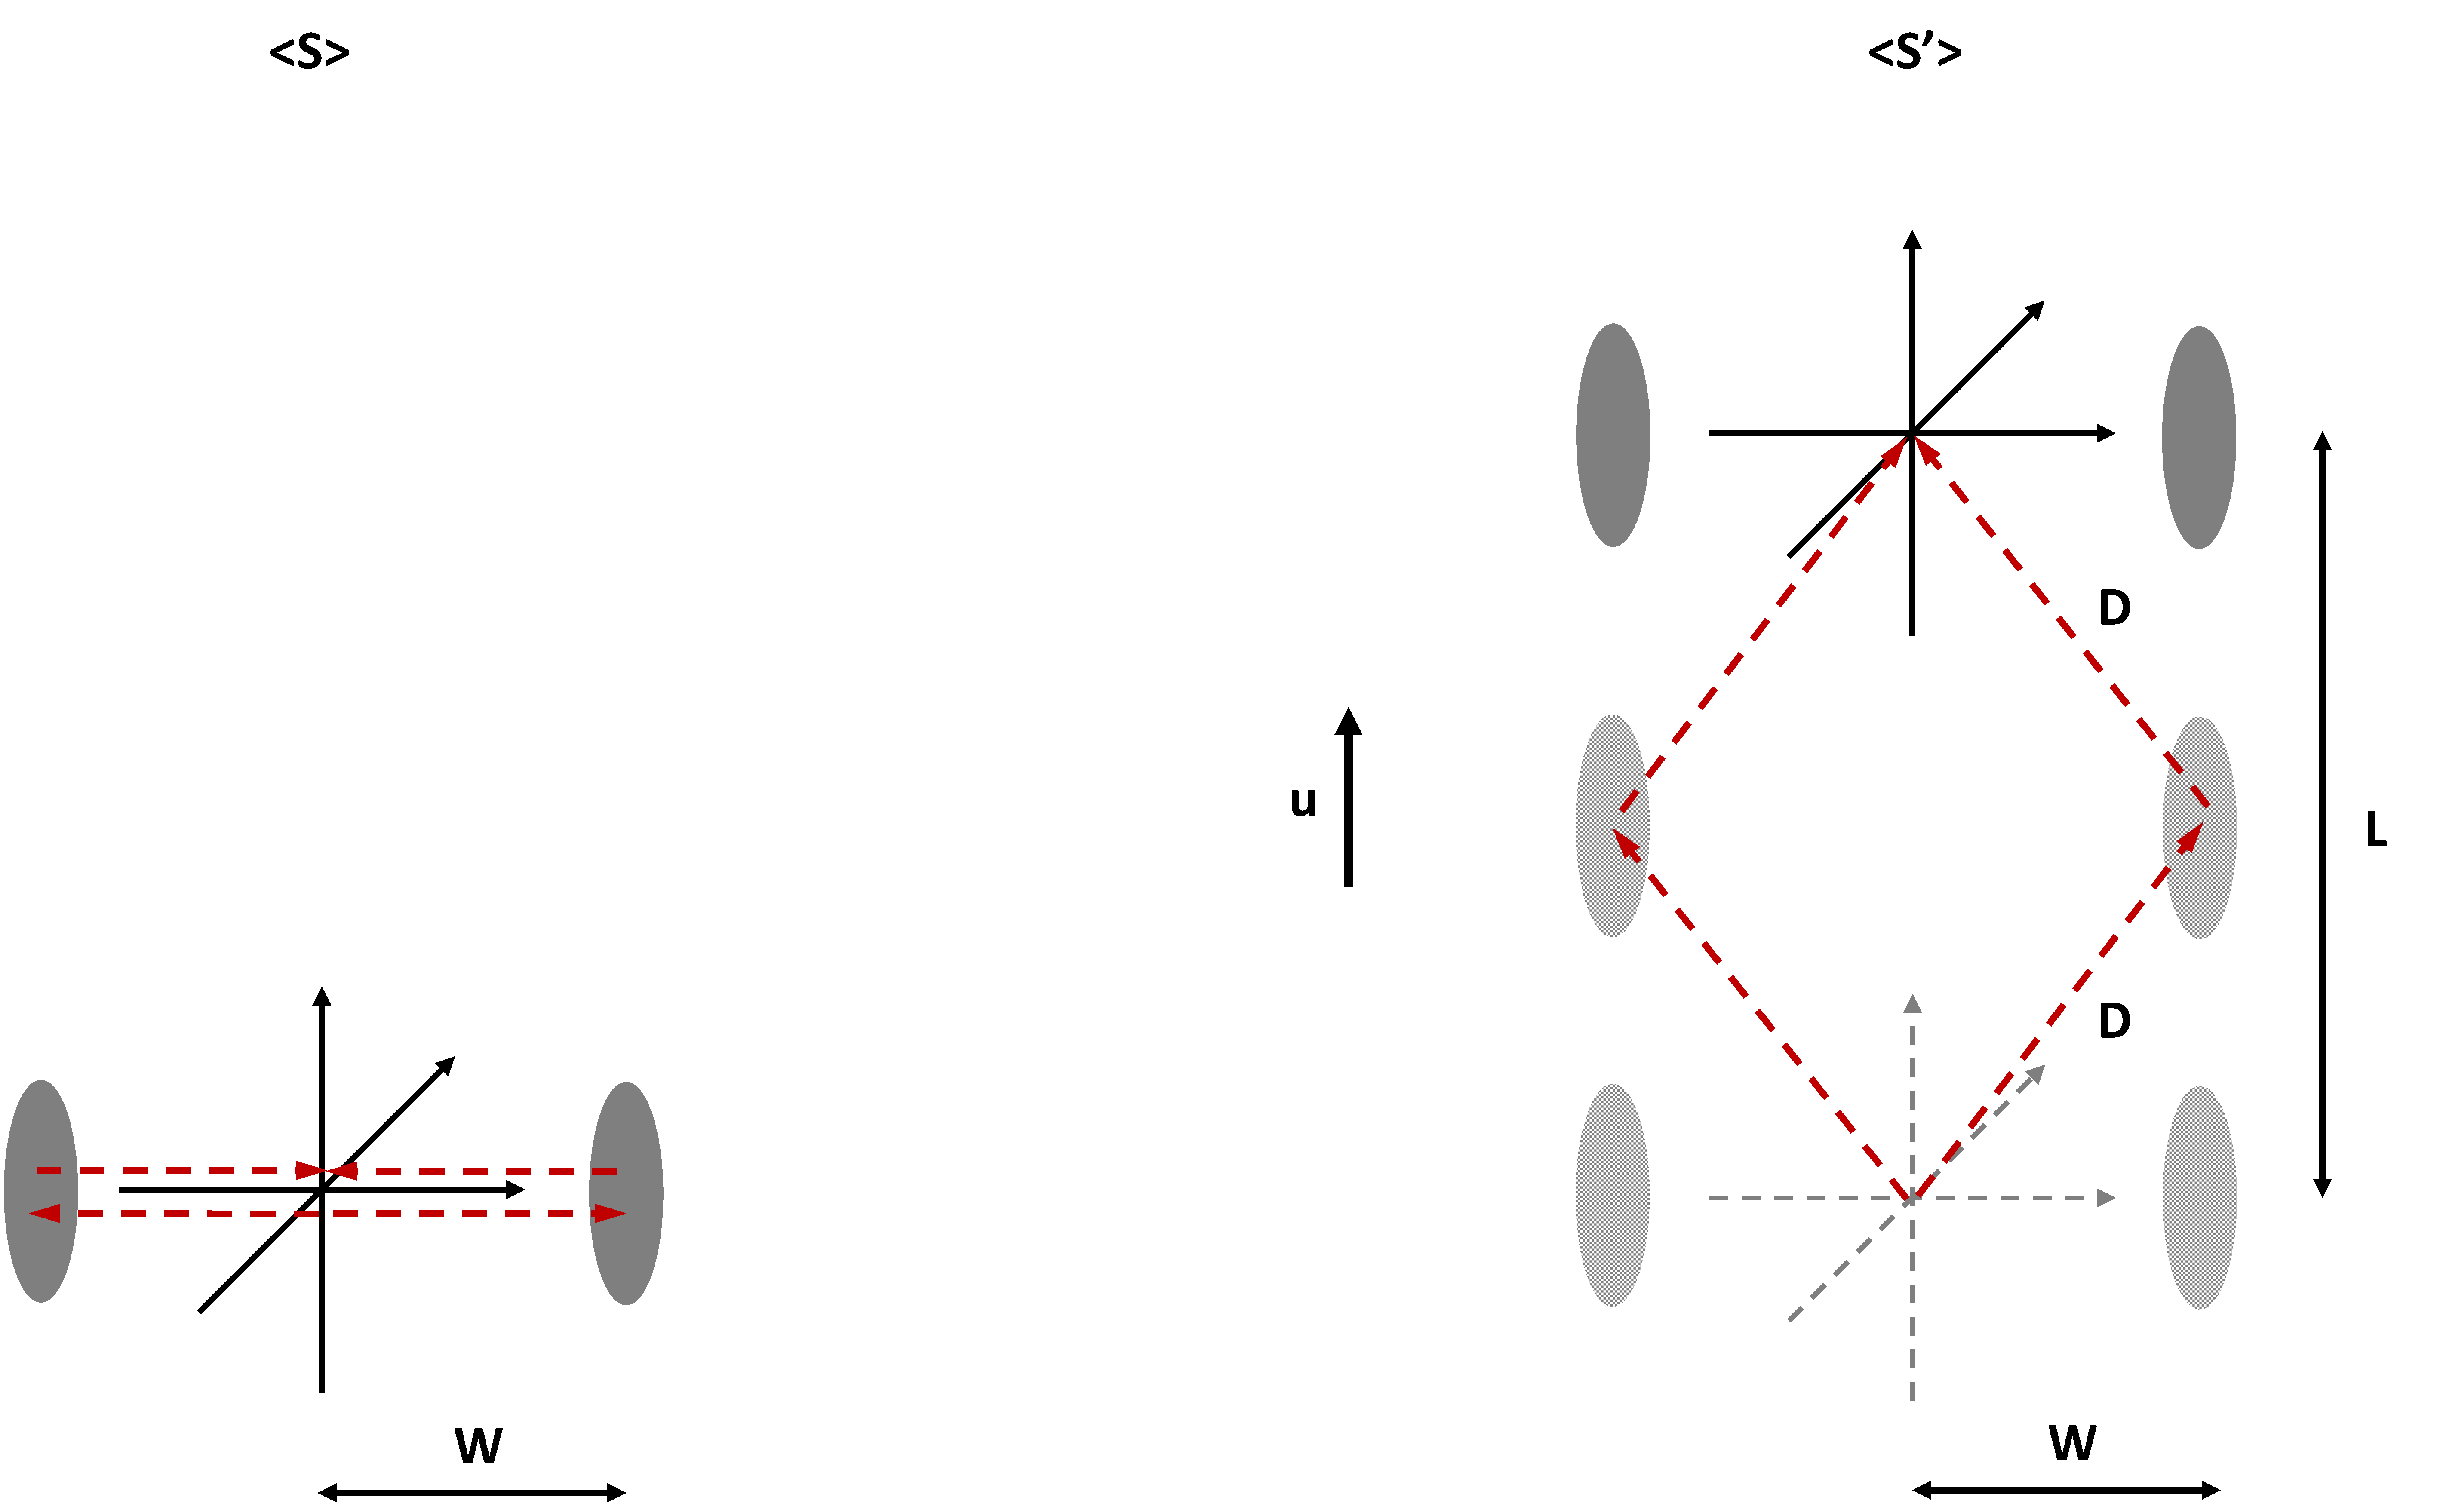
\includegraphics[width=10cm]{Light_clock.pdf}
    \caption{A diagram showing a clock keeping time using light, light is emitted from the origin and reflected off a mirror back to the origin, shown here in two different frames (describe what things are in diagram)(need axis labels)}
    \label{fig: light clock}
\end{figure}

We can have a clock which keeps time using a light pulse being emitted from a bulb towards a mirror and back again, recording a tick on its clock each time it returns to were it was emitted, taking a time $\Delta \tau$ in the rest frame to return. The distance the light travels to the mirror and back in this time is
\begin{equation}
    2W=c\Delta \tau,
\end{equation}
the distance the bulb travels during this in the moving frame is 
\begin{equation}
    L=u\Delta t' = -v \Delta t',
\end{equation}
where $\Delta t'$ is the time it took light to return in moving frame and $u$ is the speed of the bulb which is in the opposite direction of the \hyperlink{def-Primed-Frame}{primed frame} relative to the \hyperlink{def-proper-frame}{proper frame}, i.e. $u=-v$, the distance light travels in this time is 
\begin{equation}
    2D=c\Delta t',
\end{equation} 
this forms a triangle, so we have the square of the hypotenuse $2D$ equal to the square of the lengths $W$ and $L$:
\begin{equation}%%%%%%%%%%%%%%%
    c^2 \Delta t'^2 = v^2 \Delta t'^2 + c^2\Delta \tau^2 
\end{equation}%%%%
rearranging to find the time it took in the \hyperlink{def-Primed-Frame}{primed frame} relative to the time in the \hyperlink{def-proper-frame}{proper frame}, we find 
\begin{equation}%%%%%%%%%%%%%%%
     \Delta t' = \dfrac{1}{\sqrt{1-\dfrac{v^2}{c^2}}} \Delta \tau = \gamma \Delta \tau
\end{equation}%%%%
with 
\begin{equation}%%%%%%%%%%%%%%%
   \gamma =  \dfrac{1}{\sqrt{1-\dfrac{v^2}{c^2}}}.
\end{equation}%%%%

The Time taken between two \hyperlink{def-event}{event}s in the same position in the moving frame takes longer than in the \hyperlink{def-proper-frame}{rest frame} of the clock, due to the longer distance it has to travel at the same speed.

%███████████████████████████████████████████████████████████████████
\subsection{Length Contraction TODO}

\begin{figure}[H]
\centering
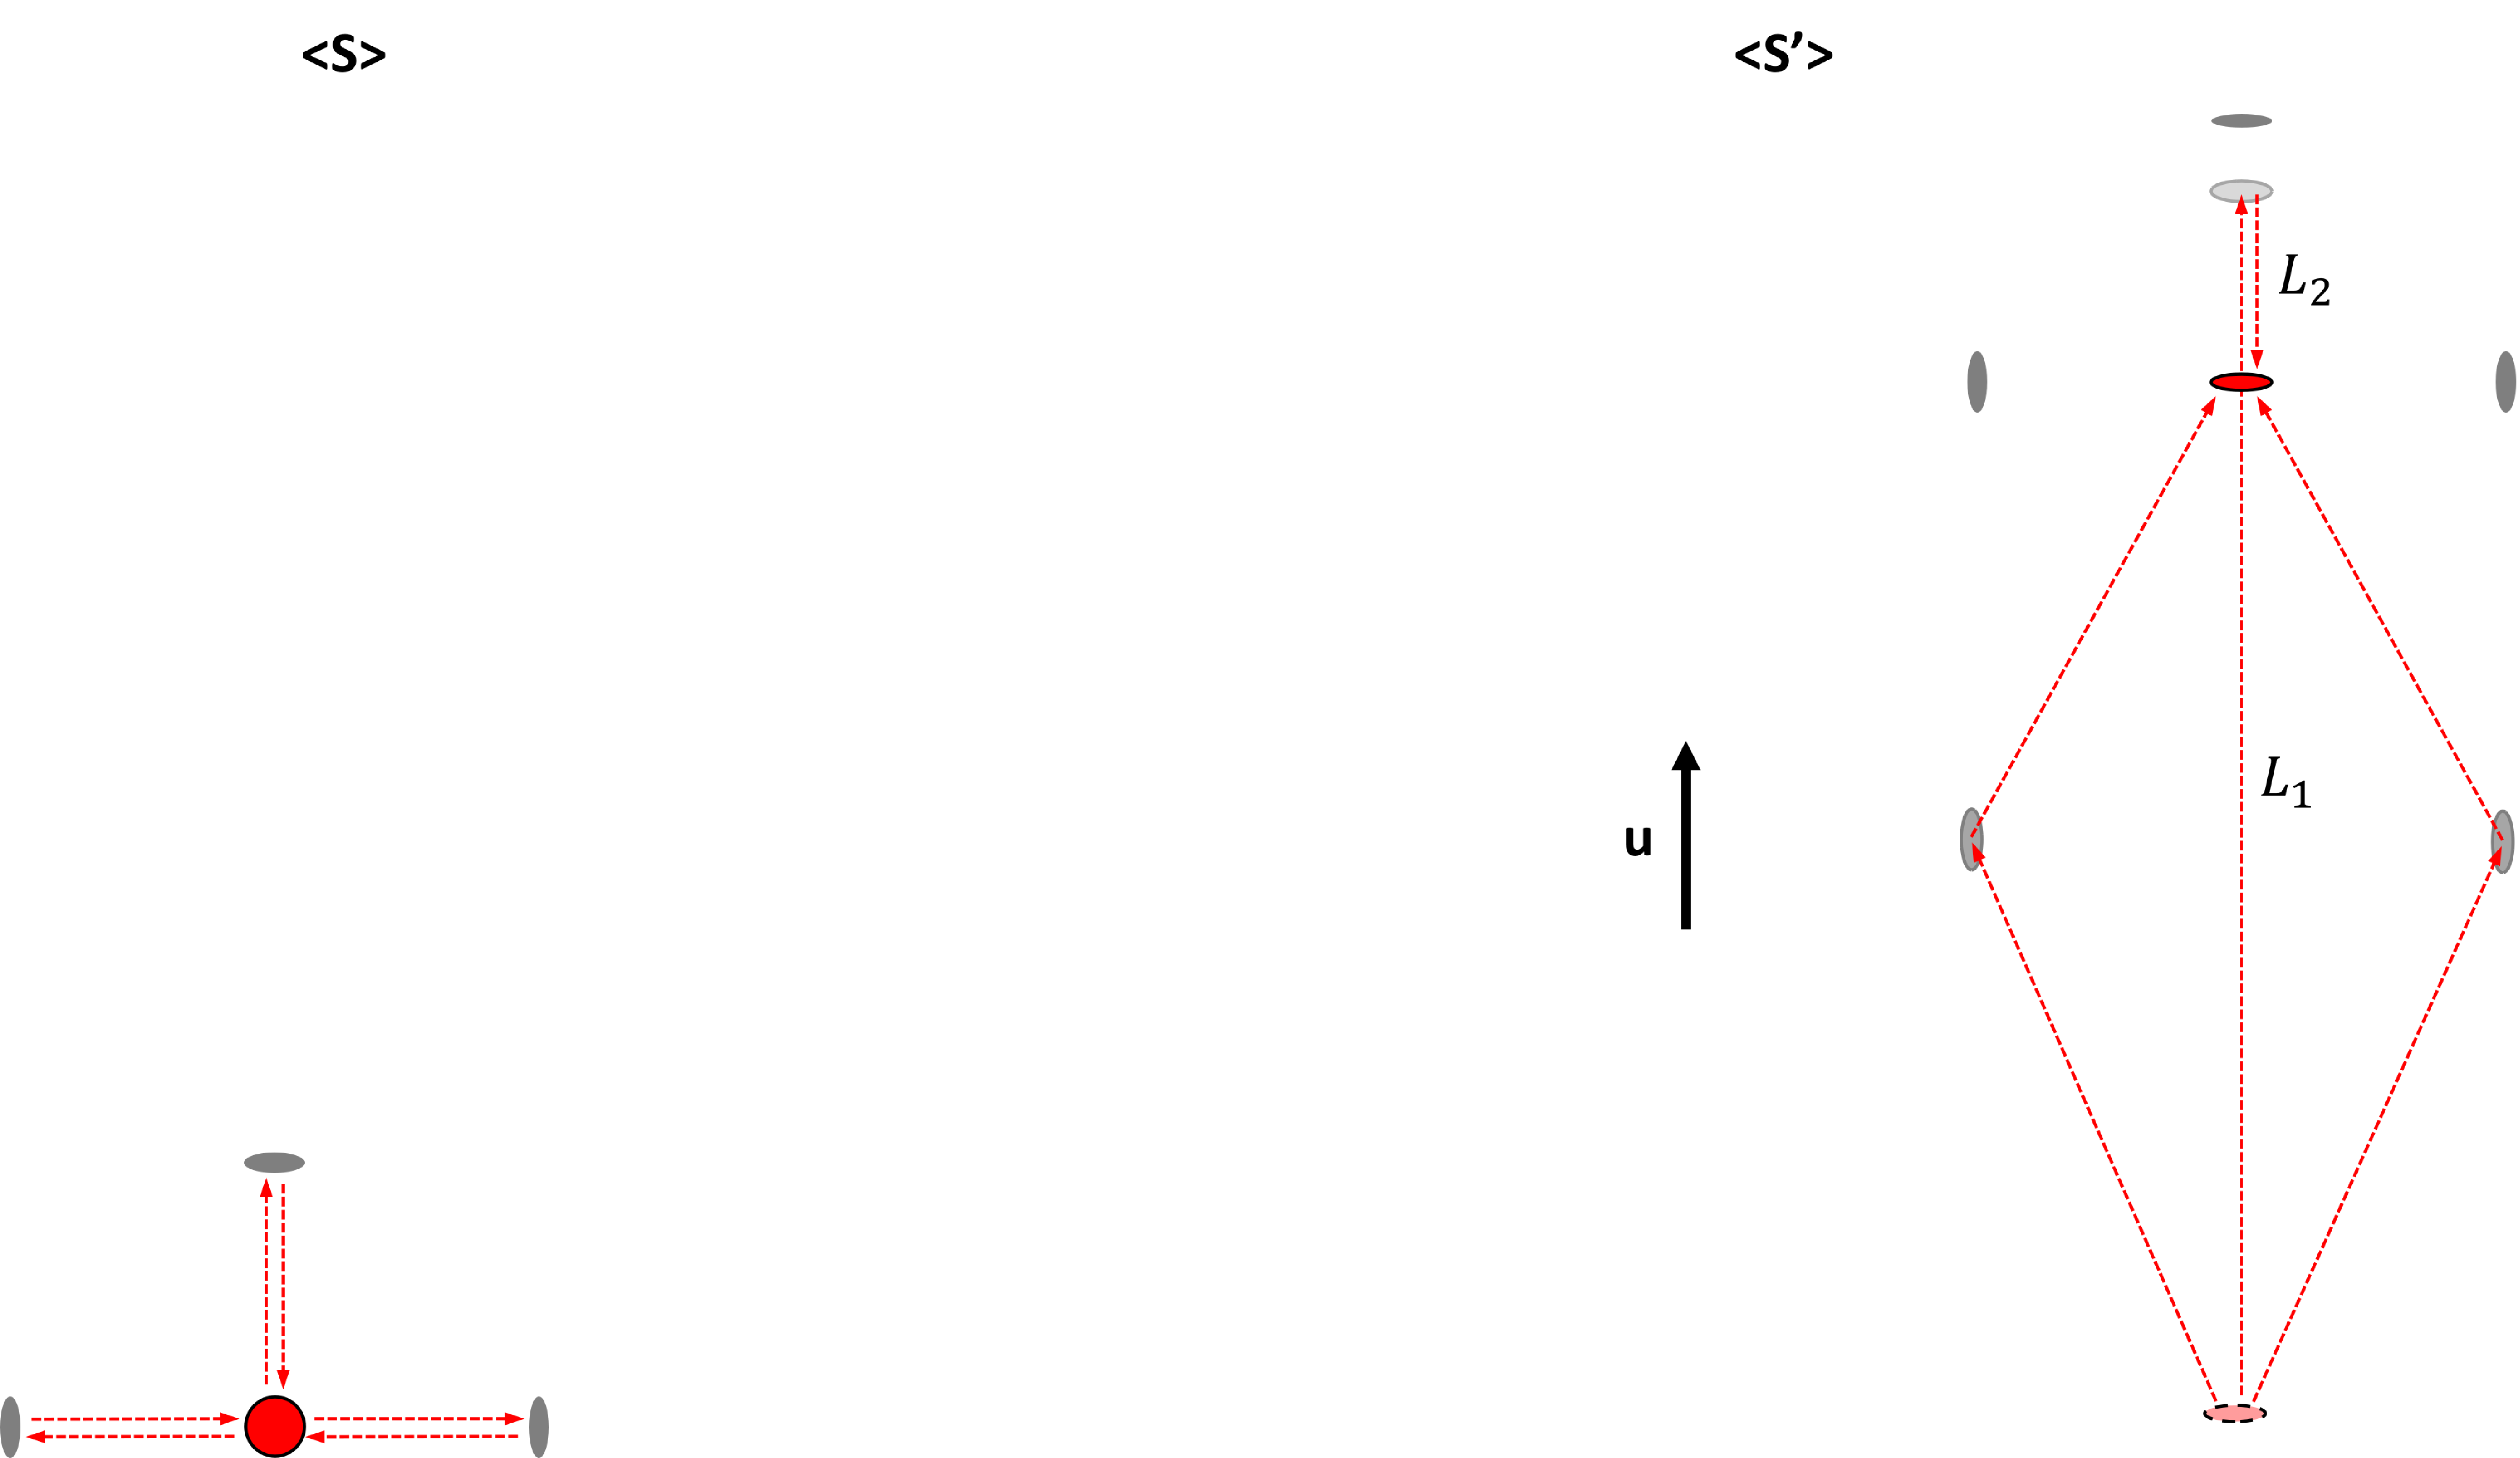
\includegraphics[width=10cm]{Length_Contraction.pdf}
    \caption{A diagram, showing a central bulb emitting light in the four directions, with all light being reflected by the mirrors back to the centre, this is shown at rest on the left and moving in another inertial frame with the system now moving, with its length slightly contracted in the direction of movement.}
    \label{fig: length contraction math}
\end{figure}

If we have a system in its rest frame with light emitted in all four directions from the centre, so that it will bounce off the mirrors return to the centre simultaneously. we require that in the moving frame they also all return to the centre simultaneously, as multiple events that happen at a single point simultaneously in one frame, must happen simultaneously in all other frames. This time between light being emitted and absorbed will be the dilated time from previous section. To achieve this simultaneity in the return of the light to the bulb, the length of the full path of light from there centre to the mirrors and back in each direction has to be the same (as its speed of light is same in all directions and the return time has to be the same), we can work out the length of the sideways paths from the time dilation section, and this is the length the path needs to be in the vertical directions as well, the paths can only have this length if the system length is contracted when moving in the direction of movement. Noting that there is no contraction in the perpendicular diction to the movement due to the paradox explained in chapter \ref{width contraction}.

*the pulse sent backwards has distance 
\begin{equation}
    L_1= ct'_1= D' - ut'_1
\end{equation} 
to travel to back mirror that is moving towards the point it was emitted, and then has to travel back to the bulb a distance 
\begin{equation}
    L_2 = ct'_2= D' + ut'_2
\end{equation} 
giving 
\begin{equation}
    t'_1=\frac{D'}{c+u}
\end{equation}
and 
\begin{equation}
    t'_2=\frac{D'}{c-u}
\end{equation}
adding both times together gives total primed time 
\begin{equation}
    t' = D'(\frac{1}{c-u} + \frac{1}{c+u})=...=\frac{D'}{c}\frac{1}{1-u^2/c^2} =\frac{D'}{c}\frac{1}{1-v^2/c^2}=\gamma^2 \frac{D'}{c}
\end{equation}
giving 
\begin{equation}
    ct'=c\gamma t = \gamma D = \gamma^2 D'
\end{equation}
and finally leading to 
\begin{equation}
    D' = \frac{1}{\gamma}D
\end{equation}


%███████████████████████████████████████████████████████████████████
\subsection{Position and Time Transformation}

\begin{figure}[H]
\centering
\tikzsetnextfilename{Tikz_simple_lorentz_transform_derivation}
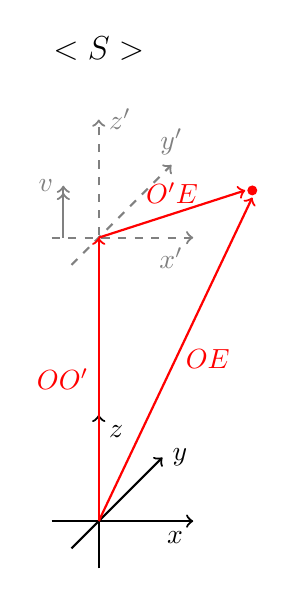
\begin{tikzpicture}[scale=3]%,tdplot_main_coords]
\coordinate (O) at (0,0,0);
%
\draw (1.7,2,0) node{ {\large $<S>$}};
\draw[black, thick,->] (1.5,0,0) -- (2.1,0,0) node[anchor=north east]{$x$};
\draw[black, thick,->] (1.7,-0.2,0) -- (1.7,0.45,0) node[anchor=north west]{$z$};
\draw[black, thick,->] (1.7,0,0.3) -- (1.7,0,-0.7) node[anchor=west]{$y$}; 
%
\draw[gray, dashed, thick,->] (1.5,1.2,0) -- (2.1,1.2,0) node[anchor=north east]{$x'$};
\draw[gray, dashed, thick,->] (1.7,1,0) -- (1.7,1.7,0) node[anchor= west]{$z'$};
\draw[gray, dashed, thick,->] (1.7,1.2,0.3) -- (1.7,1.2,-0.8) node[anchor=south]{$y'$}; 
\draw[gray, thick, ->>] (1.55,1.2,0) -- (1.55,1.42,0) node[anchor=east]{$v$};
\fill[red] (2.35,1.4,0) circle (0.6pt);
%
\draw[red, thick, ->] (1.7,0,0) -- (2.35,1.37,0) node[midway,anchor=west]{$OE$};
\draw[red, thick, ->] (1.7,0,0) -- (1.7,1.2,0) node[midway,anchor=east]{$OO'$};
\draw[red, thick, ->] (1.7,1.2,0) -- (2.32,1.4,0) node[midway,anchor=south]{$O'E$};
%
\end{tikzpicture}
\caption{one frame of \protect\hyperlink{def-event}{event}...}
\label{simple lorentz transform derivation}
\end{figure}

For frame $<S>$ we have it's origin $O$ and an \hyperlink{def-event}{event} $E$ located at $\overrightarrow{OE}=(x,y,z)$ and a prime frame's $<S'>$ origin $O'$ moving at relative velocity $v$, so that in the original frame we have after a time $t$, $\overrightarrow{OO'}=(0,0,vt)$. now from the last section, we have $z'$ for the z-component of $\overrightarrow{O'E}$ in the \hyperlink{def-Primed-Frame}{primed frame}, length contracted in this frame as $z'/\gamma$ so that $\overrightarrow{O'E} = (x,y,z'/\gamma)$ with the x and the y-components unaffected due to the cannon and ball thought experiment.
so that we have in frame $<S>$
\begin{equation}%%%%%%%%%%%%%%%
    \overrightarrow{OE}= \overrightarrow{OO'} + \overrightarrow{O'E}
\label{eq: event}
\end{equation}%%%%
subbing in each part into this equation and rearranging the z-component we have 
\begin{equation}%%%%%%%%%%%%%%%
    z' = \gamma (z-vt)
\end{equation}%%%%
now in frame $<S'>$ we have $\overrightarrow{OE}=(x,y,z/\gamma)$, $\overrightarrow{OO'}=(0,0,vt')$, $\overrightarrow{O'E} = (x,y,z')$, doing the same for these we have 
\begin{equation}%%%%%%%%%%%%%%%
    z = \gamma (z'+vt')
\end{equation}%%%%
Which should be expected as this shows the expected symmetry between the frames, as if we where originally in the $<S'>$ frame we would have the $<S>$ frame moving at -$v$ relative to the $<S'>$ frame, so we would expect that the inverse \hyperlink{def-transform}{transformation} would replace one frames coordinates with the other and have the the negative of the velocity instead.
Now substituting these into eachother we have
\begin{equation}%%%%%%%%%%%%%%%
    z = \gamma ( \gamma (z-vt)+vt')
\end{equation}%%%%
and rearranging gives
\begin{equation}%%%%%%%%%%%%%%%
    t' = \gamma \left( \left( \dfrac{1}{\gamma^2}-1 \right)\frac{z}{v} + t \right)
\end{equation}%%%%
with $\gamma^{-2}=1-v^2/c^2$ then giving
\begin{equation}%%%%%%%%%%%%%%%
    t' = \gamma \left( t - \dfrac{vz}{c^2} \right)
\end{equation}%%%%
leaving full description of the location and time of an \hyperlink{def-event}{event} as
\begin{equation}%%%%%%%%%%%%%%%
\mhl{
    \begin{aligned}
      &  x'=x \\ & y'=y \\ &z' = \gamma (z-vt)  \\ 
      \text{at time \ \ \ } \\
      & t'=\gamma \bigg(t-\frac{vz}{c^2}\bigg)  \\
      \text{with \ \ \ } \\
      &  \gamma = \dfrac{1}{\sqrt{1-\frac{v^2}{c^2}}}
    \end{aligned}
    } 
    \label{eq: Lorentz transformation}
\end{equation}%%%%

for the time \hyperlink{def-transform}{transform} the $\frac{vz}{c^2}$ term is the cause of the \hyperlink{def-event}{event}s no longer being \hyperlink{def-simultaneity}{simultaneous} in another inertial frame, and the gamma factor $\gamma$, is the the term that causes the overall change in how fast time flows relative in each frame.


%███████████████████████████████████████████████████████████████████
\subsection{Transforms with Low Relative Frame Speed Change}
*** classical \hyperlink{def-galilean-transform}{Galilean coordinates transform} obtained for small velocities, i.e. $v\ll c$ we have $\gamma \approx 1$ and
\begin{equation}%%%%%%%%%%%%%%%
    t' \approx t
\end{equation}%%%%
\begin{equation}%%%%%%%%%%%%%%% 
    z' \approx z - vt
\end{equation}%%%%
which is the expected result for the \hyperlink{def-galilean-transform}{Galilean coordinates transform} , and what way we expect things to work in everyday life. 

%███████████████████████████████████████████████████████████████████
%███████████████████████████████████████████████████████████████████
\section{Variables}
\section{Variables}

\noindent ${E}$ \textbf{:}
an \hyperlink{def-event}{event} given by the set of spatial and time coordinates. %*** might be confused with energy later ***

\noindent ${O},{O'}$ \textbf{:}
Position of proper and primed axis' origin, given by the set of spatial and time coordinates.

\noindent ${v}$ \textbf{:}
is the velocity of second \hyperlink{def-Reference-frame}{reference frame} relative to the first \hyperlink{def-Reference-frame}{reference frame}

\noindent ${c}$ \textbf{:}
the speed that light travels in empty space when it is not impeded by matter and fields.

\noindent ${\vec{r}}=({x},{y},{z},{t})$ \textbf{:}
are the position and time coordinates of \hyperlink{def-event}{event} in current \hyperlink{def-Inertial-reference-frame}{inertial reference frame}

\noindent ${\vec{r}'}=({x'},{y'},{z'},{t'})$ \textbf{:}
are the corresponding position and time coordinates the \hyperlink{def-event}{event} in another \hyperlink{def-Inertial-reference-frame}{inertial reference frame}, referred to as the \hyperlink{def-Primed-Frame}{primed frame}, and denoted with a ${'}$.

\noindent ${\gamma}$ \textbf{:}
a relativistic factor given by ${1/\sqrt{1-v^2/c^2}}$ which determines how much of an effect the \hyperlink{def-transform}{transform} of the coordinates deviates from the classical transform. It is only significant at relative frame speeds close to that of light.

\noindent ${\tau}$ \textbf{:}
the time of an \hyperlink{def-event}{event} in the \hyperlink{def-proper-frame}{rest frame} of an \hyperlink{def-observer}{observer}.

\noindent ${\Delta \tau,\Delta \tau'}$ \textbf{:}
...

\noindent ${\Delta x},{\Delta y},{\Delta z},{\Delta t}$ \textbf{:}
...

\noindent ${\Delta x'},{\Delta y'},{\Delta z'},{\Delta t'}$ \textbf{:}
...

\noindent ${dx},{dy},{dz},{dt}$ \textbf{:}
...

\noindent ${\vec{U}}=({u_x},{u_y},{u_z})$ \textbf{:}
...

\noindent ${\vec{U}'}=({u'_x},{u'_y},{u'_z})$ \textbf{:}
...

\noindent ${d\vec{U}},{d\vec{U}'}$ \textbf{:}
...

\noindent ${\vec{a}},{\vec{a}'}$ \textbf{:}
...



%███████████████████████████████████████████████████████████████████
%███████████████████████████████████████████████████████████████████
%███████████████████████████████████████████████████████████████████
\chapter{Velocity and Acceleration}
*** diagram *** \newline
The change in position of particle $\Delta \mathbf{R}_p$, with initial position $\mathbf{R}_0$, and a constant velocity 
\begin{equation}%%%%%%%%%%%%%%%
    \mathbf{U}_p = \begin{pmatrix}
    u_x \\ u_y \\ u_z \\
    \end{pmatrix}
\end{equation}%%%%
between time $t_1$ and $t_2$ is
\begin{equation}%%%%%%%%%%%%%%%
    \Delta \mathbf{R}_p = (\mathbf{R}_0 +\mathbf{U}_p t_2) - (\mathbf{R}_0 +\mathbf{U}_p t_1) =  (t_2 - t_1) \mathbf{U}_p =  \mathbf{U}_p \Delta t 
\end{equation}%%%%
(acceleration as well, but these will become negligible when we take an infinitesimal time interval later)
The \hyperlink{def-lorentz-transform}{Lorentz transformation} for this with $t=0$ is 
\begin{equation}%%%%%%%%%%%%%%%
    \Delta \mathbf{R}'_p = \begin{pmatrix}
    u_x \Delta t\\ u_y \Delta t \\ \gamma \left( u_z \Delta t - v \Delta t \right) \\
    \end{pmatrix}
\end{equation}%%%%
but this gives primed times to be $\Delta t'=-\gamma\dfrac{v}{c^2} u_z \Delta t$, and we want to find the positions that have the same time, therefore we need to take away the displacement moved in the the primed time $\Delta t' \mathbf{U'}_p $ which is
\begin{equation}%%%%%%%%%%%%%%%
    \Delta \mathbf{R}'_p = \begin{pmatrix}
    u_x \Delta t\\ u_y \Delta t \\ \gamma \left( u_z \Delta t - v \Delta t \right) \\
    \end{pmatrix} + \gamma\dfrac{v}{c^2} u_z \Delta t  \mathbf{U'}_p.
\end{equation}%%%%
If we divide across by the change in time $\Delta t$ and take this time change to go to an infinitesimal $dt$ and substituting the time in terms of \hyperlink{def-time-dilation}{dilated primed time} $dt = \frac{1}{\gamma}dt'$ we then have the primed velocity given as 
\begin{equation}%%%%%%%%%%%%%%%
     \dfrac{d \mathbf{R}'_p}{dt} =\gamma \dfrac{d \mathbf{R}'_p}{dt'} = \gamma\mathbf{U'}_p   = \begin{pmatrix}
    u_x \\ u_y  \\ \gamma \left( u_z  - v  \right) \\
    \end{pmatrix} + \gamma\dfrac{v}{c^2} u_z  \mathbf{U'}_p
\end{equation}%%%%
rearranging for primed velocity we have
\begin{equation}%%%%%%%%%%%%%%%
\label{vector velocity transform}
\mhl{
\begin{aligned}
     &\mathbf{U'}_p = \dfrac{1}{\gamma\left(1- \dfrac{v}{c^2} u_z\right) }\begin{pmatrix}
    u_x \\ u_y  \\ \gamma \left( u_z  - v  \right) \\
    \end{pmatrix}  \\
    &\text{at position $\mathbf{R'}$ and time $t'$ } 
\end{aligned}      
    }
\end{equation}%%%%

%███████████████████████████████████████████████████████████████████
%███████████████████████████████████████████████████████████████████
\section{Alternative Derivation}
from eq. \eqref{eq: Lorentz transformation}, we have
\begin{equation}%%%%%%%%%%%%%%%
    \begin{aligned}
      &  dx'=dx \\ & dy'=dy \\ &dz' = \gamma (dz-vdt)  \\ 
      & dt'=\gamma \bigg(dt-\frac{vdz}{c^2}\bigg) 
    \end{aligned}
\end{equation}%%%%
giving 
\begin{equation}%%%%%%%%%%%%%%%
    \begin{aligned}
      & u'_x = \frac{dx'}{dt'}=\frac{dx}{\gamma \bigg(dt-\frac{vdz}{c^2}\bigg) } \\ & u'_y = \frac{dy'}{dt'}=\frac{dy}{\gamma \bigg(dt-\frac{vdz}{c^2}\bigg) }\\ & u'_z = \frac{dz'}{dt'} = \frac{\gamma (dz-vdt)}{\gamma \bigg(dt-\frac{vdz}{c^2}\bigg) } 
    \end{aligned}
\end{equation}%%%%
now dividing the top and bottom of fraction by $dt$ for last step.
\begin{equation}%%%%%%%%%%%%%%%
\mhl{
\begin{aligned}
     &\mathbf{U'}_p = \dfrac{1}{\gamma\left(1- \dfrac{v}{c^2} u_z\right) }\begin{pmatrix}
    u_x \\ u_y  \\ \gamma \left( u_z  - v  \right) \\
    \end{pmatrix}  \\
    &\text{at position $\mathbf{R'}$ and time $t'$ } 
\end{aligned}      
    }
\end{equation}%%%%

the generalised velocity \hyperlink{def-transform}{transform} derived in appendix (todo) is

\begin{equation}
    \mathbf{U'}_p  = \dfrac{1}{\gamma} \dfrac{\mathbf{U}_p + \Big[\dfrac{\gamma-1}{\|\mathbf{V}\|^2}(\mathbf{U}_p\cdot \mathbf{V})- \gamma \Big] \mathbf{V}}{1 - \dfrac{\mathbf{U}_p\cdot\mathbf{V}}{c^2}}
\end{equation}
with $\mathbf{V}$ being the frames velocity in any generalised direction, instead of just being in the z-direction



%███████████████████████████████████████████████████████████████████
%███████████████████████████████████████████████████████████████████
\section{Different ways to Transform between frames TODO}

\begin{figure}[ht]
\centering
       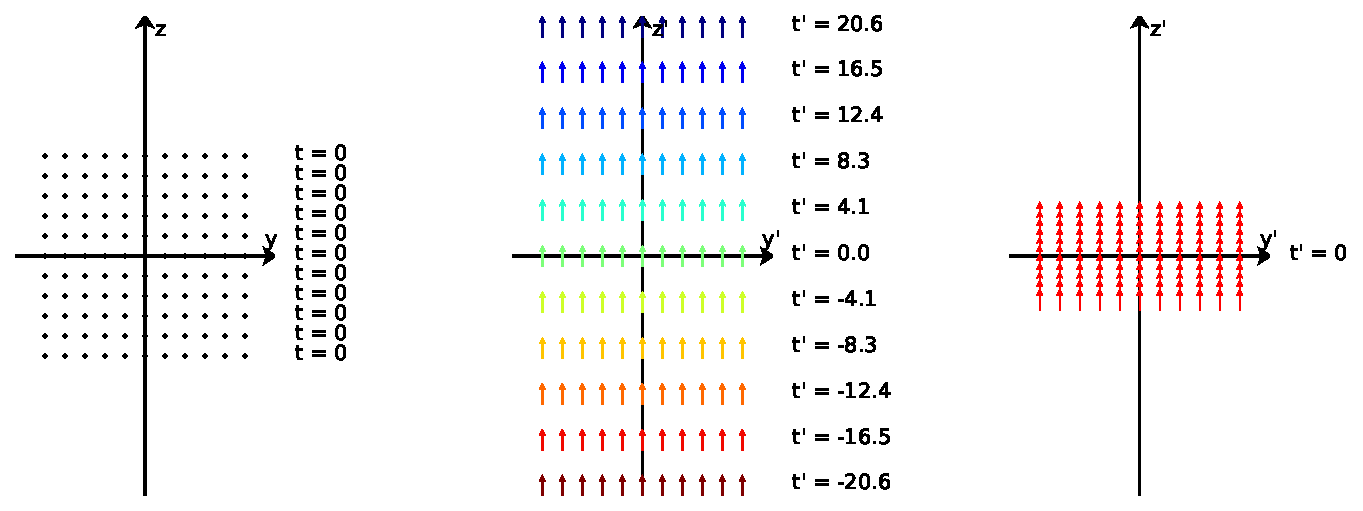
\includegraphics[width=10cm]{coordinate_transforms.pdf}
    \caption{Caption...}
    \label{fig: full coordinate transform}
\end{figure}
figure 1:
\hyperlink{def-proper-frame}{rest frame} of particles laid out in a grid at time $t=0$, with \hyperlink{def-observer}{observer} at origin
figure 2:
\hyperlink{def-Primed-Frame}{primed frame} $<S'>$ (\hyperlink{def-Primed-Frame}{primed frame} velocity is in negative z-direction, v=-0.9 ), with all coordinates transformed using \hyperlink{def-lorentz-transform}{Lorentz transformations} to the positions at time $t'=-\gamma \frac{zv}{c^2}$, and now have a velocity of -$v$  
figure 3:
Same \hyperlink{def-Primed-Frame}{primed frame} $<S'>$ but all particles are where they would be at time $t'=0$, i.e propagated forward or backwards from their current positions in time until they all have same time $t'=0$
figure 1:
Same \hyperlink{def-Primed-Frame}{primed frame} $<S'>$ but now with the particles positioned where they would be perceived to be my an \hyperlink{def-observer}{observer} at the origin with the \hyperlink{def-observer}{observer}s time $t'=0$, these positions are due to the delay in the light from these particles taking time to get to the \hyperlink{def-observer}{observer}, the \hyperlink{def-retarded-position}{retarded position} s of the particles.

%███████████████████████████████████████████████████████████████████
%███████████████████████████████████████████████████████████████████
\section{confusion between a frame change and looking at 2 different systems of moving objects TODO}


%███████████████████████████████████████████████████████████████████
%███████████████████████████████████████████████████████████████████
\section{Acceleration Transform TODO}

To find how the acceleration of a particle transforms for an \hyperlink{def-observer}{observer} in two different frames we take the differential of the velocity \hyperlink{def-transform}{transform} eq. \eqref{vector velocity transform} and use the differentiation rules for two generic functions $f$ and $g$: $d(gf)=f dg+g df$, and $d[f(g(x))]= dg(x) * df(g(x))$ 
\begin{equation}%%%%%%%%%%%%%%%
\begin{aligned}
     d\mathbf{U'} &= \dfrac{1}{\gamma\left(1- \dfrac{v}{c^2} u_z\right) }\begin{pmatrix}
    du_x \\ du_y  \\ \gamma du_z  \\
    \end{pmatrix} + \dfrac{\gamma \dfrac{v}{c^2} du_z}{\gamma^2\left(1- \dfrac{v}{c^2} u_z\right)^2 }\begin{pmatrix}
    u_x \\ u_y  \\ \gamma \left( u_z  - v  \right) \\
    \end{pmatrix}  \\
    &= ... \\
    &=  \dfrac{1}{\gamma\left(1- \dfrac{v}{c^2} u_z\right)^2 }\begin{pmatrix}
    du_x + \frac{v}{c^2}( u_x du_z - u_z du_x) \\ du_y + \frac{v}{c^2}( u_y du_z - u_z du_y) \\ \frac{1}{\gamma} du_z \\
    \end{pmatrix}
\end{aligned}      
\end{equation}%%%%
now dividing by the time differential from previous chapter to get the acceleration transform
\begin{equation}%%%%%%%%%%%%%%%
\mhl{
\begin{aligned}
     \mathbf{a'} =  \dfrac{1}{\gamma^2\left(1- \dfrac{v}{c^2} u_z\right)^3 }\begin{pmatrix}
    a_x + \frac{v}{c^2}(u_x a_z - u_z a_x) \\ a_y + \frac{v}{c^2}(u_y a_z - u_z a_y) \\ \frac{1}{\gamma} a_z \\
    \end{pmatrix}
    \\
    \text{at position $\mathbf{R'}$ and time $t'$ } 
\end{aligned}   
    }
\end{equation}%%%%

%███████████████████████████████████████████████████████████████████
\subsection{Generalised Acceleration Transform}

3 acceleration (check this)
\begin{equation}%%%%%%%%%%%%%%%
    \mathbf{a^{'}} = \frac{1}{\gamma ^3 \left(1-\frac{(\mathbf{u}\cdot \mathbf{v})}{c^2}\right)^3}\left[ \gamma  \left(1-\frac{(\mathbf{u}\cdot\mathbf{v})}{c^2}\right)\mathbf{a}+\frac{\gamma (\mathbf{a}\cdot\mathbf{v})}{c^2}\mathbf{u} + (1-\gamma ) (\mathbf{a}\cdot\hat{\mathbf{v}}) \cdot\hat{\mathbf{v}}\right]
\end{equation}%%%%
at position $\mathbf{R'}$ and time $t'$ 

%███████████████████████████████████████████████████████████████████
%███████████████████████████████████████████████████████████████████
\section{Variables}

$\vec{U_p}$ \newline

$\vec{V}$ \newline

$\vec{u}, \vec{v}$ \newline

$u_x, u_y, u_z$ \newline

$R_p$ \newline

$R$  \newline

$R'$ \newline

$dx dy dz dt$ \newline

$dx' dy' dz' dt'$ \newline

$dU$ \newline

$\vec{a} ax, ay, az$ \newline

$\hat{v}$ \newline




%███████████████████████████████████████████████████████████████████
%███████████████████████████████████████████████████████████████████
%███████████████████████████████████████████████████████████████████
\chapter{Spherical light pulses}
%███████████████████████████████████████████████████████████████████
%███████████████████████████████████████████████████████████████████
\section{Preliminary Math}
%███████████████████████████████████████████████████████████████████
\subsection{Spherical Polar Coordinates}


\tdplotsetmaincoords{60}{110}
\tikzsetnextfilename{Tikz_Spherical_Polar_Coordinates}
\begin{tikzpicture}[scale=3,tdplot_main_coords]
  % variables
  \def\rvec{.8}
  \def\thetavec{30}
  \def\phivec{60} 
  % axes
  \coordinate (O) at (0,0,0);
  \draw[thick,->] (0,0,0) -- (1,0,0) node[anchor=north east]{$x$};
  \draw[thick,->] (0,0,0) -- (0,1,0) node[anchor=north west]{$y$};
  \draw[thick,->] (0,0,0) -- (0,0,1) node[anchor=south]{$z$}; 
  % vectors
  \tdplotsetcoord{P}{\rvec}{\thetavec}{\phivec}
  \draw[-stealth,red] (O)  -- (P) node[above right] {$\mathbf{R}$};
  \draw[dashed,red]   (O)  -- (Pxy);
  \draw[dashed,red]   (P)  -- (Pxy);
  \draw[dashed,red]   (Py) -- (Pxy);
  % arcs
  \tdplotdrawarc[->]{(O)}{0.2}{0}{\phivec}
    {anchor=north}{$\phi$}
  \tdplotsetthetaplanecoords{\phivec}
  \tdplotdrawarc[->,tdplot_rotated_coords]{(0,0,0)}{0.5}{0}{\thetavec}
    {anchor=south west}{$\theta$}
\end{tikzpicture}

For a given coordinate $\mathbf{R}$ we have it shown how to get spherical polar coordinates $(r,\theta,\phi)$ from the Cartesian coordinates $(x,y,z)$, where $\theta \in [0,\pi] $ and $\phi \in [0,2\pi)$ are the angles from the Z-Axis and X-axis respectively, and $r$ is the distance from the origin, i.e. the magnitude

\begin{equation}%%%%%%%%%%%%%%%
\mhl{
    \mathbf{R} = \begin{pmatrix}
    x\\ y \\ z
    \end{pmatrix} =  r \begin{pmatrix}
    \cos{\phi}\sin{\theta}\\ \sin{\phi}\sin{\theta} \\ \cos{\theta}
    \end{pmatrix}      
    }
\end{equation}%%%%
with $r=\sqrt{x^2+y^2+z^2}$, $\phi=\arctan \frac{y}{x}$, and
$\theta=\arccos\frac{z}{r}=\arctan\frac{\sqrt{x^2+y^2}}{z}$

with the unit vectors for the spherical polar coordinates 

\begin{equation}%%%%%%%%%%%%%%%
   \mathbf{\hat{\text{$r$}}} = \begin{pmatrix}
  \sin\theta \, \cos\phi \\
 \sin\theta \, \sin\phi \\
 \cos\theta
\end{pmatrix},
\mathbf{\hat{\text{$\theta$}}} = \begin{pmatrix}
  \cos\theta \, \cos\phi \\
  \cos\theta \, \sin\phi \\
 - \sin\theta
\end{pmatrix},
\mathbf{\hat{\text{$\phi$}}} = \begin{pmatrix}
  - \, \sin\phi \\
 \hphantom{-} \, \cos\phi \\
 0
\end{pmatrix}
\end{equation}%%%%

\begin{equation}%%%%%%%%%%%%%%%
\begin{aligned}
    \frac{\partial\mathbf{R}}{\partial r} &= \mathbf{\hat{\text{$r$}}}\\ 
    \frac{\partial\mathbf{R}}{\partial \theta} &= \begin{pmatrix}
 r \cos\theta  \cos\phi \\
 r \cos\theta  \sin\phi \\
 -r \sin\theta
\end{pmatrix} =r\mathbf{\hat{\text{$\theta$}}} \\
    \frac{\partial\mathbf{R}}{\partial \phi} &= \begin{pmatrix}
 -r \sin\theta  \sin\phi \\
 r \sin\theta  \cos\phi \\
 0
\end{pmatrix} = r \sin\theta \mathbf{\hat{\text{$\phi$}}} 
\end{aligned}
\end{equation}%%%%





%███████████████████████████████████████████████████████████████████
\subsection{Surface element}


%Axis Angles  
\tdplotsetmaincoords{70}{110}

%Macros  
\pgfmathsetmacro{\rvec}{6}  
\pgfmathsetmacro{\thetavec}{40}  
\pgfmathsetmacro{\phivec}{45}

\pgfmathsetmacro{\dphivec}{20}  
\pgfmathsetmacro{\dthetavec}{20}  
\pgfmathsetmacro{\drvec}{1.5}

%Layers  
\pgfdeclarelayer{background} 
\pgfdeclarelayer{foreground}

\pgfsetlayers{background, main, foreground}

\tikzsetnextfilename{Tikz_Surface_Element}
\begin{tikzpicture}[tdplot_main_coords]
%
%Coordinates  
\coordinate (O) at (0,0,0);  
\tdplotsetcoord{A}{\rvec}{\thetavec}{\phivec}  
\tdplotsetcoord{B}{\rvec}{\thetavec + \dthetavec}{\phivec}         
\tdplotsetcoord{C}{\rvec}{\thetavec + \dthetavec}{\phivec + \dphivec}  
\tdplotsetcoord{D}{\rvec}{\thetavec}{\phivec + \dphivec}  
\tdplotsetcoord{E}{\rvec + \drvec}{\thetavec}{\phivec}  
\tdplotsetcoord{F}{\rvec + \drvec}{\thetavec + \dthetavec}{\phivec}  
\tdplotsetcoord{F'}{\rvec + \drvec}{90}{\phivec}  \tdplotsetcoord{G}{\rvec + \drvec}{\thetavec + \dthetavec}{\phivec + \dphivec}  
\tdplotsetcoord{G'}{\rvec + \drvec}{90}{\phivec + \dphivec} 
\tdplotsetcoord{H}{\rvec + \drvec}{\thetavec}{\phivec + \dphivec} 
%  
%Axis  
\begin{pgfonlayer}{background}  
\draw[thick,-latex] (0,0,0) -- (7,0,0) node[pos=1.1]{$x$};        
\draw[thick,-latex] (0,0,0) -- (0,7,0) node[pos=1.05]{$y$};         
\draw[thick,-latex] (0,0,0) -- (0,0,6) node[pos=1.05]{$z$};                   
\end{pgfonlayer}
%
%Help Lines  
\begin{pgfonlayer}{background}  
%Up     
\draw[thick, blue] (O) -- (A) node[pos=0.6, above left, blue] {$r$};    
\draw (O) -- (B);   
\draw (O) -- (C);   
\draw[dashed] (O) -- (D);   
%Down   
\draw (O) -- (F');  
\draw (O) -- (G');  
\end{pgfonlayer}  
\begin{pgfonlayer}{foreground}  
%%Help Curves   
\tdplotsetthetaplanecoords{\phivec}     
\tdplotdrawarc[tdplot_rotated_coords]{(O)}{\rvec}{\thetavec+\dthetavec}{90}{}{}
%
\tdplotdrawarc[tdplot_rotated_coords]{(O)}{\rvec+\drvec}{\thetavec+\dthetavec}{90}{}{}
%
\tdplotsetthetaplanecoords{\phivec+\dphivec}    
\tdplotdrawarc[tdplot_rotated_coords, dashed]{(O)}{\rvec}{\thetavec+\dthetavec}{90}{}{}     
\tdplotdrawarc[tdplot_rotated_coords]{(O)}{\rvec+\drvec}{\thetavec+\dthetavec}{90}{}{}
%   
\tdplotdrawarc[tdplot_main_coords]{(O)}{\rvec}{\phivec}{\phivec+\dphivec}{}{}
%    
\tdplotdrawarc[tdplot_main_coords]{(O)}{\rvec+\drvec}{\phivec}{\phivec+\dphivec}{below, rotate=13}{$r\sin\theta\mathrm{d}\phi$} 
\end{pgfonlayer}
%
%Angles  
\begin{pgfonlayer}{foreground}  
%Phi, dPhi  
\tdplotdrawarc[-stealth]{(O)}{0.9}{0}{\phivec}{anchor=north}{$\phi$}    
\tdplotdrawarc[-stealth]{(O)}{1.5}{\phivec}{\phivec + \dphivec}{}{}     
\node at (1.4,1.9,0) {$\mathrm{d}\phi$};        
\tdplotsetthetaplanecoords{\phivec}     
%Theta, dTheta          
\tdplotdrawarc[tdplot_rotated_coords,-stealth]{(0,0,0)}{1.2}{0}{\thetavec}{}{}      
\node at (0,0.3,1.3) {$\theta$};    
\tdplotdrawarc[tdplot_rotated_coords,-stealth]{(0,0,0)}{2.5}{\thetavec}{\thetavec + \dthetavec}{anchor=south west}{$\mathrm{d}\theta$}  
\end{pgfonlayer}
%
%Differential Volume
%
%%Lines  
\begin{pgfonlayer}{foreground}  
\draw[thick] (A) -- (E) node[midway, above left]{$\mathrm{d}r$};    
\draw[thick] (B) -- (F);    
\draw[thick] (C) -- (G);      
\end{pgfonlayer}   
\begin{pgfonlayer}{background}
\draw[dashed, thick] (D) -- (H);  
\end{pgfonlayer}
%
%%Curved 
\begin{pgfonlayer}{background}      
\tdplotsetrotatedcoords{55}{-50.4313}{-6.4086}  
\tdplotdrawarc[dashed, tdplot_rotated_coords, thick]{(O)}{\rvec}{0}{12.8173}{}{}
%   
\tdplotsetthetaplanecoords{\phivec + \dphivec}  
\tdplotdrawarc[dashed, tdplot_rotated_coords, thick]{(O)}{\rvec}{\thetavec}{\dthetavec + \thetavec}{}{}  
\end{pgfonlayer} 
\begin{pgfonlayer}{foreground}     
\tdplotsetthetaplanecoords{\phivec}     
\tdplotdrawarc[tdplot_rotated_coords, thick]{(O)}{\rvec}{\thetavec}{\dthetavec + \thetavec}{}{}     
\tdplotdrawarc[tdplot_rotated_coords, thick]{(O)}{\rvec + \drvec}{\thetavec}{\dthetavec + \thetavec}{}{}
%   
\tdplotsetthetaplanecoords{\phivec + \dphivec}  
\tdplotdrawarc[tdplot_rotated_coords, thick]{(O)}{\rvec + \drvec}{\thetavec}{\dthetavec + \thetavec}{above right}{$r\mathrm{d}\theta$}  
%   
\tdplotsetrotatedcoords{55}{-50.4313}{-6.4086}  
\tdplotdrawarc[tdplot_rotated_coords, thick]{(O)}{\rvec + \drvec}{0}{12.8173}{}{}   
%   
\tdplotsetrotatedcoords{55}{-30.3813}{-8.6492}    %     
\tdplotdrawarc[tdplot_rotated_coords, thick]{(O)}{\rvec}{0}{17.2983}{}{}    
\tdplotdrawarc[tdplot_rotated_coords, thick]{(O)}{\rvec + \drvec}{0}{17.2983}{}{}  
\end{pgfonlayer}
%
%Fill Color 
\begin{pgfonlayer}{main}    
    %Front  
    \fill[black, opacity=0.15] (E) to (A)  to[bend left=4] (B) to (F) to[bend right=4] cycle;   
    \fill[black, opacity=0.6] (E) to[bend left=4] (F)  to[bend left=2] (G) to[bend right=6.5] (H) to[bend right=4] cycle;   
    \fill[black, opacity=0.4] (F) to[bend left=2] (G) to[bend left=1.5] (C) to[bend right=2.5] (B) to[bend right=4] cycle;   
\end{pgfonlayer}  
\begin{pgfonlayer}{background}  
    %Back   
    \fill[black!50, opacity=0.5] (A) to[bend left=2] (D) to[bend left=6] (C) to[bend right=2.5] (B) to[bend right=4] cycle;     
    \fill[black!50, opacity=0.5] (A) to[bend left=2] (D) to (H) to[bend right=2.5] (E) to[bend right=4] cycle;  
    \fill[black!50, opacity=0.5] (D) to (H) to[bend left=6] (G) to[bend right=2] (C) to[bend right=6] cycle;  
\end{pgfonlayer}
\end{tikzpicture}




The surface element spanning from $\theta$ to $\theta + d\theta$ and $\phi$ to $\phi + d\phi$ on a spherical surface at (constant) radius r is then
\begin{equation}%%%%%%%%%%%%%%%
    \mathrm{d}S =
 \left\|\frac{\partial {\mathbf R}}{\partial \theta} \times \frac{\partial {\mathbf R}}{\partial \phi}\right\| \mathrm{d}\theta \,\mathrm{d}\phi = \left| r \mathbf{\mathbf{\hat{\text{$\theta$}}}} \times r \sin \theta \mathbf{\mathbf{\hat{\text{$\phi$}}}} \right|= r^2 \sin\theta \,\mathrm{d}\theta \,\mathrm{d}\phi
\end{equation}%%%%

The differential solid angle is
\begin{equation}%%%%%%%%%%%%%%%
    \mathrm{d}\Omega = \frac{\mathrm{d}S}{r^2} = \sin\theta \,\mathrm{d}\theta \,\mathrm{d}\phi
\end{equation}%██████

A solid angle $\Omega$ is a measure of the amount of the field of view from some particular point that a given object covers. 
The fraction of the field of view covered from a point is given by $\Omega/ 4\pi$



%███████████████████████████████████████████████████████████████████
%███████████████████████████████████████████████████████████████████
\section{Light Speed Transform}
for the case where the speed is that of light, $|u|=c$, with the direction in first frame is at an angle $\alpha$ from the z-axis and $\varphi$, so that in spherical polar coordinates

\begin{equation}%%%%%%%%%%%%%%%
    \mathbf{c} = c \begin{pmatrix}
    \cos{\varphi}\sin{\alpha}\\ \sin{\varphi}\sin{\alpha} \\ \cos{\alpha}
    \end{pmatrix},
\end{equation}%%%%
we then have from the velocity \hyperlink{def-transform}{transform} in Eq. \eqref{vector velocity transform}

% \begin{equation}%%%%%%%%%%%%%%%
%     \begin{aligned}
%       & u'_x =\frac{c\sin\alpha\cos\varphi}{\gamma \bigg(1-\frac{v\cos\alpha}{c}\bigg) } \\ & u'_y =\frac{c\sin\alpha\sin\varphi}{\gamma \bigg(1-\frac{v\cos\alpha}{c}\bigg) } \\ & u'_z =\frac{c\cos\alpha -v}{ \bigg(1-\frac{v\cos\alpha}{c}\bigg) }
%     \end{aligned}
% \end{equation}%██████

\begin{equation}%%%%%%%%%%%%%%%
\label{light speed velocity transform}
\mhl{
\begin{aligned}
     &\mathbf{c'} = \dfrac{c}{\gamma\left(1- \dfrac{v}{c} \cos\alpha\right) }\begin{pmatrix}
    \sin\alpha\cos\varphi  \\ \sin\alpha\sin\varphi  \\ \gamma \left( \cos\alpha  - \dfrac{v}{c}  \right) \\
    \end{pmatrix}  \\
    &\text{at position $\mathbf{R'}$ and time $t'$ } 
\end{aligned}      
    }
\end{equation}%%%%

which still has the same speed of light (can be shown easily by taking magnitude of vector) but has rotated / aberrated propagation angle. \newline
Speed of light: (easy mistake: speed of light is constant, not the velocity as direction of movement does change)\newline



%███████████████████████████████████████████████████████████████████
%███████████████████████████████████████████████████████████████████
\section{Special Relativistic Aberration}
%███████████████████████████████████████████████████████████████████
\subsection{Setup of Spherical light Pulse}

In the \hyperlink{def-proper-frame}{rest frame} of a point source particle positioned at the origin $O = (0,0,0)$ and at time $t=0$ we have a spherical pulse of light emanated from the source, which is propagated at velocity $\mathbf{c}$ (from last section) in all direction 

for a time $t=T_{prop} \geq 0$, so that the position of any part of the light pulse is given as 
\begin{equation}%%%%%%%%%%%%%%%
\label{displacement: proper pulse}
    \mathbf{R} =  c t \begin{pmatrix}
    \cos{\varphi}\sin{\alpha}\\ \sin{\varphi}\sin{\alpha} \\ \cos{\alpha}
    \end{pmatrix}.
\end{equation}%%%%

\begin{figure}[ht]
\centering
       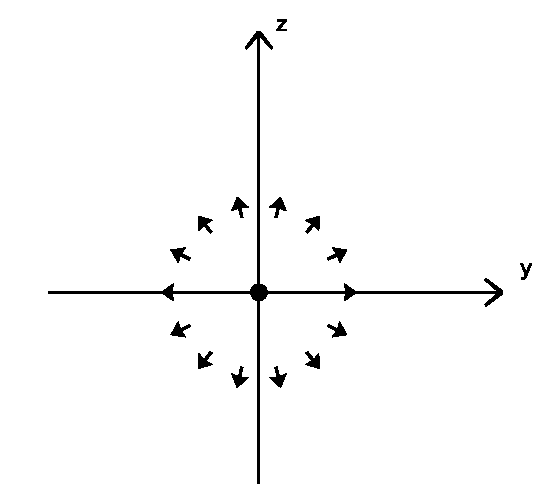
\includegraphics[width=6cm]{Rest_Pulse.pdf}
    \caption{Diagram showing, position of light pulse after a certain amount time}
    \label{fig: Rest Pulse}
\end{figure}

%███████████████████████████████████████████████████████████████████
\subsection{Aberration}

Now changing to a \hyperlink{def-Primed-Frame}{primed frame}, moving at speed $v$ in the z-direction, relative to the sources \hyperlink{def-proper-frame}{rest frame}

The \hyperlink{def-lorentz-transform}{Lorentz transformations} of the spacial and time coordinates gives the primed positions of the light pulse to be

\begin{equation}%%%%%%%%%%%%%%%
\label{displacement: primed pulse}
    \mathbf{R'} = c t \begin{pmatrix}
    \cos{\varphi}\sin{\alpha}\\ \sin{\varphi}\sin{\alpha} \\ \gamma\left(\cos{\alpha} - \dfrac{v}{c}\right)
    \end{pmatrix},
\end{equation}%%%%
at primed time 
\begin{equation}%%%%%%%%%%%%%%%
    t' = \gamma \left(t - \dfrac{v}{c^2}ct\cos{\alpha}\right) =  \gamma \left(1 - \frac{v}{c} \cos{\alpha}\right) t 
\end{equation}%%%%

\begin{figure}[H]
\centering
       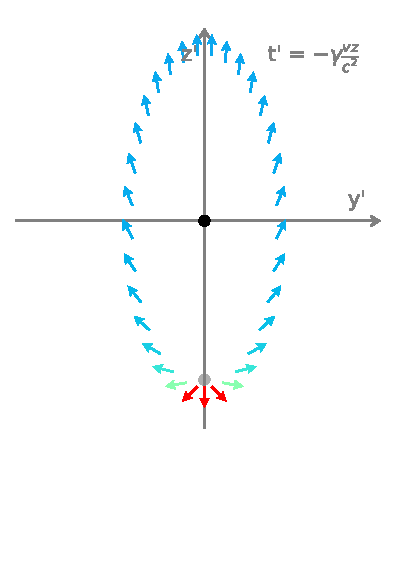
\includegraphics[width=8cm]{Prime_Pulse.pdf}
    \caption{*** since have better images, these are same pulse, the elipsoid has its pulse transformed to it at different times, and the circular pulse is when you account for this and propagate each part of the pulse, to back or forward in time so that each part has the same time}
    \label{fig: Prime Pulse}
\end{figure}

*** Here you can see that this primed propagation velocity is in the same direction as the primed displacement vector, the \hyperlink{def-Primed-Frame}{primed frame}s origin is located at the location the pulse was emitted from \newline
*** $v=-u_p$ 


\begin{figure}[ht]
\centering
       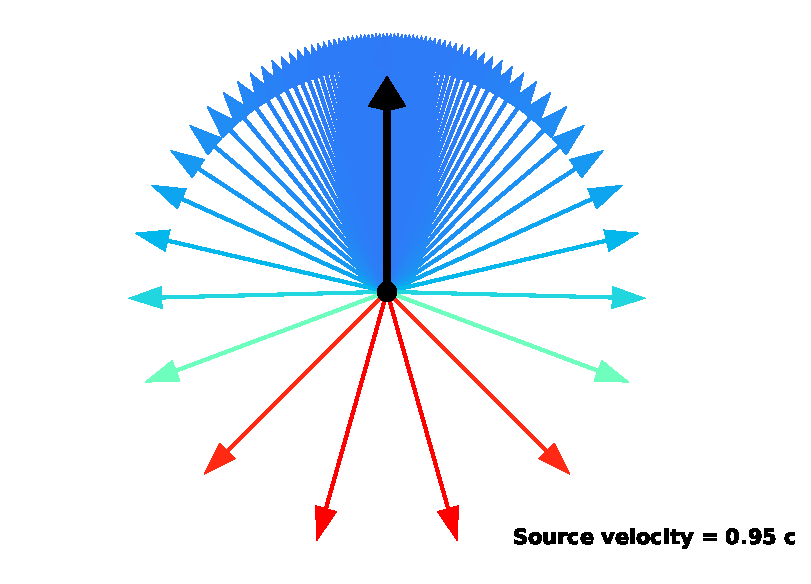
\includegraphics[width=8cm]{Aberrated_velocities.pdf}
    \caption{primed velocities of a evenly distributed pulse of light in \protect\hyperlink{def-proper-frame}{rest frame} of the source}
    %\label{fig: label}
\end{figure}

say about particles approaching speed of light emitting light only in the direction its moving at the speed its moving

*** some diagrams with inward coming light ***
and what math is changed from before



The propagation directions of the light as seen in figure (REF), are transformed such that the angles between them and the Z-Axis, have the aberrational relationship
\begin{equation}%%%%%%%%%%%%%%%
\label{Cosine transform}
\mhl{
    \cos\theta' = \frac{\mathbf{U}'_z}{\|\mathbf{U}'\|} \equiv \frac{\mathbf{R}'_{z}}{\|\mathbf{R}'\|} =  \dfrac{\cos\theta + \dfrac{u_p}{c}}{1+\dfrac{u_p}{c}\cos\theta}.
    }
\end{equation}%%%%
This is the relativistic aberration formula \cite{einstein1905electrodynamics}, it shows how the field's propagation direction transforms

%███████████████████████████████████████████████████████████████████
%███████████████████████████████████████████████████████████████████
\section{Variables}

$\theta, \phi, R$ \newline

$r$ \newline

$\hat{r}$ \newline

$\hat{\theta}$ \newline

$\hat{\phi}$ \newline

$dS$ \newline

$d\Omega$ \newline

$\Omega$ \newline

$\varphi, \alpha,$  \newline

$u_p$ \newline


%███████████████████████████████████████████████████████████████████
%███████████████████████████████████████████████████████████████████
%███████████████████████████████████████████████████████████████████
\chapter{Beaming of light}

%███████████████████████████████████████████████████████████████████
%███████████████████████████████████████████████████████████████████
\section{Delay in Light-Speed Signals}

Light travels extremely fast (roughly 300,000,000 m/s) compared to other everyday speeds we are used to. In the blink on an eye light could travel around the world twice. So we don't need to normally worry about the delay in the light signal, as the time to propagate the distances in our everyday world is very short, we can normally assume an instantaneous signal, and ignore the more complex modelling of the delayed signal. But when it comes to particle physics were the particles or astronomy where we might be dealing with speeds close to that of light and also huge distances, e.g. light has take 152,000 years to travel from the Andromeda galaxy, so we are currently seeing this galaxy where it was and how it looked 152,000 years ago. These past positions that we currently see are called the \hyperlink{def-retarded-position}{retarded position} s/delayed view. 

\newpage

%███████████████████████████████████████████████████████████████████
%███████████████████████████████████████████████████████████████████
\section{Transform of Light Pulse from Origin}

\begin{figure}[ht]
\begin{subfigure}{.49\textwidth} 
  \tikzsetnextfilename{Tikz_Light_Pulse_Proper_Frame}
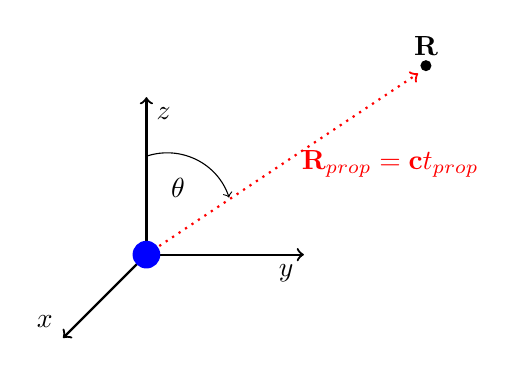
\begin{tikzpicture}[scale=5] %[,tdplot_main_coords]
%\usetikzlibrary{arrows.meta}
\draw[black, thick,->] (0,0,0) -- (0.4,0,0) node[anchor=north east]{$y$};
\draw[black, thick,->] (0,0,0) -- (0,0.4,0) node[anchor=north west]{$z$};
\draw[black, thick,->] (0,0,0) -- (0,0,0.55) node[anchor=south east] {$x$};
\node at (0.08,0.17,0) {$\theta $};
\draw[->] (0,0.25,0) to[bend left=45] (0.21,0.145,0);
\draw[thick,red, dotted,->] (0,0,0) -- (0.69,0.46,0) node[midway , right] {\text{ $ \mathbf{R}_{prop}=\mathbf{c} t_{prop}$}};
\fill[blue] (0,0,0) circle (1pt);
\fill[black] (0.71,0.48,0) circle (0.4pt) node[above] {\text{$ \mathbf{R}$}};
\end{tikzpicture}
\caption{\hyperlink{def-proper-frame}{proper frame}}
\label{fig: proper frame 1}
\end{subfigure}
\begin{subfigure}{.49\textwidth}
  \tikzsetnextfilename{Tikz_Light_Pulse_Primed_Frame}
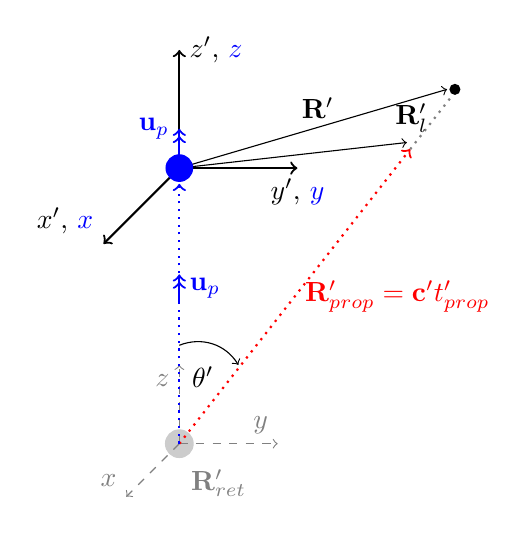
\begin{tikzpicture}[scale=5] %[,tdplot_main_coords]
%\usetikzlibrary{arrows.meta}
%node[anchor = north west]{\textcolor{black}{  $\mathbf{P}'$}}; %$\mathbf{P}'$}};
\node[gray] at (0.1,-0.1,0) {$\mathbf{R}'_{ret}$};
\draw[gray!40,fill=gray!40] (0,0,0) circle (1pt);
\draw[black, thick,->] (0,0.7,0) -- (0.3,0.7,0) node[anchor=north]{$y'$, {\color{blue} $y$}};
\draw[black, thick,->] (0,0.7,0) -- (0,1,0) node[anchor=west]{$z'$, {\color{blue} $z$}};
\draw[black, thick,->] (0,0.7,0) -- (0,0.7,0.5) node[anchor=south east] {$x'$, {\color{blue} $x$}};
\draw[gray, dashed,->] (0,0,0) -- (0.25,0,0) node[anchor=south east]{$y$};
\draw[gray, dashed,->] (0,0,0) -- (0,0.2,0) node[anchor=north east]{$z$};
\draw[gray, dashed,->] (0,0,0) -- (0,0,0.35) node[anchor=south east] {$x$}; 
\node at (0.06,0.17,0) {$\theta '$};
\draw[->] (0,0.25,0) to[bend left=40] (0.15,0.2,0);
\draw[red, thick, dotted,->] (0,0,0) -- (0.69*0.85,0.88*0.85,0) node[midway, right] {$\mathbf{R}'_{prop}=\mathbf{c'} t'_{prop}$};
\draw[gray, thick, dotted] (0.69*0.85,0.88*0.85,0) -- (0.69,0.88,0);
\draw[black,->] (0,0.7,0) -- (0.68,0.9,0) node[midway,above] {\text{ $\mathbf{R}'$}};
\draw[black,->] (0,0.7,0) -- (0.68*0.85,0.9*0.85,0) node[above] {\text{ $\mathbf{R}'_{l}$}};
\fill[blue] (0,0.7,0) circle (1pt);
\draw[thick,blue,dotted,->] (0,0,0) -- (0,0.66,0);
\draw[blue, thick,->>] (0,0.7,0) -- (0,0.8,0) node[left]{$\mathbf{u}_p$};
\fill (0.7,0.9,0) circle (0.4pt);
\draw[blue, thick,->>] (-0,0.36,0) -- (-0,0.43,0) node[midway, right]{$\mathbf{u}_p$};
\end{tikzpicture}
\caption{\hyperlink{def-Primed-Frame}{primed frame} with moving source}
\label{fig: primed frame 1}
\end{subfigure}
\caption{ The diagram shows a particle $p$ in blue at rest in the \protect\hyperlink{def-proper-frame}{proper frame}, Fig (a), with a light pulse that has propagated along $\mathbf{R}_{prop}$ shown in red, at an angle $\theta$ from the z-axis, to coordinate $\mathbf{R}$ shown in black, with the current time for whole system being $t=0$.
Fig (b), shows the system transformed to a \protect\hyperlink{def-Primed-Frame}{primed frame} moving at velocity $\mathbf{v}=(0,0,v)$ in the z-direction relative to the \protect\hyperlink{def-proper-frame}{proper frame}, such that the particle and its attached proper axis in this frame are moving at velocity $\mathbf{u}_p= - \mathbf{v}$ and is currently at the origin with time $t'=0$. when the light was emitted from the particle, they were at the \protect\hyperlink{def-retarded-position}{retarded position}  $\mathbf{R}'_{ret}$ shown in grey, this light was then propagated at an angle $\theta'$ from the z-axis, along $\mathbf{R}'_{prop}$ to reach $\mathbf{R}'_{l}$ at $t'=0$. it has not yet reached the corresponding \protect\hyperlink{def-lorentz-transform}{Lorentz transformed} coordinate $\mathbf{R}'$ }
\label{fig: Retarded field outward field transform}
\end{figure}



As visualised in figure (\ref{fig: Retarded field outward field transform}). If we have a light source particle $p$, in its \hyperlink{def-proper-frame}{rest frame} that had emitted a pulse of light in one such that it propagates along $\mathbf{R}_{prop}=\mathbf{c}t_{prop}$ at an angle $\theta$ from the z-axis and is currently at position $\mathbf{R}$ at time $t=0$, where $\mathbf{c}$ is the velocity of light and $t_{prop}$ is the time it took to propagate to $\mathbf{R}$.
This system is then transformed as follows; the coordinate $\mathbf{R}$ is transformed to 
\begin{equation}%%%%%%%%%%%%%%%
\label{displacement transform}
    \mathbf{R'} =   \begin{pmatrix}
    x\\ y \\ \gamma z
    \end{pmatrix},
\end{equation}%%%%

the light pulse's velocity using eq. (REF) in Cartesian coordinates and particles speed in the \hyperlink{def-Primed-Frame}{primed frame} $u_p=-v$
\begin{equation}%%%%%%%%%%%%%%%
\label{light pulse velocity transform}
    \mathbf{c'} =  \dfrac{c}{\text{\AA}} \begin{pmatrix}
    \frac{x}{\|\mathbf{R}\|}\\ \frac{y}{\|\mathbf{R}\|} \\ \gamma \left( \frac{z}{\|\mathbf{R}\|} + \dfrac{u_p}{c} \right)
    \end{pmatrix}
\end{equation}%%%%

The time that the particle emits the light in the \hyperlink{def-proper-frame}{proper frame} is $t_{ret}= - \frac{||\mathbf{R}_{prop}||}{||\mathbf{c}||}$ which corresponds to the time
\begin{equation}%%%%%%%%%%%%%%%
    t'_{ret}= \gamma t_{ret} = - \gamma \frac{||\mathbf{R}_{prop}||}{||\mathbf{c}||}
\end{equation}%%%%
then in the \hyperlink{def-Primed-Frame}{primed frame}, the \hyperlink{def-retarded-position}{retarded position}  at which the particle emmits the light pulse is
\begin{equation}%%%%%%%%%%%%%%%
    \mathbf{R'}_{ret} = - \gamma \frac{||\mathbf{R}_{prop}||}{||\mathbf{c}||} \mathbf{u}_p
\end{equation}%%%%

to find the position the light pulse is currently at, at time $t'=0$, we have to rewind its time from the position $\mathbf{R}'$ that its at when using the \hyperlink{def-lorentz-transform}{Lorentz transform} at time $t'= -\gamma\frac{vz}{c^2}= \gamma\frac{u_p z}{c^2}$ taking away the displacement it propagated in this time to get the current position of light to be (($t'_{prop} = - t'_{ret}$))
\begin{equation}%%%%%%%%%%%%%%%
\begin{split}
    \mathbf{R'}_l &= \mathbf{R'}_{ret} + \mathbf{c'}t'_{prop} = \left( \mathbf{u}_p - \mathbf{c}' \right)t'_{ret} \\
    &= \gamma \frac{||\mathbf{R}||}{\text{\AA}} 
    \begin{pmatrix}
    \frac{x}{||\mathbf{R}||}\\  \frac{y}{||\mathbf{R}||} \\ \gamma \left( \frac{z}{||\mathbf{R}||} +\frac{u_p}{c}\right) - \text{\AA}\frac{u_p}{c}
    \end{pmatrix} 
    = ...\\
    &= \frac{1}{\text{\AA}} 
    \begin{pmatrix}
    \gamma x\\  \gamma y \\ z
    \end{pmatrix}     
\end{split}
\end{equation}%%%%

we have the ratio of the propagation distance as

\begin{equation}%%%%%%%%%%%%%%%
    \dfrac{||\mathbf{R}'_{prop}||}{||\mathbf{R}_{prop}||} = \dfrac{t'_{prop}}{t_{prop}} = \gamma
\end{equation}%%%%

%███████████████████████████████████████████████████████████████████
\subsection{Doppler Effect (to come back to)}

%██████████
\begin{figure}[ht]
\begin{subfigure}{.49\textwidth}
\centering
  \tikzsetnextfilename{Tikz_Lights_angle_with_particle_With_particle_moving}
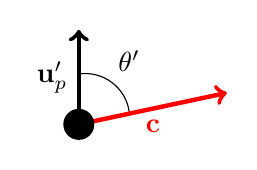
\begin{tikzpicture}[scale=8] 
\draw[-] (0,0.08,0) to[bend left=45] (0.08,0.02,0);
\node at (0.08,0.1,0) {$\theta' $};
\draw[red,ultra thick, ->] (0,0,0) -- (0.235,0.05,0) node[midway,anchor= north]{$\mathbf{c}$};
\draw[ultra thick, ->] (0,0,0) -- (0,0.15,0)node[midway,anchor=east]{$\mathbf{u}'_p$};
\fill[black] (0,0,0) circle (0.7pt);
\end{tikzpicture}
\caption{Light travelling relative to moving particle}
%  \label{fig:sub1}
\end{subfigure}
\begin{subfigure}{.49\textwidth}
\centering
\tikzsetnextfilename{Tikz_Lights_angle_with_particle_in_its_proper_frame}
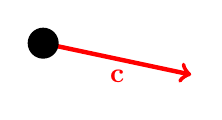
\begin{tikzpicture}[scale=8] 
\draw[red,ultra thick, ->] (0,0,0) -- (0.235,-0.05,0) node[midway,anchor= north]{$\mathbf{c}$};
\fill[black] (0,0,0) circle (0.7pt);
\end{tikzpicture}
\caption{Light travelling relative to particle when at rest}
%  \label{fig:sub2}
\end{subfigure}
\caption{ light being absorbed by moving and rest particles}
\label{fig: Doppler effect}
\end{figure}
%██████████

For a particle $p$ at rest emitting wave at light speed in any direction, we have the length the wave has travelled in time $d\tau$ as being $cd\tau$.
If we have a particle $p$ moving at speed $u'_p$ in the z-direction and wave being emitted in all directions from it, we have the wave emitted at an angle $\alpha$ from the z-axis, travelling distance $cdt$ in a time $dt$, with the particle moving a distance $ u'_p \cos\alpha dt$ in the direction of this emitted part of the wave, this leads to a bunching up of the wave in the direction of the movement of the particle ($cdt - u'_p \cos\alpha dt= (1-\frac{u'_p}{c}\cos\alpha)cdt$, the ratio of space the wave takes up in that direction compared to the \hyperlink{def-proper-frame}{rest frame} is 
\begin{equation}
    Ratio = \frac{ \gamma \left(1-\dfrac{u'_p}{c}  \cos\theta \right) c dt}{c d\tau}
\end{equation}
since as wavelength is inversely proportional to the frequency, and this bunching up at the front will proportionally decrease the wavelength
\begin{equation}
    \Phi_r = \frac{c d\tau}{ \gamma \left(1-\dfrac{u'_p}{c}  \cos\theta \right) c dt} 
\end{equation}
with rate of change in time flow for both frames having the relation $dt=\gamma d\tau$ we get the ratio of this
\begin{equation}
    \Phi_r = \frac{1}{ \gamma \left(1-\dfrac{u'_p}{c}  \cos\theta \right)} 
\end{equation}
the vector cosine relation is $\cos\alpha = \frac{\mathbf{u}'_p \cdot \mathbf{c}}{u'_p c}$, giving 
\begin{equation}
    \Phi_r = \frac{1}{ \gamma \left(1-\dfrac{\mathbf{u}'_p \cdot \mathbf{c}}{ c^2} \right)} 
\end{equation}
%███████████████████████████████████████████████████████████████████
\subsection{Relativistic beaming or Flux from Point Source}

A \hyperlink{def-proper-frame}{proper frame} of a particle's differential solid angle element  (definition given in previous chapter (maybe move that subsection to here))
\begin{equation}%%%%%%%%%%%%%%%
    d\Omega = \sin{\theta} d\theta d\phi,
\end{equation}%%%%
encompasses a certain amount of the wavefront, this is the same amount of the wavefront that is encompassed by the coinciding aberrated differential solid angle
\begin{equation}%%%%%%%%%%%%%%%
    d\Omega' = \sin{\theta'} d\theta' d\phi'.
\end{equation}%%%%
We can calculate this element by differentiating both sides of equation \eqref{Cosine transform} with respect to $\theta$ \cite{hogg1997special}, which gives
\begin{equation}%%%%%%%%%%%%%%%
    \sin{\theta'} d\theta' =   \dfrac{1-\dfrac{u_p^2}{c^2}}{\left(1+\dfrac{u_p}{c}\cos{\theta}\right)^2} \sin{\theta} d\theta =  \dfrac{1}{\gamma^2\left(1+\dfrac{u_p}{c}\cos{\theta}\right)^2} \sin{\theta} d\theta
\end{equation}%%%%
as $v=-u_p$ now using this and $d\phi'=d\phi$ (as the angle $\phi$ is always perpendicular to the motion of the particle and hence unaffected by \hyperlink{def-transform}{transformation} ) we have the solid angle in the \hyperlink{def-Primed-Frame}{primed frame} given as
\begin{equation}%%%%%%%%%%%%%%%
\mhl{
    d\Omega' = \dfrac{1}{\gamma^2\left(1+\dfrac{u_p}{c}\cos{\theta}\right)^2} \sin{\theta} d\theta d\phi.
    }
\end{equation}%%%%
%The overall amount of wavefront is conserved, as can be seen when integrating over the corresponding solid angle in either frame, both of which gives the same value of $4\pi$.
%  proportional to the amount of the wavefront in the given proper differential element of the solid angle, and
The relative primed wavefront strength at a given angle is taken as being proportional to the amount of the wavefront per solid angle in the \hyperlink{def-Primed-Frame}{primed frame} relative to that in the \hyperlink{def-proper-frame}{proper frame}, referred to here as the aberrational wavefront strength weighting, given as
\begin{equation}%%%%%%%%%%%%%%% 
\label{eq: aberrational wavefront weighting}
    \Phi_\Omega = \frac{d\Omega}{d\Omega'} = \text{\AA}^2.
\end{equation}%%%%
(define what i mean by strength weighting)

%███████████████████████████████████████████████████████████████████
\subsection{Relativistic Beaming of Multiple Wave Fronts of Light}

Both of the previous effects can be seen more clearly when looking at how multiple pulses of spherically evenly distributed light \hyperlink{def-transform}{transform} 
\begin{figure}[ht]
\centering
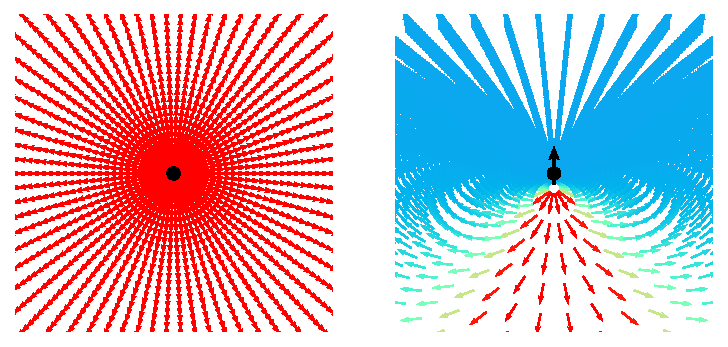
\includegraphics[width=10cm]{Still_Retarded_Field_Both_Frames.pdf}
    \caption{A 2D diagram showing multiple spherically symmetrical pulses of light from a source at rest  (left), and in a corresponding primed inertial frame where the source is moving (right), the colours show the \protect\hyperlink{def-doppler-effect}{Doppler effect} on lights light}
    \label{fig: full field transformation}
\end{figure}

%███████████████████████████████████████████████████████████████████
%███████████████████████████████████████████████████████████████████
\section{Relativistic Retarded view of universe for an observer}

\begin{figure}[ht]
\begin{subfigure}[b]{.49\textwidth}
  \tikzsetnextfilename{Tikz_Particles_position_in_rest_frame}
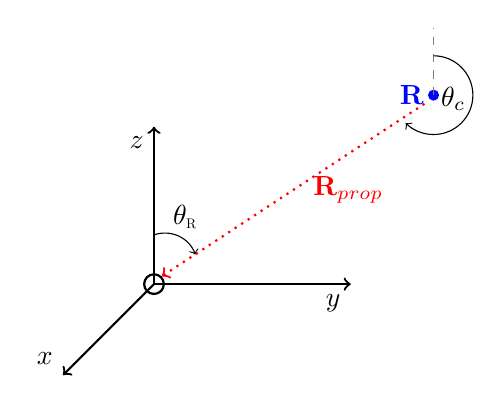
\begin{tikzpicture}[scale=5] %[,tdplot_main_coords]
%\usetikzlibrary{arrows.meta}
\draw[thick] (0 ,0) circle (0.025);
\draw[black, thick,->] (0,0,0) -- (0.5,0,0) node[anchor=north east]{$y$};
\draw[black, thick,->] (0,0,0) -- (0,0.4,0) node[anchor=north east]{$z$};
\draw[black, thick,->] (0,0,0) -- (0,0,0.6) node[anchor=south east] {$x$};
\draw[->] (0,0.25/2,0) to[bend left=45] (0.21/2,0.15/2,0);
\node at (0.08,0.17,0) {$\theta_{\scalebox{0.5}{R} } $};
\draw[red, thick, dotted,<-] (0.02,0.02,0) -- (0.69,0.46,0) node[midway,right] {\text{ $\mathbf{R}_{prop}$}};
\fill[blue] (0.71,0.48,0) circle (0.4pt) node[anchor=east] {\text{ $\mathbf{R}$}};
\draw[gray,dashed] (0.71,0.48,0) -- (0.71,0.65,0);
\draw[->] (0.71,0.58,0) arc (90:-135:0.1);
\node at (0.76,0.47,0) {$\theta_c $};
\end{tikzpicture}
\caption{\hyperlink{def-proper-frame}{rest frame} of source and \hyperlink{def-observer}{observer}}
%  \label{fig:sub1}
\end{subfigure}
\begin{subfigure}[b]{.49\textwidth}%%%%%%%%%%%%%%%%%%%%%%%%%
\tikzsetnextfilename{Tikz_Particles_position_in_primed_frame_with_delayed_position}
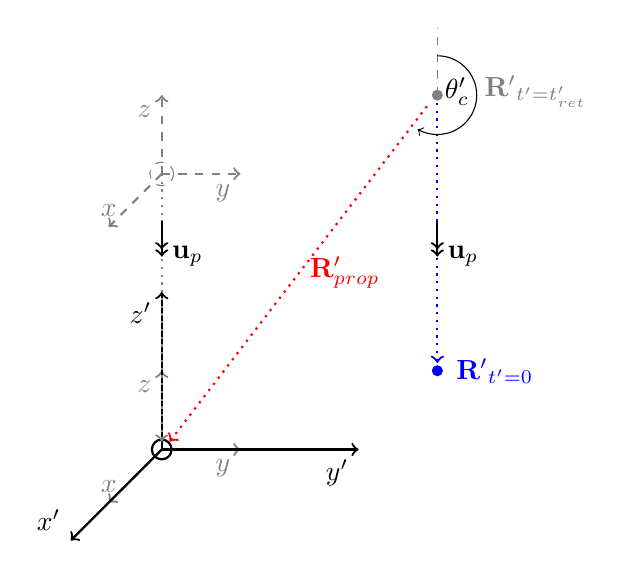
\begin{tikzpicture}[scale=5] %[,tdplot_main_coords]
%\usetikzlibrary{arrows.meta}
\draw[thick] (0 ,0) circle (0.025);
\draw[gray,
dashed] (0,0.7,0) circle (0.03);
\draw[blue,thick,dotted,->] (0.7,0.9,0) -- (0.7,0.22,0); %node[midway,left]{\textcolor{black}{  $\mathbf{P}'$}}; %$\mathbf{P}'$}};
\draw[gray,dashed, thick,->] (0,0.7,0) -- (0.2,0.7,0) node[anchor=north east]{$y$};
\draw[gray,dashed, thick,->] (0,0.7,0) -- (0,0.9,0) node[anchor=north east]{$z$};
\draw[gray,dashed, thick,->] (0,0.7,0) -- (0,0.7,0.35) node[anchor=south] {$x$};
\draw[gray,dashed, thick,->] (0,0,0) -- (0.2,0,0) node[anchor=north east]{$y$};
\draw[gray,dashed, thick,->] (0,0,0) -- (0,0.2,0) node[anchor=north east]{$z$};
\draw[gray,dashed, thick,->] (0,0,0) -- (0,0,0.35) node[anchor=south] {$x$};
\draw[thick,->] (0,0,0) -- (0.5,0,0) node[anchor=north east]{$y'$};
\draw[thick,->] (0,0,0) -- (0,0.4,0) node[anchor=north east]{$z'$};
\draw[thick,->] (0,0,0) -- (0,0,0.6) node[anchor=south east] {$x'$}; 
%\draw[gray,->] (0,0.25,0) to[bend left=40] (0.15,0.2,0);
\draw[red, thick, dotted,<-] (0.02,0.02,0) -- (0.68,0.88,0) node[midway, right] {$\mathbf{R}'_{prop}$};
\draw[gray, thick, dotted,->] (0,0.7,0) -- (0,0.02,0);
\fill[gray] (0.7,0.9,0) circle (0.4pt);
\fill[blue] (0.7,0.2,0) circle (0.4pt) node[right] {\text{ $\mathbf{R'}_{t'=0}$}};
\draw[thick,->>] (0,0.58,0) -- (0,0.49,0) node[right]{$\mathbf{u}_p$};
\draw[ thick,->>] (0.7,0.58,0) -- (0.7,0.49,0) node[right]{$\mathbf{u}_p$};
\draw[gray,dashed] (0.7,0.9,0) -- (0.7,1.07,0);
\draw[->] (0.7,1,0) arc (90:-120:0.1);
\node at (0.75,0.91,0) {$\theta'_c$};
\node[gray] at (0.95,0.91,0) {$\mathbf{R'}_{t'=t'_{ret}}$};
\end{tikzpicture}
\caption{\hyperlink{def-Primed-Frame}{primed frame}}
%  \label{fig:sub2}
\end{subfigure}
\caption{ Diagram of source particle (blue) emitting light (red), which is absorbed by an \protect\hyperlink{def-observer}{observer} positioned at the origin at time $t=t'=0$ with the with the \protect\hyperlink{def-observer}{observer} and source at rest in the first inertial frame (left) and then moving in a \protect\hyperlink{def-Primed-Frame}{primed frame} (right).}
\label{fig: Retarded field}
\end{figure}
When looking at moving objects we see them where they were in their past positions, due to the delay in the light signal, so lets talk about the \hyperlink{def-transform}{transform} showing a source particle emitting a photon to an \hyperlink{def-observer}{observer}, showing the \hyperlink{def-retarded-position}{retarded position}  the \hyperlink{def-observer}{observer} sees.
... explain how observing from earth works, as you would think the positions of stars at $t'=0$ would be all over the place as it rotates around sun
... check equations (since I have everything in opposite directions in diagram, need to change equations?)
We know that a light signal will not instantaneously travel from one point to another it will take time as it travels at the speed of light, so this signal will be delayed/retarded.

system:
If we take the \hyperlink{def-proper-frame}{rest frame} of an \hyperlink{def-observer}{observer} and source particle that emits a pulse of light from its position at $\mathbf{R}$ so that it is received by the \hyperlink{def-observer}{observer} at the origin, at time $t=0$. This would give the Propagation time as $T_{prop}= \frac{|\mathbf{R}|}{c}$ (and hence the time the pulse was emitted as $t_{ret}=-T_{prop}$) and the velocity of the lights propagation $\mathbf{c} = -c \frac{\mathbf{R}}{|\mathbf{R}|}$. and the angle $\theta_{\scalebox{0.5}{R}} = \theta_c - \pi$

\begin{equation}%%%%%%%%%%%%%%%
    \mathbf{R} =  c T_{prop} \begin{pmatrix}
    0\\ \sin{\theta_{\scalebox{0.5}{R}}} \\ \cos{\theta_{\scalebox{0.5}{R}}}
    \end{pmatrix}
    =  - c T_{prop} \begin{pmatrix}
    0\\ \sin{\theta_c} \\ \cos{\theta_c}
    \end{pmatrix}
\end{equation}%%%%
and velocity of light given as
\begin{equation}%%%%%%%%%%%%%%%
    \mathbf{c} = c \begin{pmatrix}
    0\\ \sin{\theta_c} \\ \cos{\theta_c}
    \end{pmatrix}
\end{equation}%%%%

The particle emits the pulse at time $t=t_{ret}$ from $\mathbf{R}$, so this corresponds to the primed position 

\begin{equation}%%%%%%%%%%%%%%%
\begin{aligned}
     \mathbf{R}'_{ret} &=  \begin{pmatrix}
    0\\ c t_{prop}\sin{\theta_{\scalebox{0.5}{R}}} \\ \gamma \left( c t_{prop}\cos{\theta_{\scalebox{0.5}{R}}} - vt_{ret} \right)\\
    \end{pmatrix} = ct_{ret}
    \begin{pmatrix}
    0\\ \sin{\theta_c} \\ \gamma \left( \cos{\theta_c} - \frac{v}{c} \right)\\
    \end{pmatrix} \\
    \text{at time }& \\
    t' &= 
    \gamma (t_{ret} - \frac{v}{c^2} (c t_{prop}\cos{\theta_{\scalebox{0.5}{R}}}) = 
     \gamma t_{ret}(1-\frac{v}{c}  \cos{\theta_c} )  
\end{aligned}        
\end{equation}%%%%

we can see that this does agree with the lights velocity \hyperlink{def-transform}{transform} as well, as it is in the direct opposite direction to $\mathbf{R}$ as it should be. With the light being received at the origin of the \hyperlink{def-Primed-Frame}{primed frame} axis at time $t'=0$

%███████████████████████████████████████████████████████████████████
%███████████████████████████████████████████████████████████████████
\section{Variables}

$R_{prop}, t_{prop}$ \newline

$t_{ret}$ \newline

$R_{ret}$ \newline

\AA  \newline

$\Phi_r$ \newline

$\Phi_{\Omega}$ \newline

$\theta_c$ \newline

$\theta_R$ \newline

$R'_{t'=0}$ \newline

$T_{prop}$ \newline



%███████████████████████████████████████████████████████████████████
%███████████████████████████████████████████████████████████████████
%███████████████████████████████████████████████████████████████████
\chapter{Invariant Quantities TODO}
\hyperlink{def-lorentz-invariant}{lorentz invariance} of different 4 vectors, i.e. 4 position, 4 velocity, and 4 energy momentum vector
... If a physical quantity is \hyperlink{def-lorentz-invariant}{lorentz invariant} it means it is unchanged by a \hyperlink{def-lorentz-transform}{Lorentz transformation} 
... having conserved quantities helps us model complex systems and experiments (frame independent quantity)


Most of this is not as straight forward as previous chapters, and more hard to relate to previous coordinates, velocity and acceleration transforms as energy is a more abstract concept, but the main reason we cared about energy in classical physics is because it was a conserved quantity which is extremely important in classical mechanics, as it gives us tools to make calculations.

... we will try and find a quantity with the units of energy that will have a conservation principle associated
... the derivations to get the famous $E=mc^2$ use approximations, and assumptions and redefined definitions of energy and momentum, and the energy-momentum relation used quantum mechanics to derive, which would require another handbook to go into
... so instead we use the most important thing we need for energy to be and that is to have a associated conservation rule, which means finding an quantity that is unchanged between frames and has a quantity with the units of energy
... to do this we will start from the "4 vector" "4 position" which we already know the associated conservation rule from
... The \hyperlink{def-lorentz-invariant}{lorentz invariant} quantities are sometimes called proper time, proper position, proper acceleration.

4-vector will introduce confusion 

%███████████████████████████████████████████████████████████████████
%███████████████████████████████████████████████████████████████████
\section{recap the conserved quantity from space and time coordinates}

We defined the space-time interval between two \hyperlink{def-event}{event}s:

\begin{equation}
    \Delta S^2 = -(c\Delta t)^2 +\Delta x^2 +\Delta y^2 +\Delta z^2
\end{equation}
(can be defined as negative of this) (show this is \hyperlink{def-lorentz-invariant}{invariant} for any primed coordinates)
all inertial frames of reference agree on this interval (can show it always goes to proper coordinates in this form when subbed in)
the proper time between two \hyperlink{def-event}{event}s $\Delta\tau$ is also agreed upon in all inertial frames
and will also therefore agree on derivatives with respect to $\tau$ (where it is the time between two \hyperlink{def-event}{event}s in the same location?), because they will be \hyperlink{def-lorentz-invariant}{invariant}
we have the position of an \hyperlink{def-event}{event} in space-time given as a 4-position vector (what is a 4-vector)
\begin{equation}
     \mathbf{S} = \begin{pmatrix}
         ct\\x\\y\\z
     \end{pmatrix}
\end{equation}

taking a derivative with respect to $\tau$ gives us the 4-velocity 4-vector with $\frac{d}{d\tau} = \frac{dt}{d\tau}\frac{d}{dt} = \gamma_u \frac{d}{dt} $

\begin{equation}
     \mathbf{U} = \frac{d\mathbf{S}}{d\tau} = \gamma_u \frac{d}{dt} \begin{pmatrix}
         ct\\x\\y\\z
     \end{pmatrix} = \gamma_u \begin{pmatrix}
         c \\ u_x \\ u_y \\ u_z
     \end{pmatrix}
\end{equation}
know to show that the magnitude of this is \hyperlink{def-lorentz-invariant}{invariant} by showing all primed velocities give
\begin{equation}
     ||\mathbf{U}|| = c
\end{equation}

The 4 momentum is defined as
\begin{equation}
    \mathbf{P} = m_0 \mathbf{U} =  \begin{pmatrix}
         \gamma_u m_0 c \\ \gamma_u m_0 u_x \\ \gamma_u m_0 u_y \\ \gamma_u m_0 u_z
     \end{pmatrix}
\end{equation}



we have the Taylor series expansion of $\gamma_u$ factor is
\begin{equation}
    \gamma_u = 1 + \frac{1}{2}\frac{u^2}{c^2} + \frac{3}{8}\frac{u^4}{c^4} + ...
\end{equation}
when subbed into 4-momentum, we have the time component and multiply by $c$, we have 
\begin{equation}
   c \mathbf{P}_t = m_0 c^2\gamma_u = m_0 c^2 ( 1 + \frac{1}{2}\frac{u^2}{c^2} +\frac{3}{8}\frac{u^4}{c^4} + ... ) 
\end{equation}
\begin{equation}
   c \mathbf{P}_t = m_0 c^2  + \frac{1}{2} m_0 u^2  + \frac{3}{8}\frac{u^4}{c^2} + ... ) 
\end{equation}
all terms here are in units of energy, the second term is the classical kinetic energy, and the higher-order terms may be seen as higher order kinetic energy terms that are very small for $u<<c$, the first term does not rely on the velocity of a mass, but only the mass itself, and this can be taken as a new type of energy all masses have even when at rest, i.e. the energy at rest for a mass is
\begin{equation}
    E_{rest} = m_0 c^2 
\end{equation}
we will write this new energy into the 4-momentum
\begin{equation}
    \mathbf{P} = \begin{pmatrix}
         \frac{E}{c} \\ \gamma_u m_0 u_x \\ \gamma_u m_0 u_y \\ \gamma_u m_0 u_z
     \end{pmatrix}
\end{equation}
the magnitude of the 4-momentum can easily be found to be
\begin{equation}
    ||\mathbf{P}|| = m_0 c
\end{equation}
another conserved quantity that does not depend on the frame and using this and the 4-momentum vector
\begin{equation}
    m^2_0 c^2 = - \frac{E^2}{c^2}  + (\gamma_u p_x)^2 + (\gamma_u p_y)^2 + (\gamma_u p_z)^2 = - \frac{E^2}{c^2}  + (\gamma_u p)^2
\end{equation}
giving
\begin{equation}
    E^2 = m_0^2c^4 +\gamma^2p^2c^2
\end{equation}
for stationary particles $u=0$
\begin{equation}
    E = m_0c^2 
\end{equation}
this does not work for a massless particles like photons, we have to use a different method of getting this, we know from before that $ \mathbf{P}^2 = m_0^2 c^2 = 0$ leading to the components giving
\begin{equation}
    \frac{E^2}{c^2} = |p_{light}|^2
\end{equation}
and finally
\begin{equation}
    E = c p_{light}
\end{equation}

....
not needed:
definition of momentum for light borrowed from quantum mechanics
\begin{equation}
    p = \frac{hf}{c}
\end{equation}
where $h$ is Planks constant and $f$ is the frequency of the light
so that the
....

the reason we use this abstract 4-momentum, is because it is conserved and the Newtonian momentum is not conserved when it comes to special relativity


%███████████████████████████████████████████████████████████████████
\subsection{4-Acceleration}
... this is more complex and one difference in this 4-vector here is that the spacial part of the 4-acceleration is not parallel to the 3-acceleration in a \hyperlink{def-Primed-Frame}{primed frame} 
\begin{equation}
    \mathbf{A} = \gamma_u^4 \begin{pmatrix}
         -c\frac{\mathbf{a}\cdot\mathbf{u}}{c^2} \\ \frac{1}{\gamma_u^2} a_x - u_x \frac{\mathbf{a}\cdot\mathbf{u}}{c^2}\\ \frac{1}{\gamma_u^2} a_y - u_y \frac{\mathbf{a}\cdot\mathbf{u}}{c^2} \\ \frac{1}{\gamma_u^2} a_z - u_z \frac{\mathbf{a}\cdot\mathbf{u}}{c^2}
     \end{pmatrix}
\end{equation}

this is not really the same thing as what we think of when we think of acceleration, as it does not give the rate of change of velocity in the normal sense in 3d space

\begin{equation}
    A=\dfrac{dV}{d\tau}=\dfrac{dt}{d\tau}\cdot\dfrac{dV}{dt} \;\;\leftrightarrow\;\; \dfrac{dt}{d\tau}\cdot \dfrac{d}{dt}\left(\begin{array}{*{20}{c}} \gamma_u c \\ \gamma_u u \\ 0 \\ 0 \end{array}\right) = \gamma_u\left(\begin{array}{*{20}{c}} \dfrac{u}{c}\;\gamma_u^3\;a \\ \dfrac{u^2}{c^2}\;\gamma_u^3\;a+\gamma_u a \\ 0 \\ 0 \end{array}\right) = \left(\begin{array}{*{20}{c}} \dfrac{u}{c}\;\gamma_u^4\;a \\ \gamma_u^2\left(\dfrac{u^2}{c^2}\;\gamma_u^2+1\right)a \\ 0 \\ 0 \end{array}\right) = \gamma_u^4\;a\left(\begin{array}{*{20}{c}} \dfrac{u}{c} \\ 1 \\ 0 \\ 0 \end{array}\right)
\end{equation}

%███████████████████████████████████████████████████████████████████
\subsection{4-force}
\begin{equation}
    \mathbf{F}= \frac{d\mathbf{p}}{d\tau} = m_0\mathbf{A}
\end{equation}

%███████████████████████████████████████████████████████████████████
%███████████████████████████████████████████████████████████████████
\section{Energy-Mass Equivalence}

*** E=mc2 is derived using an approximation for v<<c

Imagine we have a particle at rest emitting light in all directions so that afterwards it is still at rest, but in another frame we have we have this particle moving and the emitted light aberrated, but we still need the particle to remain at a constant velocity after emission. (maybe include a rotation in the impulse/effect of light in each direction on particle of has)


- if we have a ball in its \hyperlink{def-proper-frame}{rest frame} that emits a flash of light evenly in all directions, we will have the balls energy decrease by the amount of energy of the emitted light, and it will remain at rest after due to the light being emitted evenly in all directions
- its kinetic energy is zero in this frame

%███████████████████████████████████████████████████████████████████
%███████████████████████████████████████████████████████████████████
\section{Energy-Momentum (Equivalence)}

*** Dirac derived this and used quantum mechanics to do so, which is out of this handbooks domain, still consequences of this equation to be explored, such as the "zitterbewegung"

Momentum in special relativity is defined slightly differently, to ensures that the law of conservation of momentum holds true in all inertial frames, as required by the first postulate of relativity (it is still approximately unchanged at low velocities). momentum of a particle with rest mass $m_0$ is given the 
\begin{equation}%%%%%%%%%%%%%%%
    \mathbf{p'} = m_0 \frac{dR'}{d\tau}= \gamma_u' m_0 \frac{dR'}{dt'} = \gamma m_0 u'
\end{equation}%%%%
where $u'$ is the velocity of the particle in this \hyperlink{def-Primed-Frame}{primed frame} and $\gamma_{u'}= 1/\sqrt{1-u'^2/c^2}$. you will some times the mass of an object referred to as $m=\gamma_{u'} m_0$ which is the apparent mass of a moving particle.

(why not use 3d time differential equation here?)

%███████████████████████████████████████████████████████████████████
%███████████████████████████████████████████████████████████████████
\section{Force Transform TODO}

*** one of the most confusing topics in special relativity, from the way it is defined, how its derived, and how it relates to other things\newline

*** (a note that the 3-force in special relativity is specifically defined as the time derivative of momentum $\frac{d\mathbf{p}}{dt}$ and not not mass times the acceleration $m\mathbf{a}$, this is due to newtons 2nd law holding only for the first definition in special relativity) \newline
*** This means that acceleration turns out not to be in the same direction as the force in special relativity\newline

force derivation is confusing as most sources give the time derivative of u and v as acceleration, (are they using each force has opposite and equal force, but that would not take into account the retardedness)

\begin{equation}%%%%%%%%%%%%%%%
    \mathbf{a} = \frac{1}{m_0 \gamma(\mathbf{v})} \left( \mathbf{F} - \frac{ ( \mathbf{v} \cdot \mathbf{F} ) \mathbf{v} }{c^2} \right)
\end{equation}%%%%

\begin{equation}%%%%%%%%%%%%%%%
    \mathbf{F} = \gamma^3 m_0 \, \mathbf{a}_\parallel + \gamma m_0 \, \mathbf{a}_\perp
\end{equation}%%%%

%███████████████████████████████████████████████████████████████████
\subsection{not sure what this is}
The force parallel to the velocity of the \hyperlink{def-Primed-Frame}{primed frame} is unchanged, $\mathbf{F}_{\parallel \langle ' \rangle} =\mathbf{F}_{\parallel}$, and the force perpendicular to this is $\mathbf{F}_{\perp \langle ' \rangle} =\gamma \mathbf{F}_{\perp}$, with total force, $\mathbf{F}=\mathbf{F}_{\parallel}+\mathbf{F}_{\perp}$ and
\begin{equation}%%%%%%%%%%%%%%%
    \mathbf{F}_{\parallel} = \dfrac{(\mathbf{F}\cdot\mathbf{v})}{|\mathbf{v}|^2}\mathbf{v}
\end{equation}%%%%
and substituting this into formula for total force:
\begin{equation}%%%%%%%%%%%%%%%
    \mathbf{F}_{\perp} = \mathbf{F}-\dfrac{(\mathbf{F}\cdot\mathbf{v})}{|\mathbf{v}|^2}\mathbf{v}
\end{equation}%%%%
since $\mathbf{F}_{\langle ' \rangle} =\mathbf{F}_{\parallel \langle ' \rangle} +\mathbf{F}_{\perp\langle ' \rangle}$ we can use equations above to get:
\begin{equation}%%%%%%%%%%%%%%%
    \begin{split}
    \mathbf{F}_{\langle ' \rangle}  &= \dfrac{(\mathbf{F}\cdot\mathbf{v})}{|\mathbf{v}|^2}\mathbf{v} + \gamma\bigg(\mathbf{F}-\dfrac{(\mathbf{F}\cdot\mathbf{v})}{|\mathbf{v}|^2}\mathbf{v}\bigg)\\
    &= \gamma\mathbf{F} + (1-\gamma)\dfrac{(\mathbf{F}\cdot\mathbf{v})}{|\mathbf{v}|^2}\mathbf{v}
    \end{split}
\end{equation}%%%%
this is the same for electric field as it only differs by a magnitude to the force.\newline
this is similar to how we get the reverse transform: (is it the primed velocity used in this?)
\begin{equation}%%%%%%%%%%%%%%%
    \mathbf{F} = \dfrac{1}{\gamma}\mathbf{F}_{\langle ' \rangle}  + (1-\dfrac{1}{\gamma})\dfrac{(\mathbf{F}_{\langle ' \rangle} \cdot\mathbf{v}_{\langle ' \rangle} )}{|\mathbf{v}_{\langle ' \rangle} |^2}\mathbf{v}_{\langle ' \rangle} 
\end{equation}%%%%

%███████████████████████████████████████████████████████████████████
%███████████████████████████████████████████████████████████████████
\section{Variables}

$\delta S$ \newline

$\vec{S}$ \newline

$\gamma_u$ \newline

$m_0$ \newline

$\vec{P}_t$ \newline

$E_{rest}$ \newline

$E$ \newline

$\vec{P}$ \newline

$p_{light}$ \newline

$p, h, f$ \newline

$\vec{A}$ \newline

$\vec{F}$ \newline

$..._{parralel} ..._{perp}$ \newline

$\vec{F}_{<'>}$ \newline



%███████████████████████████████████████████████████████████████████
\chapter{equation for motion in primed frame for arbitrary proper frame motion}

%███████████████████████████████████████████████████████████████████
\chapter{None Point Like Sources}
... and seeing moving objects rotated, i.e. can see side the rear side of cube before the rear side has moved past you
%███████████████████████████████████████████████████████████████████
\chapter{Thought Experiments}
Bells Paradox and others
%███████████████████████████████████████████████████████████████████
\chapter{Applications}
e=mc2 and kinematics of relativistic classical particles and that....\newline
... touch on GR, i.e. elevator thought experiment
%███████████████████████████████████████████████████████████████████
\chapter{Steps for Frame Swapping}

steps to take when going between frames